% !TeX root = rapport.tex
\documentclass[11pt]{report}
% packages and definitions
\usepackage[utf8]{inputenc}
\usepackage[T1]{fontenc}
\usepackage{graphicx}
\usepackage{amsmath,amssymb}
\usepackage{hyperref}
\usepackage[french]{babel}
\usepackage{url}
% tables
\usepackage[table,xcdraw]{xcolor}
\usepackage{array}
\usepackage{booktabs}
\usepackage{tabularx}
% 
\usepackage{pgfplots}
\usepackage{stmaryrd}
\usepackage{mathtools}
%
\usepackage{algorithm2e}
\DontPrintSemicolon
\LinesNumbered
\SetKwComment{Comment}{ \# }{ }
\RestyleAlgo{ruled}

\usepackage[bottom]{footmisc}
% \usepackage{MnSymbol}


\usepackage{float}
\usepackage{multirow}
\usepackage[top=1.5cm,bottom=1.5cm,margin=1.35cm]{geometry}
\usepackage{tikz}
\usepackage{tikz-cd}

%%%%%%% left bars
%% https://latex.org/forum/viewtopic.php?t=5580
\usepackage{framed}

% Multi column
\usepackage{multicol}

%    BOXES
\usepackage{awesomebox}
% code syntax highlight
% use pdflatex --shell-escape
% latexmk -pdf -time -silent -pvc -bibtex


% https://tex.stackexchange.com/questions/39147/scale-image-to-page-width
\usepackage{changepage}

\usepackage{tablefootnote}


\sffamily
\renewcommand{\familydefault}{\sfdefault}
% \usepackage{helvet}
\usepackage{avant}

\usepackage{dsfont}  % The distribution package name is doublestroke in TeX Live for the LaTeX package dsfont.

% emojis
\usepackage{fontawesome5}
\usepackage{mfirstuc}

\usepackage{minitoc}



\newcommand{\HRule}{\rule{\linewidth}{0.5mm}}
\newcommand{\ra}{ \ \, \faAngleRight \ \ }

% #2980b9
\definecolor{flatuicolors_blue}{HTML}{2980b9}
% #16a085 
\definecolor{flatuicolors_green}{HTML}{16a085}
% #10ac84
% TODO
% #574b90
\definecolor{flatuicolors_purple}{HTML}{574b90}
% ##786fa6
\definecolor{flatuicolors_purple_light}{HTML}{786fa6}
% #2c2c54
\definecolor{flatuicolors_purple_dark}{HTML}{2c2c54}
% #c44569
\definecolor{flatuicolors_rose}{HTML}{c44569}
% #f19066
\definecolor{flatuicolors_orange_light}{HTML}{f19066}
% #e66767
\definecolor{flatuicolors_red_light}{HTML}{e66767}
% #303952
\definecolor{flatuicolors_biscay}{HTML}{303952}
% #546de5
\definecolor{flatuicolors_corn_flower}{HTML}{546de5}
% #222f3e
\definecolor{flatuicolors_imperial}{HTML}{222f3e}
% #01a3a4
\definecolor{flatuicolors_aqua}{HTML}{01a3a4}
% #0abde3
\definecolor{flatuicolors_blue_light}{HTML}{0abde3}
% #54a0ff
\definecolor{flatuicolors_blue_deep}{HTML}{54a0ff}
% #227093
\definecolor{flatuicolors_blue_devil}{HTML}{227093}
% #f368e0
\definecolor{flatuicolors_magenta}{HTML}{f368e0}
% #ff9f43
\definecolor{flatuicolors_orange}{HTML}{ff9f43}
% #ffb142
\definecolor{flatuicolors_yellow}{HTML}{ffb142}
% #eb2f06
\definecolor{flatuicolors_tomato}{HTML}{eb2f06}


%% thm
% \usepackage{theorem}
\usepackage{amsthm}

\newtheoremstyle{def_style}%                % Name
{10pt}%                                     % Space above
{10pt}%                                     % Space below
% {\itshape}%
{}                             % Body font
{0pt}%                                     % Indent amount
{\bfseries}%                            % Theorem head font
{ }%                                    % Punctuation after theorem head
{.5em}%                                    % Space after theorem head, ' ', or \newline
{}% 

\newtheoremstyle{thm_style}%                % Name
{15pt}%                                     % Space above
{15pt}%                                     % Space below
% {\itshape}%                             % Body font
{}
{0pt}%                                     % Indent amount
{\bfseries}%                            % Theorem head font
{ }%                                    % Punctuation after theorem head
{\newline}%                                    % Space after theorem head, ' ', or \newline
{}% 


% \theorembodyfont{\sffamily}
% \theoremheaderfont{\bfseries}

%% ========================================= %%

\theoremstyle{def_style}

\newtheorem{definition}{Définition}
\newtheorem*{definition*}{Définition}

%% ========================================= %%

\theoremstyle{thm_style}

\newtheorem{thm}{Théorème}
\newtheorem{prop}[thm]{Proposition}
\newtheorem{lem}[thm]{Lemme}
\newtheorem*{thm*}{Théorème}
\newtheorem*{propriete*}{Propriété}
\newtheorem*{cor}{Corollaire}

\newtheorem{exo}{Exercice}

\newtheoremstyle{rem_style}%                % Name
{5pt}%                                     % Space above
{5pt}%                                     % Space below
% {\itshape}%
{}                             % Body font
{0pt}%                                     % Indent amount
{\emph}%                            % Theorem head font
{ :}%                                    % Punctuation after theorem head
{.5em}%                                    % Space after theorem head, ' ', or \newline
{}% 

\theoremstyle{rem_style}
\newtheorem*{rem}{Remarque}

%% ========================================= %%


\newcommand{\lorem}{Lorem ipsum dolor sit amet. Ut expedita sunt est delectus quia ad nostrum delectus eum magni dolor. Eos nemo minima sit deleniti porro et necessitatibus minima ab quia necessitatibus in beatae autem et voluptas labore.}

\newcommand{\sssection}[1]{\subsubsection{ \faSquare[regular] #1 }}


\graphicspath{{Images/}} %le chemin vers les images

\pgfplotsset{compat = newest,
	soldot/.style={color=flatuicolors_green,only marks,mark=*},
	holdot/.style={color=flatuicolors_green,fill=white,only marks,mark=*}}

\setlength{\footnotesep}{1.5em}

\renewcommand{\footnoterule}{%
	\kern -3pt
	\hrule width \textwidth height 1pt
	\kern 2pt
}

\usemintedstyle{one-dark}

\renewcommand{\theparagraph}{\thesubsection \quad \small{\faSquare[regular]} \, \Alph{subsubsection}.\alph{paragraph}$\rangle$}
\renewcommand{\thesubsubsection}{\thesubsection \quad \small{\faSquare[regular]} \, \Alph{subsubsection}$\rangle$}
\setcounter{secnumdepth}{4}

\bibliographystyle{plain}

%%%%%%%%%%%%%%%%%%%%%%%%%%%%%%%%%%%%
\newcommand{\auteur}{Hugo Brunet}
\newcommand{\articletitle}{Estimation adaptative en analyse des données fonctionnelles}
\newcommand{\customdate}{Avril—Septembre 2023}
%%%%%%%%%%%%%%%%%%%%%%%%%%%%%%%%%%%%

\dominitoc
\begin{document}
%%%%%%%%%%%%%%%%%%%%%%%%%% INCLUDE COMMAND %%%%%%%%%%%%%%%%%%%%%%%%%%%%%
%%%%%%%%%%%%%%%%%%%%%% AND DEFAULTS PARAMETERS %%%%%%%%%%%%%%%%%%%%%%%%%
%% ================= commandes ========================== 


%%  box
\newcommand{\info}[1]{%
    \awesomebox[flatuicolors_blue]{2pt}{\faInfoCircle}{flatuicolors_blue}{#1}%
}

\newcommand{\chk}[1]{%
\awesomebox[flatuicolors_green]{2pt}{\faCheckCircle}{flatuicolors_green}{#1}%
}

\newcommand{\brain}[1]{%
\awesomebox[flatuicolors_purple_light]{2pt}{[\faBrain ]}{flatuicolors_purple_light}{#1}%
}

\newcommand{\warn}[1]{%
\awesomebox[flatuicolors_orange_light]{2pt}{\faExclamationTriangle}{flatuicolors_orange_light}{#1}%
}

\newcommand{\nope}[1]{%
\awesomebox[flatuicolors_red_light]{2pt}{\faTimesCircle}{flatuicolors_red_light}{#1}%
}

\newcommand{\cogs}[1]{%
\awesomebox[flatuicolors_imperial]{2pt}{\faCogs}{flatuicolors_imperial}{#1}%
}

\newcommand{\citer}[1]{%
\awesomebox[flatuicolors_corn_flower]{2pt}{\faQuoteRight}{flatuicolors_corn_flower}{#1}%
}


\newcommand{\avion}[1]{%
    \awesomebox[flatuicolors_purple_dark]{2pt}{\faFighterJet}{flatuicolors_purple_dark}{#1}%
}


\newcommand{\flask}[1]{%
    \awesomebox[flatuicolors_blue_devil]{2pt}{\faFlask}{flatuicolors_blue_devil}{#1}%
}


\newcommand{\idee}[1]{%
    \awesomebox[flatuicolors_yellow]{2pt}{\faLightbulb}{flatuicolors_yellow}{#1}%
}


\newcommand{\book}[1]{%
    \awesomebox[flatuicolors_orange_light]{2pt}{\faBook}{flatuicolors_orange_light}{#1}%
}

\newcommand{\question}[1]{%
    \awesomebox[flatuicolors_aqua]{2pt}{\faQuestion}{flatuicolors_aqua}{#1}%
}

% \usetikzlibrary{shapes, backgrounds}
\tikzset{x=1cm, y=1cm} % Default tikz units

% Command to vertically centre adjacent content
\newcommand{\vcenteredhbox}[1]{% The only parameter is for the content to centre
	\begingroup%
		\setbox0=\hbox{#1}\parbox{\wd0}{\box0}%
	\endgroup%
}


\newcommand{\cvsect}[1]{% The only parameter is the section text
	\vspace{\baselineskip} % Whitespace before the section title
	\colorbox{black}{\textcolor{white}{\MakeUppercase{\textbf{#1}}}}\\% Section title
}
\newcommand{\blackboxed}[1]{%
\colorbox{black}{\textcolor{white}{\textbf{#1}}}%
}

\newcommand{\icon}[3]{% The first parameter is the FontAwesome icon name, the second is the box size and the third is the text
	\vcenteredhbox{\colorbox{black}{\makebox(#2, #2){\textcolor{white}{\large\csname fa#1\endcsname}}}}% Icon and box
	\hspace{0.2cm}% Whitespace
	\vcenteredhbox{\textcolor{black}{#3}}% Text
}


%%%%%%%% VARIANTES COLOREES	%%%%%%%%%%%%


\newcommand{\redboxed}[1]{%
\colorbox{flatuicolors_tomato}{\textcolor{white}{\textbf{#1}}}%
}

\newcommand{\greenboxed}[1]{%
\colorbox{flatuicolors_green}{\textcolor{white}{\textbf{#1}}}%
}

\newcommand{\blueboxed}[1]{%
\colorbox{flatuicolors_blue_devil}{\textcolor{white}{\textbf{#1}}}%
}

\newcommand{\purpleboxed}[1]{%
\colorbox{flatuicolors_purple_dark}{\textcolor{white}{\textbf{#1}}}%
}

\newcommand{\orangeboxed}[1]{%
\colorbox{flatuicolors_orange}{\textcolor{white}{\textbf{#1}}}%
}

\newcommand{\aquaboxed}[1]{%
\colorbox{flatuicolors_aqua}{\textcolor{white}{\textbf{#1}}}%
}


\newcommand*{\circled}[1]{\tikz[baseline=(char.base)]{%
\node[shape=circle,draw,inner sep=2pt] (char) {#1};}%
}
\newcommand{\colorize}[2][flatuicolors_blue]{\color{#1} #2 \color{black}}
\newcommand{\emphcolor}[2][flatuicolors_blue]{%
    \color{#1} \mathbf{#2} \color{black}%
}



\newcommand{\includeimage}[4][0.5]{%
\begin{figure}[h]%
    \centering%
    \includegraphics[width= #1 \textwidth]{#2}%
    \caption{#3}%
    \label{fig: #4 }%
\end{figure}%
} % WIDTH | PATH | CAPTION | label

\newcommand{\el}{\triangleright \quad}
\newcommand{\largeskip}{\bigskip\bigskip\bigskip}
\newcommand{\penguin}{\faQq}


%%  notation convergence
% uses mathtools package
\newcommand{\cvl}[2]{\wrightarrow[#1 \rightarrow #2]{\ \mathcal L \ } \ }
\newcommand{\cvp}[2]{\xrightarrow[#1 \rightarrow #2]{\ \mathbb P \ } }
\newcommand{\cvps}[2]{\xrightarrow[#1 \rightarrow #2]{\ \textsf{p.s}\ } \ }
\newcommand{\cvL}[3]{\xrightarrow[#2 \rightarrow #3]{\ \mathbb L ^{#1} \ }}
\newcommand{\cvetr}[2]{\xrightarrow[#1 \rightarrow #2]{ \ \textsf{étroit.} \ }}
\newcommand{\cvnorme}[3]{\xrightarrow[\, #2 \rightarrow #3 \; ]{\, \lVert \cdot \rVert _{#1} \,} \ }
\newcommand{\cvpp}[3]{ \xrightarrow[#2 \rightarrow #3]{#1 - p.p} }
%%  autres
\newcommand{\tend}[2]{\xrightarrow[ #1 \rightarrow #2 ]{}}
\newcommand{\tendset}[3]{\xrightarrow[ #1 \rightarrow #2 ]{#3}}

\newcommand{\intervaleint}[2]{\llbracket #1 \, , \, #2 \rrbracket}
\newcommand{\R}[1]{\mathds{R} ^{#1}}


\newcommand{\classespace}[2]{\mathcal C^{#1} \left( \, #2 \, \right)}
\newcommand{\continuborne}[2]{\mathcal C^0_b \left( \, #1 \,, \, #2 \, \right)}
\newcommand{\continusupportcompact}[2]{\mathcal C^0_K \left( \, #1 \,, \, #2 \, \right)}
\newcommand{\mesurable}[2]{\mathcal m\left( \, #1 \,, \, #2 \, \right)}
\newcommand{\etageepositive}[2]{\mathcal E_+\left( \, #1 \,, \, #2 \, \right)}
\newcommand{\VA}[1]{\mathds VA \left( \, #1 \, \right)}


\newcommand{\matrixspace}[2]{\mathcal M_{#1} \left( \, #2 \,  \right)}%

\newcommand{\orthonormal}{\underset{\Vert \cdot \Vert}{\perp}}


\newcommand{\grandR}{\mathds R}%
\newcommand{\grandZ}{\mathds Z}%
\newcommand{\grandQ}{\mathds Q}%
\newcommand{\grandN}{\mathds N}%
\newcommand{\grandH}{\mathds H}%
\newcommand{\grandW}{\mathds W}%
\newcommand{\grandT}{\mathds T}%
\newcommand{\grandJ}{\mathds J}%
\newcommand{\grandL}{\mathds L}%
\newcommand{\grandP}{\mathds P}%
\newcommand{\grandK}{\mathds K}%
\newcommand{\grandX}{\mathds X}%
\newcommand{\grandY}{\mathds Y}%
\newcommand{\grandB}{\mathds B}%
\newcommand{\grandM}{\mathds M}%
\newcommand{\grandA}{\mathds A}%
\newcommand{\grandF}{\mathds F}%
\newcommand{\grandI}{\mathds I}%
\newcommand{\grandD}{\mathds D}%
\newcommand{\grandV}{\mathds V}%
\newcommand{\grandE}{\mathds E}%



\newcommand{\calF}{\mathcal F}
\newcommand{\calO}{\mathcal O}
\newcommand{\calL}{\mathcal L}
\newcommand{\calP}{\mathds P}
\newcommand{\calM}{\mathds M}



\newcommand{\Rplus}{\mathds R_+}
\newcommand{\Rmoins}{\mathds R_-}


\newcommand{\indicatrice}[1]{\mathds 1 _{#1}}
\newcommand{\norme}[2]{\lVert \, #2 \, \rVert _ {#1}}
\newcommand{\dist}[2]{ \ \lVert #1 - #2 \rVert \ }
\newcommand{\distnorme}[3]{ \norme{#1}{#2 - #3}}

\newcommand{\prodscal}[2]{\left\langle \, #1 \, \vert \, #2 \, \right\rangle}
\newcommand{\prodscalselon}[3]{\prodscal{#1}{#2}_{#3}}

% \argmax\limits_{}
\newcommand{\argmax}{\operatornamewithlimits{argmax}}
\newcommand{\argmin}{\operatornamewithlimits{argmin}}

\newcommand{\inverse}[1]{#1 ^ {-1}}

\newcommand{\isdef}{\underset {\textsf{déf}} {\equiv}}
\newcommand{\comm}[1]{\operatorname{Comm}\left( #1 \right)}
\newcommand{\rg}[1]{\operatorname{rg}\left( #1 \right)}
\newcommand{\im}{\operatorname{Im}}
\newcommand{\pgcd}[2]{\operatorname{pgcd}\left( \, #1 , \, #2 \, \right)}

\newcommand{\positive}[1]{\left[ \, #1 \, \right]_+}

\newcommand{\func}[4]{%
	\begin{array}{ccc} #1 &\longrightarrow& #2 \\ #3 &\longmapsto& #4 \end{array}
}%
%%  Landau
\newcommand{\petitop}[1]{\underset \P {\mathcal o} \left( \ #1 \ \right)}
\newcommand{\grandop}[1]{\underset \P {\mathcal O} \left( \ #1 \ \right)}

\newcommand{\preuve}[1]{%
	\begin{leftbar}%
		\begin{proof}%
			\textsf{}%
			\bigskip%
			#1%
		\end{proof}%
	\end{leftbar}%
}


\newcommand{\subproofsmall}[2]{%
	\begin{minipage}{0.005\linewidth}%
		\textsf{ }%
	\end{minipage}%
	\begin{minipage}{0.895\linewidth}%
		\begin{leftbar}%
			\begin{proof}%
				[\faAngleRight \, \fbox{#1}]%
				\textsf{ }%
				\bigskip%
				\\%
				#2%
			\end{proof}%
		\end{leftbar}%
	\end{minipage}%
}

\newcommand{\subproofmedium}[2]{%
	\begin{minipage}{0.1\linewidth}%
		\textsf{ }%
	\end{minipage}%
	\begin{minipage}{0.8\linewidth}%
		\begin{leftbar}%
			\begin{proof}%
				[#1]%
				\textsf{ }%
				\bigskip%
				#2%
			\end{proof}%
		\end{leftbar}%
	\end{minipage}%
}

\newcommand{\subproofbig}[2]{%
	\begin{minipage}{0.2\linewidth}%
		\textsf{ }%
	\end{minipage}%
	\begin{minipage}{0.7\linewidth}%
		\begin{leftbar}%
			\begin{proof}%
				[#1]%
				\textsf{ }%
				\bigskip%
				#2%
			\end{proof}%
		\end{leftbar}%
	\end{minipage}%
}

%% Lettres
\renewcommand{\P}{\mathds P}
\newcommand{\E}{\mathds E}
\newcommand{\V}{\mathds V}
\newcommand{\Q}{\mathds Q}
\newcommand{\IR}{\mathds R}
\newcommand{\IH}{\mathds H}


\newcommand{\indep}{\perp \!\!\! \perp}

\newcommand{\samelaw}{\overset{\mathcal L}{\, \sim \,}}

%   fonctions mathématiques de proba

\newcommand{\proba}[1]{\mathds P \left[ \, #1 \, \right]}
\newcommand{\probaloi}[2]{\mathds P_{#1} \left[ \, #2 \, \right]}
\newcommand{\variance}[1]{\mathds V \left[ \, #1 \, \right]}
\newcommand{\esperance}[1]{\mathds E \left[ \, #1 \, \right]}
\newcommand{\esperanceloi}[2]{\mathds E_{#1} \left[ \, #2 \, \right]}
\newcommand{\esperancesachant}[2]{\mathds E \left[ \, #2 \, \vert \, #1 \, \right]}
\newcommand{\esploisach}[3]{\mathds E \left[ \, #3 \, \vert \, #2 \, \right]_{#1}}
%%  VA spéciales
\newcommand{\statrang}[3]{{#1} _ {#2} ^{\left(#3\right)}}
%%  suites
\newcommand{\suiteensemble}[1]{\left(  #1  \right)^\mathbb N}
\newcommand{\suite}[2]{( {#1}_{#2})_{#2 \geq 0}}
\newcommand{\soussuite}[2]{( {#1}_{n_{#2}})_{#2 \geq 0}}
\newcommand{\famille}[2]{( {#1}_{#2})_{#2 \in I}}
\newcommand{\suitecomposition}[3]{\left( #1( {#2}_{#3}) \right)_{#3 \geq 0}}
\newcommand{\suitestatrang}[3]{ \left( \statrang{#1}{#3}{i} \right)_{#2, #3}}

\newcommand{\famfinie}[4][i]{\left( \, {#2} _ {#1} \, \right)_{#3, #4}}

\newcommand{\fromto}[3]{{#1}_{#2\, ; \, #3}}


\newcommand{\mail}{\href{mailto:allemandinstable@gmail.com}{allemandinstable@gmail.com}}
\newcommand{\github}{\href{https://github.com/allemand-instable/}{allemand-instable}}

\setproofrender{0}
%%%%%%%%%%%%%%%%%%%%%%%%% DEBUT COURVERTURE %%%%%%%%%%%%%%%%%%%%%%%%%%%%%%
\begin{titlepage}

	\begin{center}

		% 	LOGO	/////////////////////////////////////////////
		\textsc{{\LARGE Ecole nationale de la statistique \\et de l'analyse de l'information}} \\ %Nom de l'école
\vspace{5mm}
\begin{minipage}{0.49\textwidth}
    \centering
    
\includegraphics[width=0.95\textwidth]{Images/ensai_logo.png}\\[1.0 cm] %logo de l'école
\end{minipage}
\begin{minipage}{0.49\textwidth}
    \centering
    
\includegraphics[width=0.95\textwidth]{Images/datastom_logo.png}\\[1.0 cm] %logo de l'école
\end{minipage}



		% 	Title	////////////////////////////////////////////
		\textsc{\LARGE Stage de Fin d'Étude }\\[0.5cm]
		{\Large pour l'entreprise DataStorm}\\ [1cm]

		\HRule%
		\vspace{0.4cm}

		{\huge \bfseries \articletitle}\\[0.4cm]
		
		\HRule%
		\vspace{1.5cm}

		version corrigée et augmentée

	\vfill
	\end{center}
	
	
	% ==================== AUTEURS ==================== %
	
	\begin{flushright} \Large
		\textbf{rédigé par}%
		\\
		\auteur%
		\\
		\textbf{Tuteur}%
		\\
		Hassan Maissoro
	\end{flushright}

	% ==================== DATE ============================== %


	\begin{center}
		{\large{\customdate}}
	\end{center}
\end{titlepage}

%%%%%%%%%%%%%%%%%%%%%%%%% FIN COURVERTURE %%%%%%%%%%%%%%%%%%%%%%%%%%%%%%
% \addtocontents{toc}{\protect\thispagestyle{empty}}
\pagenumbering{Roman}
%%%%%%%%%%%%%%%%%%%%%%%%% DEBUT ABSTRACT %%%%%%%%%%%%%%%%%%%%%%%%%%%%%%%%
\begin{abstract}
    \begin{center}
        \fbox{

            \begin{minipage}{0.75\textwidth}
                \lorem%
                
                \lorem%
            \end{minipage}

        }
    \end{center}

    
    \textbf{contribution}

    \bigskip

    si jamais vous apercevez des fautes dans le polycopié, merci de rédiger une \emph{issue} sur Github à l'adresse:

    \bigskip

    \textbf{correctif}

    \awesomebox[flatuicolors_imperial]{2pt}{\faGithub}{flatuicolors_imperial}{\centering{\href{https://github.com/allemand-instable/LaTeX-Template/issues}{LaTeX-Template/issues}}}

    \textbf{contact}
    \awesomebox[flatuicolors_orange_light]{2pt}{\faAt}{flatuicolors_orange_light}{ \center{\textbf{mail DEV:} \href{mailto:dev.allemandinstable@gmail.com}{dev.allemandinstable@gmail.com} }}


\end{abstract}
\pagebreak
%%%%%%%%%%%%%%%%%%%%%%%%% FIN ABSTRACT %%%%%%%%%%%%%%%%%%%%%%%%%%%%%%%%%%
%Ici on insère la table des matières (entre astract et les chapitres)
\section*{Notations}
\thispagestyle{empty}

\begin{table}[H]
	\centering
	\begin{tabularx}{\textwidth}{lX}
		\toprule
		\textbf{Notation}                                                & \textbf{Signification}                                                                                                                                                                                                            \\
		\midrule
		\textbf{Abréviations}                                                                                                                                                                                                                                                                                \\
		\midrule
		CDC                                                              & Courbe de Charge                                                                                                                                                                                                                  \\
		FDC                                                              & Facteur de Charge                                                                                                                                                                                                                 \\
		MPV                                                              & Maissoro - Patilea - Vimond                                                                                                                                                                                                       \\
		FDA                                                              & Analyse de Données Fonctionnelles (Functional Data Analysis)                                                                                                                                                                      \\
		FPCA                                                             & Analyse par Composantes Principales Fonctionnelle(Functional Principal Component Analysis)                                                                                                                                        \\
		KL                                                               & Karhunen-Loève                                                                                                                                                                                                                    \\
		\midrule
		\textbf{Analyse}                                                 &                                                                                                                                                                                                                                   \\
		\midrule
		$x_0$                                                            & Une valeur spécifique de $x$                                                                                                                                                                                                      \\
		$V \in \mathcal{V}(x_0)$                                         & Un voisinage de $x_0$                                                                                                                                                                                                             \\
		$\mathcal C^0(E, F)$                                             & Fonction continue de $E$ dans $F$                                                                                                                                                                                                 \\
		$\mathcal{H}_{\mathcal{V}(x_0)}(\alpha_{x_0}, L_{\alpha_{x_0}})$ & Classe de Hölder de paramètre $\alpha_{x_0}, L_{\alpha_{x_0}}$ sur un voisinage de $x_0$                                                                                                                                          \\
		$\operatorname{mfBm}(H, L)$                                      & Ensemble des mouvements browniens multi-fractionnaires de fonction de Hurst $H : t \mapsto H_t$ et constante de Hölder locale $L : t \mapsto L_t$ : ce sont les \og paramètres de Hölder \fg des mouvements browniens considérés. \\
		\midrule
		\textbf{Algèbre}                                                 &                                                                                                                                                                                                                                   \\
		\midrule
		$\operatorname{sp}_{\mathds K}(\varphi)$                         & Valeurs propres d'un opérateur ou endomorphisme linéaire $\varphi$ sur le corps $\mathds K$                                                                                                                                       \\
		$\operatorname{sp}(\varphi)$                                     & Valeurs propres d'un opérateur ou endomorphisme linéaire $\varphi$ sous-entendu sur le corps $\mathds R$                                                                                                                          \\
		$\overrightarrow{sp}_{\orthonormal}(\varphi)$                    & Vecteurs propres d'un opérateur ou endomorphisme linéaire $\varphi$ formant une famille orthogonale                                                                                                                               \\
		$\overrightarrow{sp}_{\orthonormal}^{[1,p]}(\varphi)$            & $p$ premiers vecteurs propres d'un opérateur ou endomorphisme linéaire $\varphi$ formant une famille orthogonale                                                                                                                  \\
		\midrule
		\textbf{Statistique}                                             &                                                                                                                                                                                                                                   \\
		\midrule
		$X$                                                              & La \og vraie \fg distribution                                                                                                                                                                                                     \\
		$\widetilde{X}$                                                  & Quantité intangible/inobservable                                                                                                                                                                                                  \\
		$\widehat{X}$                                                    & Un estimation empirique X                                                                                                                                                                                                         \\
		$\ordered X k$                                                   & Statistique d'ordre de $X$, $k^{eme}$ terme : $\ordered X {k} \leq \ordered X {k+1}$                                                                                                                                              \\
		$\statrang Y n {k}$                                              & Valeur observée au $k^{eme}$ temps (au sens de la relation d'ordre $\leq$ ) sur le support du processus $X_n$ : $\statrang Y n k \isdef X_n( \ordered T k ) + \eta_{n}[k]$                                                        \\
		\midrule
		\textbf{Probabilités}                                            &                                                                                                                                                                                                                                   \\
		\midrule
		$C_X (s,t)$                                                      & Covariance du processus $X$ entre le temps $s$ et le temps $t$                                                                                                                                                                    \\
		$c\left[ \, f \, \right]$                                        & Opérateur de covariance évalué en $f$                                                                                                                                                                                             \\
		$\mathds V \operatorname{A}\left[ \, E \,\right]$                & Variable aléatoire à valeur dans $E$ : $\mathds V \operatorname{A}\left[ \, E \,\right] \isdef \mathbf m\bigl( \left(\Omega, \mathcal F, \mathds P\right) \, , \, \left(E, \mathcal A, \mu\right) \bigr)$                         \\
		\bottomrule
	\end{tabularx}
\end{table}


\begin{table}[H]
	\centering
	\begin{tabularx}{\textwidth}{lX}
		\toprule
		\textbf{Notation}                                                                               & \textbf{Signification}                                                                                                                                                                                                                                                                                                                      \\
		\midrule
		\textbf{Spécifique au stage}                                                                                                                                                                                                                                                                                                                                                                                                                  \\
		\midrule
		$\xi$                                                                                           & Bruit blanc gaussien provenant d'un mouvement Brownien multi-fractionnaire                                                                                                                                                                                                                                                                  \\
		$\eta$                                                                                          & Bruit blanc gaussien provenant de l'erreur de mesure                                                                                                                                                                                                                                                                                        \\
		\midrule
		$M_n$                                                                                           & Nombre de points observés sur la trajectoire de la donnée fonctionnelle $X_n$                                                                                                                                                                                                                                                               \\
		$N$                                                                                             & Nombre de courbes observées                                                                                                                                                                                                                                                                                                                 \\
		\midrule
		$\lambda$                                                                                       & $\esperance{M_n}$ ( $M_n \sim \mathcal P(\lambda)$ )                                                                                                                                                                                                                                                                                        \\
		$\widehat \lambda$                                                                              & Nombre moyen de points observés par courbe : $\widehat \lambda = \frac 1 N \sum\limits_{i=1}^N M_i$																																																										  \\
		\midrule
		\textbf{Temps particuliers ($t \in \mathcal T$)}                                                &                                                                                                                                                                                                                                                                                                                                             \\
		\midrule
		$\mathcal T$                                                                                    & Support du processus $X$, ici $\mathcal T = [0,1]$                                                                                                                                                                                                                                                                                          \\
		$T_n[m]$                                                                                        & $m^{eme}$ temps ( du $m^{eme}$ sampling du phénomène aléatoire ) observé sur la trajectoire de la donnée fonctionnelle $X_n$                                                                                                                                                                                                                \\
		$T_n^{(m)}$                                                                                     & $m^{eme}$ temps (au sens de la relation d'ordre $\leq$ ) observé sur la trajectoire de la donnée fonctionnelle $X_n$                                                                                                                                                                                                                        \\
		$t_0$ ou $t_2$                                                                                  & Point où l'on souhaite estimer la régularité, $t_0$ est plus courant comme notation pour fixer un point mais $t_2$ est utilisé dans l'implémentation pour signaler sa centralité sur $J_\Delta$                                                                                                                                             \\
		$J_\Delta(t_0)$                                                                                 & \og voisinage \fg du point $t_0$ que l'on utilise pour estimer la régularité, implémenté comme l'intervalle $[t_1, t_3]$                                                                                                                                                                                                                    \\
		$t_1(\Delta)$                                                                                   & $t_2 - \Delta/2$ | lorsque $\Delta$ est quelconque, abbrégé en $t_1$                                                                                                                                                                                                                                                                        \\
		$t_3(\Delta)$                                                                                   & $t_2 + \Delta/2$ | lorsque $\Delta$ est quelconque, abbrégé en $t_3$                                                                                                                                                                                                                                                                        \\
		$g_k$                                                                                           & Point de la grille du calcul numérique d'une intégrale, $k \in \intervaleint 1 G$                                                                                                                                                                                                                                                           \\
		\midrule
		$\phi$                                                                                          & Relation auto-régressive intégrale                                                                                                                                                                                                                                                                                                          \\
		$\beta$                                                                                         & Noyau de l'opérateur intégral                                                                                                                                                                                                                                                                                                               \\
		\midrule
		$\theta(u,v)$                                                                                   & $= \esperance{ |X(v) - X(u)|^2 }$                                                                                                                                                                                                                                                                                                           \\
		\toprule
		\textbf{Utilisés dans les algorithmes}                                                   		&                                                                                                                                                                                                                                                                                                                                             \\
		\midrule
		$\mathds T$                                                                                     & Ensemble des points générés dans la simulation du mouvement brownien multi-fractionnaire : points observés (aléatoire), point de la grille d'approximation de l'intégrale de la relation FAR, points utilisés pour l'estimation de la régularité locale                                                                                     \\
		$B$                                                                                             & Nombre de burn-in pour atteindre la stationnarité du FAR                                                                                                                                                                                                                                                                                    \\
		$G$                                                                                             & Nombre de points de la grille du calcul numérique d'une intégrale                                                                                                                                                                                                                                                                           \\
		\midrule
		$\mathcal R^{[\, rel / abs\,]}_{mc} \bigl( \, \Delta, \Theta \,\bigr)$                          & Risque pour une réplication de Monte-Carlo du couple $\Theta$  :   $\mathcal R^{[\, rel\,]}_{mc} \bigl( \, \Delta, \Theta \,\bigr) = \frac{\distnorme 2 {\widehat \Theta}{\widetilde \Theta}}{\norme 2 \Theta}$ et  $\mathcal R^{[\, abs \,]}_{mc} \bigl( \, \Delta, \Theta \,\bigr) = {\distnorme 2 {\widehat \Theta}{\widetilde \Theta}}$ \\
		$\mathcal R^{[\, rel / abs\,]}_{mc \, \colorize{[\, p \, ]}} \bigl( \, \Delta, \Theta \,\bigr)$ & Risque pour la $p^{eme}$ réplication de Monte-Carlo de la simulation																																																																		  \\
		\midrule
		$\mathcal R^{[\, rel / abs\,]} \bigl( \, \Delta, \Theta \,\bigr)$                               & Risque d'estimation du couple d'incréments pour des réplications indépendantes (de Monte-Carlo) : $\mathcal R^{[\, rel / abs\,]} \bigl( \, \Delta, \Theta \, \bigr) = \mathds E_p \bigl[ \, \mathcal R^{[\, rel / abs\,]}_{mc \, \colorize{[\, p \, ]}} \bigl( \, \Delta, \Theta \,\bigr) \, \bigr]$                                        \\
		$\widehat{\mathcal R}^{[\, rel / abs\,]} \bigl( \, \Delta, \Theta \,\bigr)$                     & Estimation du risque d'estimation du couple d'incréments par la moyenne empirique $\frac 1 {mc} \sum\limits_{p=1}^{mc} \, \mathcal R^{[\, rel / abs\,]}_{mc \, \colorize{[\, p \, ]}} \bigl( \, \Delta, \Theta \,\bigr)$                                                                                                                    \\
		\bottomrule
	\end{tabularx}
	% \label{tab:notation-specifique-stage}
\end{table}

\pagebreak
\tableofcontents
% \thispagestyle{empty}
\pagebreak
\listoffigures
\listoftables
% \listofalgorithms
% \thispagestyle{empty}

%%%%%%%%%%%%%%%%%%%%%%%%% DEBUT CHAPITRES %%%%%%%%%%%%%%%%%%%%%%%%%%%%%%
\chapter{Motivations}
\minitoc%


Dans le cadre de ce stage, les données que l'on traite sont des données du secteur de l'énergie, et plus particulièrement des données de production électrique. On dispose ainsi de plusieurs éoliennes identifiées par le tag "id\_[identifiant de l'éolienne]" dont l'énergie produite est mesurée toutes les demies heures, et ce pendant 4 ans (de de 2014 à 2017).
Cette énergie produite est dénommée la courbe de charge (que l'on abbrégera par \textbf{CDC} par la suite). Il est cependant plus utile de s'intéresser au facteur de charge (ou \textbf{FDC}) qui est défini comme

\begin{equation*}
\displaystyle\textsf{Facteur de Charge} = \frac{\textsf{Courbe de Charge}}{\textsf{Puissance Installée}}
\end{equation*}

On en déduit que \textbf{FDC} doit nécessairement être compris entre 0 et 1. C'est entre autre aussi une manière de détecter des anomalies et données atypiques comme la surproduction d'énergie par rapport à ce qui était attendu de la part d'un parc éolien ou encore un défaut de capteur (tension / intensité, ...) qui mesure la courbe de charge. Voici notamment l'exemple de données éoliennes :


\begin{center}
	période : Première semaine de Juin 2015
	
	\scalebox{1}{
		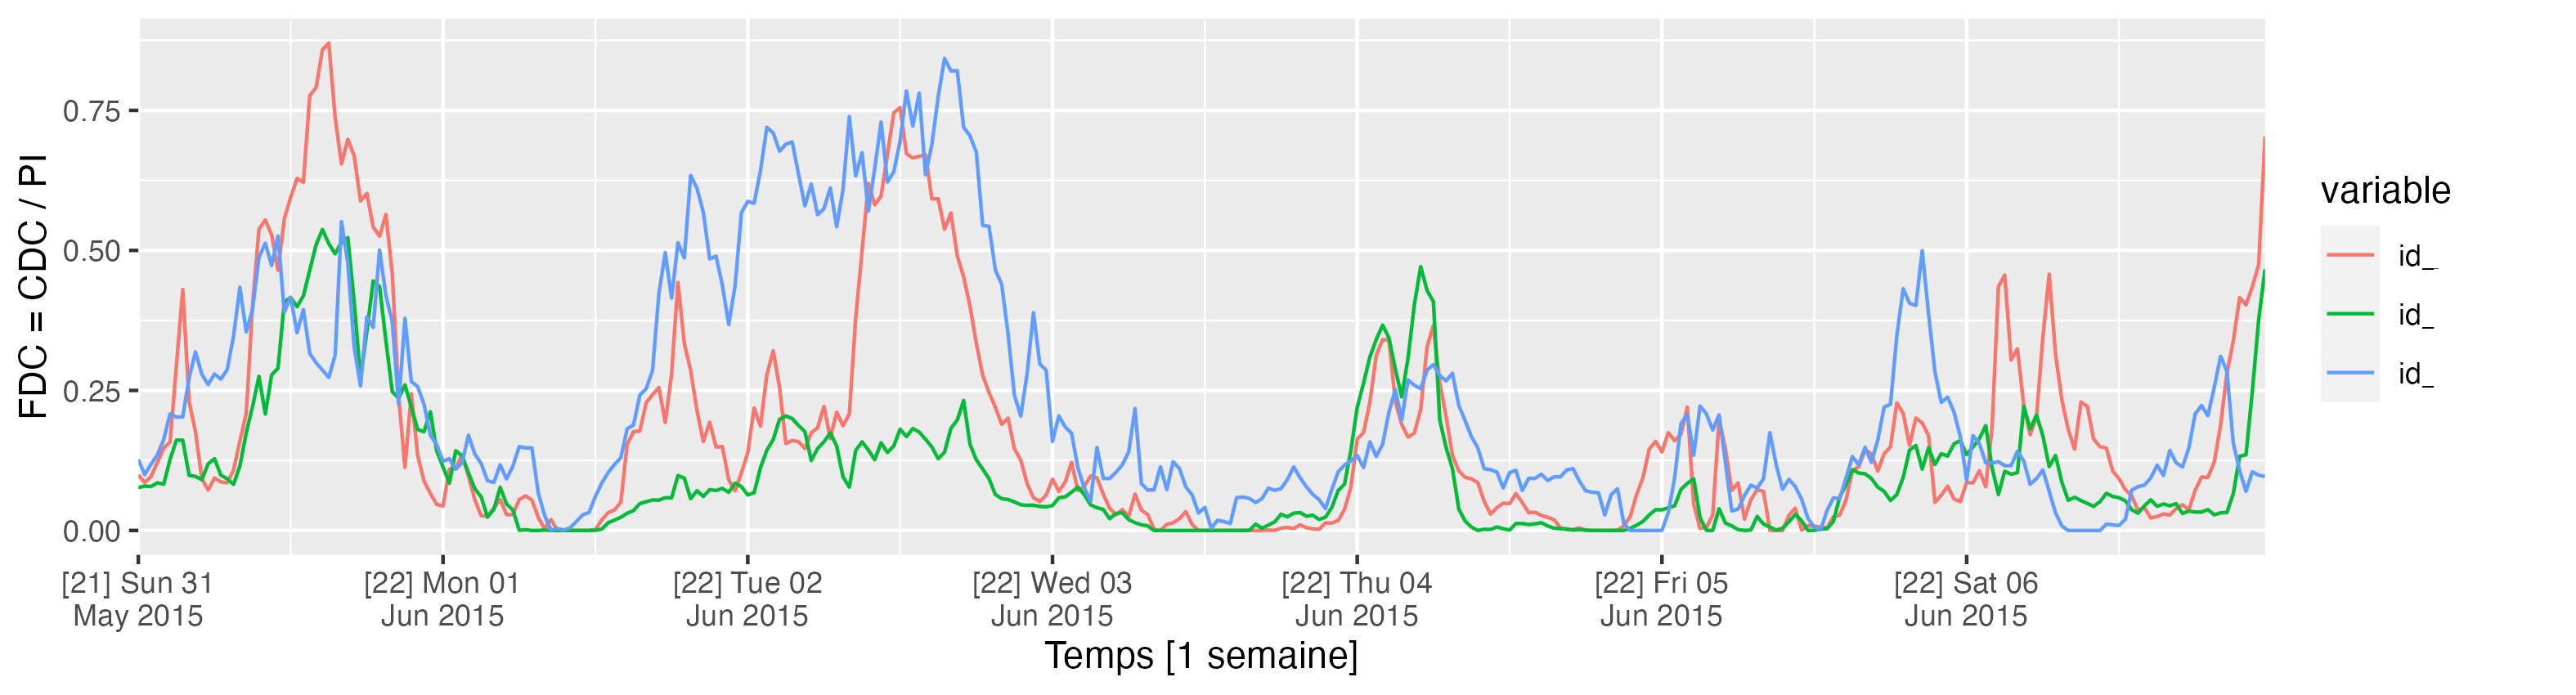
\includegraphics[width=0.85\textwidth]{Images/motivation/test__slice_graph__2015__id_1_2_3__week_1.jpg}
	}
\end{center}

\begin{figure}[H]
	\centering

	période : Juillet 2015

	\scalebox{1}{
		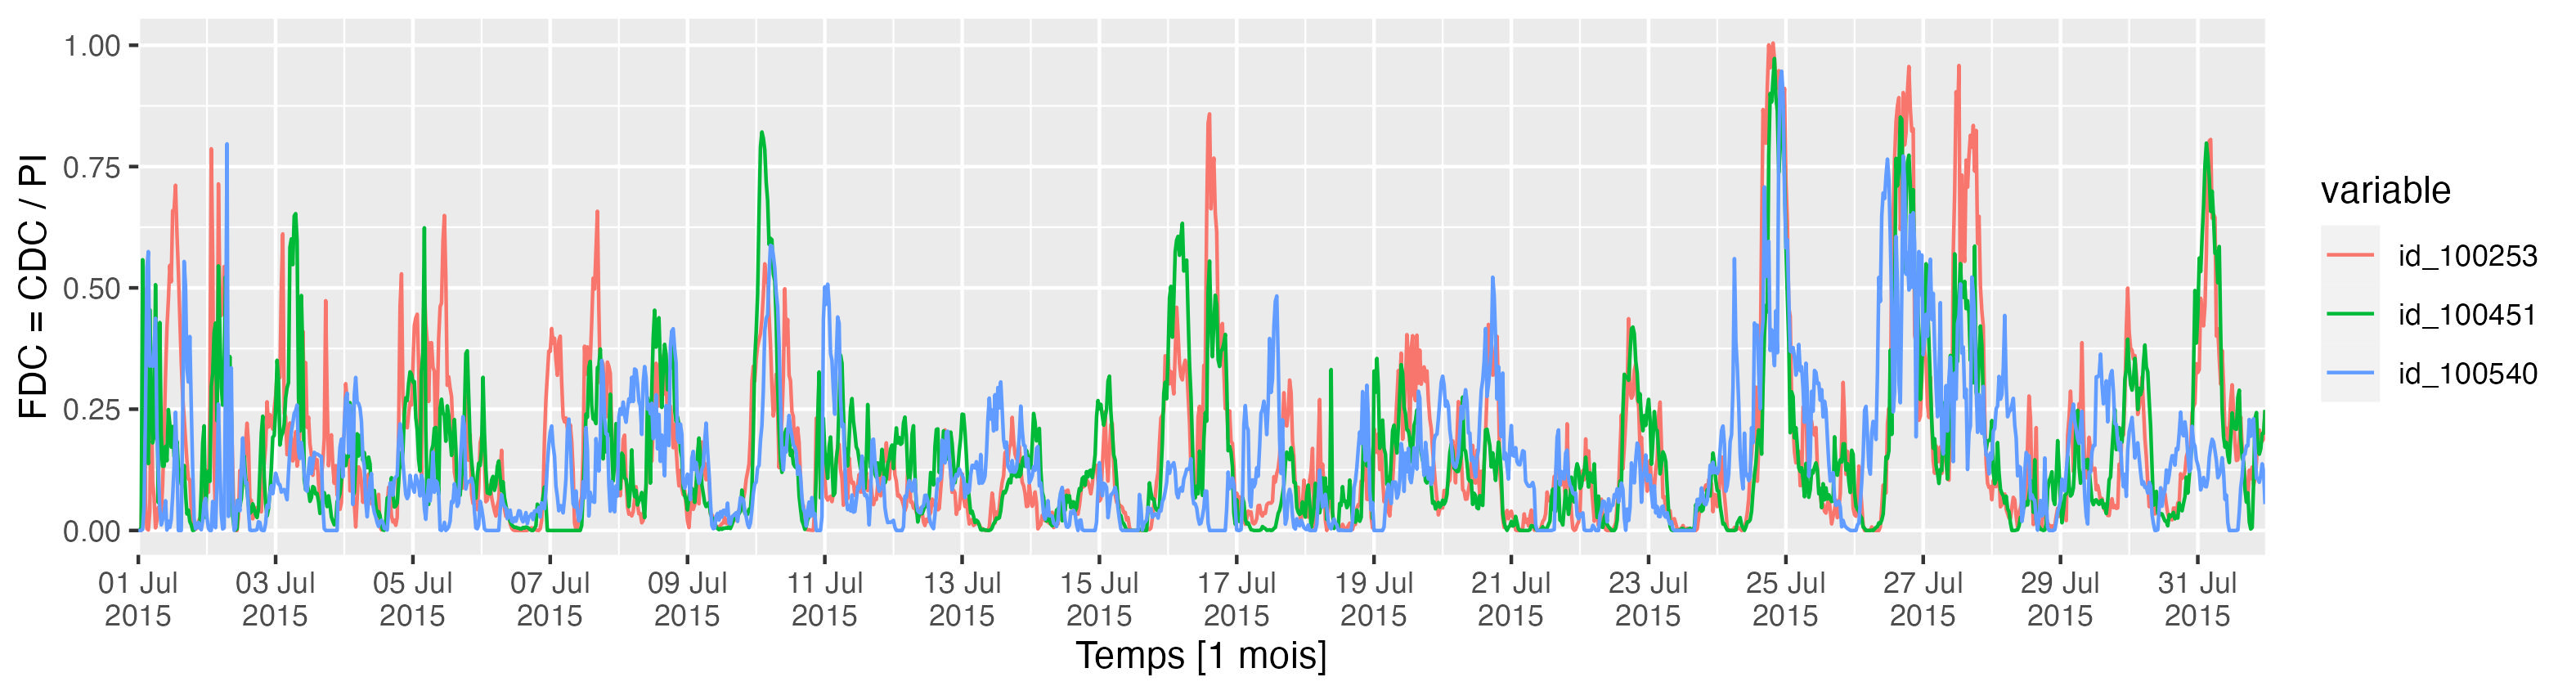
\includegraphics[width=0.85\textwidth]{Images/motivation/test__slice_graph__2015_07__id_1_2_3.jpg}
	}
	\caption{Courbes de charges éoliennes sur 3 premiers parcs éoliens}
	\label{fig:courbes_de_charge}
\end{figure}

\bigskip

Les données qui sont traitées dans le cadre de ce stage sont, entre autres, des courbes de charge observées chaque demie-heure de production électrique éolienne ou photovoltaïque. Le schéma d’observation est donc le \og common-design \fg. C'est-à-dire que les temps d'observations sont ici déterministes à intervalle de temps fixe.

\smallskip

Bien que la différenciation en analyse de séries temporelles soit une méthode efficace pour éliminer la tendance, qu'elle soit saisonnière ou non, permettant ainsi une bonne analyse des données; ces modèles présentent des limites en termes de prédiction à long terme, les rendant moins utiles lorsque l'objectif est de prédire à moyen ou long terme. De plus, ces modèles, ainsi que différents modèles de machine learning populaires, estiment les données courbe par courbe ce qui ne tire pas profit du fait que les observations aient une forme similaire entre les courbes.

\smallskip

Une première idée serait d'utiliser un modèle de série temporelle ARIMA afin de modéliser la dynamique des courbes de charge.


% \book{ \textbf{Un peu d'histoire sur les séries temporelles \ldots}        
\info{une grande partie des informations présentées dans cette section histoire provient de la référience ~\cite{time_series_brief_history} }


\smallskip

Parmi les étapes importantes du développement des séries temporelles, on peut noter l'article \emph{Time Series Analysis : Forecasting and Control} de Box et Jenkins (1970) qui introduit le modèle ARIMA et une approche aujourd'hui standarde d'évaluation du modèle à utiliser ainsi que son estimation. Ce développement est dû en grande partie à l'utilisation de telles données dans les secteurs économiques et des affaires afin de suivre l'évolution et la dynamique de différentes métriques

\smallskip

L'étude des séries temporelle a été divisée en l'étude du domaine fréquentiel, qui étudie le spectre des processus pour le décomposer en signaux principaux, et du domaine temporel, qui étudie les dépendances des indices temporels. L'utilisation de chacune des approches était sujet à débats mouvementés jusqu'aux alentours de l'an $2000$.

\smallskip

Le développement des capacités de calcul a été une révolution notamment pour l'identification des modèles (le critère AIC, l'estimation par vraissemblance dans les années $1980$, \ldots).
% modèles à espace d'états et le filtre de Kalman pour évaluer cette vraissemblance efficacement, MCMC, \ldots).

\smallskip

À partir des années $1980$, les modèles non linéaires émergent (ARCH par Engle, modèles à seuil \ldots) et trouvent application en économie notamment. Enfin l'étude multivariée (modèle VAR) fait surface dans les années 1980 par Christopher Sims~\cite[ \href{https://pubs.aeaweb.org/doi/pdf/10.1257/jep.15.4.101}{lien de l'article} ]{VAR_paper}

\smallskip

Une large partie de la théorie s'appuie notamment sur l'étude des racines de l'unité, en considérant un polynôme d'opérateur $P(B) = (I + \sum_k a_k B^k)$ à partir duquel les relations d'autocorrélations peuvent se ré-écrire.
% }


Toutefois, l'utilisation d'un modèle ARIMA ne permet de modéliser la dynamique du phénomène étudié. En effet, la sélection d'un modèle ARIMA sur le critère du BIC sélectionnait, peu importe le parc éolien, un modèle auto-régressif d'ordre 0. Ainsi le modèle sélectionné considérait les irrégularités de la courbe de charge, dont on attend que le processus duquel elle est issue soit très irrégulier (de par sa complexité), comme étant du bruit. On en conclut que ces modèles peuvent ne pas capturer efficacement la structure complexe des données.

\bigskip

\noindent
\fbox{%
  \parbox{\textwidth}{
    Afin de prédire sur le long terme, nous allons donc adopter une approche basée sur les données fonctionnelles pour capturer la structure de la consommation. Cette approche permettra de d'exploiter une information clé : la similarité entre les courbes observées. 
    }%
}

\question{
	\centering
	\smallskip

	Qu'est-ce qu'une donnée fonctionnelle ?
}

Une donnée est dite fonctionnelle lorsque la variable aléatoire qui nous intéresse n'est plus une variable aléatoire à valeur dans $\mathds R^d$, comme le statisticien a l'habitude de manipuler, mais une variable aléatoire à valeur dans un espace de fonction. Concrètement, chaque réalisation n'est plus un nombre mais bien une courbe toute entière indexée (le plus souvent) sur un intervalle $\mathcal T$.

\begin{figure}[H]
	\centering
	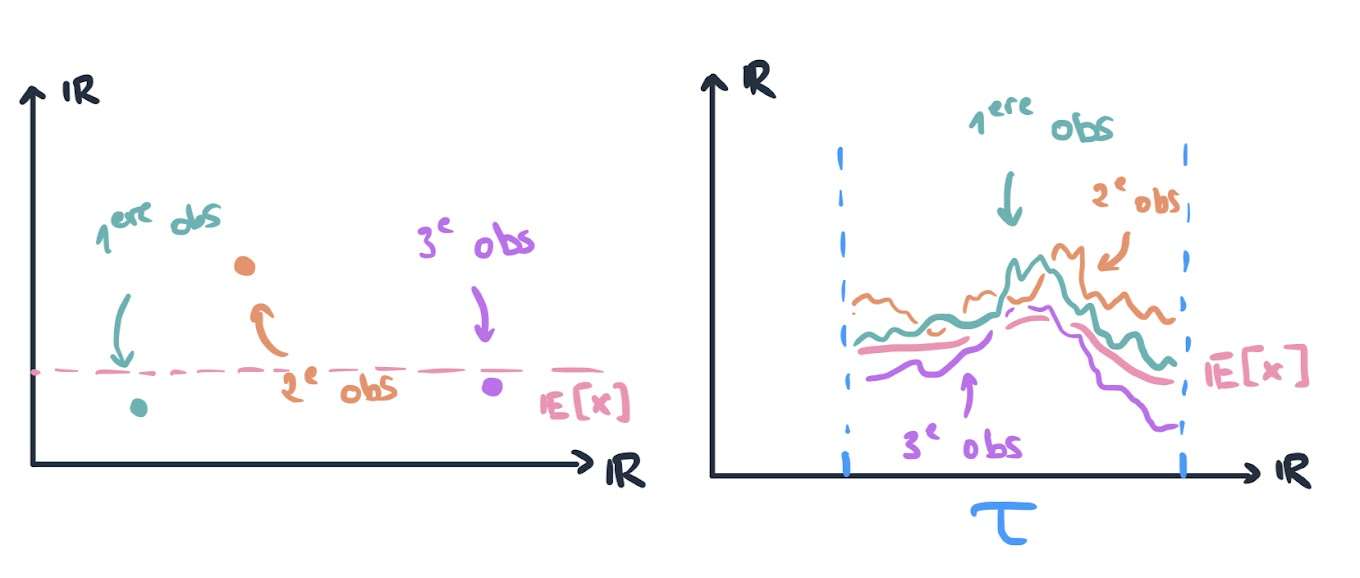
\includegraphics[width=0.85\textwidth]{Images/motivation/donneesRvsFD.jpg}
	\caption{Différence entre donnée fonctionnelle et donnée réelle}
	\label{img:RvsFD}
\end{figure}

Si le statisticien est déjà à l'aise avec l'idée qu'une variable aléatoire réelle identiquement distribuéé puisse modéliser une expérience répétable provenant d'un même phénomène, il pourra se convaincre que les données fonctionnelles permettent elles aussi de modéliser des expériences en lien (fonctionnel) avec un certain paramètre. Et c'est le lien entre les deux valeurs, cette fois-ci, qui provient d'un même phénomène.

\bigskip

Donnons en un exemple : observons la consommation électrique d'un foyer dans une journée. Lorsque l'on travaille sur $\mathds R$, on s'intéresse à sa consommation électrique disons en l'instant $t = 12\mathsf{h}$. Formellement :

\begin{equation*}
	\mathcal T \, \isdef [\, 0,24 \,[ \quad = \textsf{1 jour avec } t \textsf{ en heure}
\end{equation*}

La consommation du foyer $i$ à midi, notée $y_i$, suit la loi d'un phénomène général $Y$, comme une loi normale $\mathcal N\left( 0.27 \, \, kW\mathsf h, 0.1^2 \right)$
%
\footnote{ ordre de grandeur de la consommation électrique d'un foyer en France calculé à partir des données d'ENGIE disponibles librement ~\cite{engie-data-conso-moy-par-an}. \textbf{La variance est arbitraire}, tout comme le choix de la loi juste afin de servir d'exemple. }
%
par exemple. Travailler sur des données fonctionnelles dans ce cadre c'est étudier non plus la consommation $y_i$ à midi, mais regarder l'ensemble de sa consommation en même temps sur toute la journée $y_i(t) = x_i(t)$ avec $t \in \mathcal T$.

\bigskip

On remarque ainsi que toutes les consommations électriques le long de la journée d'un foyer à l'autre suivent la même tendance : on consomme plus le matin avant le travail et le soir alors que pendant la journée on consomme moins car on est au travail. Ainsi c'est la fonction $x_i : \mathcal T \longrightarrow \mathds R$ qui suit la loi d'un phénomène $X$ général. Ce que l'on vient de dire c'est que la \textbf{relation} entre le temps $t \in \mathcal T$ et la consommation électrique ${\, y_i(t) \,}$ est elle même sujet à une loi plus générale. Grossièrement, les courbes auront la même allure, mais chaque individu a sa consommation propre.

\bigskip

\noindent
Plus formellement : comme on a défini une variable aléatoire réelle comme une application :

\begin{equation*}
	\begin{array}{ccc}\Omega &\longrightarrow& \mathds R\\ \omega &\longmapsto& x = X(\omega)\end{array}
\end{equation*}

\noindent
On définit de même une donnée fonctionnelle comme une application :

\begin{equation*}
	\begin{array}{ccc}\Omega &\longrightarrow& \colorize{\mathcal C^0(\mathcal T, \mathds R)}\\ \omega &\longmapsto& x = X(\omega)\end{array}
\end{equation*}

\noindent
Ce que l'on observe sont donc les valeurs des paramètres $t \in \mathcal T$ ainsi que l'image de $t$ par $x$ : $y = x(t)$. Les points que le statisticien observe sont donc les couples de la forme $(t_k^{(\textsf{individu } i)}, y_k^{(\textsf{individu } i)})_{i\in \llbracket 1, m \rrbracket}$, générés par le processus aléatoire $X$ dont la réalisation est la véritable courbe $x_i$ de l'individu $i$ que l'on souhaite estimer pour travailler avec.

\bigskip

\noindent
\info{Il existe différentes façons de définir les données fonctionnelles, une définition possible est la suivante:

	\begin{equation*}
		\begin{array}{ccc}\Omega \times \mathcal T &\longrightarrow& \mathds R \\ ( \omega , t ) &\longmapsto& X(\omega , t) = y\end{array}
	\end{equation*}


	Cependant, cette représentation ne permet pas une interprétation clé en main du concept mais est certainement plus commode à manipuler pour les mathématiciens dans certains contextes. Cette approche est un point de vue de type "processus stochastique" et diffère du point de vue "élément aléatoire" comme traité de façon claire dans ~\cite{HsingEubankTheoreticalFoundationsOfFDA}.
}

\pagebreak

% \book{ \textbf{\ldots et un peu d'histoire sur les données fonctionnelles}
\info{Pour une description plus complète de l'histoire du développement de l'analyse fonctionnelle, on pourra se référer à \href{https://anson.ucdavis.edu/~mueller/fdarev1.pdf}{\textcolor{flatuicolors_blue_deep}{cet article de Wang, Chiou et Müller}}~\cite{wang2016functional}}


Bien que l'histoire du développement de l'Analyse de Données Fonctionnelles (FDA) puisse être retracée jusqu'aux travaux de Grenander et Karhunen~\cite{karhunen1946spektraltheorie} dans les années 1940 et 1950, où l'outil a été utilisé pour étudier les courbes de croissance en biométrie, ce sous-domaine de la statistique a été étudié de manière systématique à partir des années 1980.

\bigskip

En effet, c'est J.O. Ramsay qui a introduit l'appellation de "données fonctionnelles" en 1982~\cite{ramsay1982data} et qui contribuera en partie à sa popularisation. La thèse de Dauxois et Pousse en 1976 sur l'analyse factorielle dans le cadre des données fonctionnelles\cite{dauxois1976analyses} a ouvert la voie à l'analyse par composante principale fonctionnelle (FPCA), un outil clé pour l'étude des données fonctionnelles. La FPCA permet d'étudier des objets fonctionnels qui sont de dimension infinie, difficiles à manipuler et impossibles à observer empiriquement, en dimension finie et surtout sur $\R d$ que l'on connait bien.

\bigskip

Au cours des années 2000, de nombreux outils statistiques déjà développés pour des données à valeurs dans $\R d$ depuis un siècle, tels que la régression linéaire (éventuellement généralisée), les séries temporelles ou encore les modèles additifs, ont été adaptés aux données fonctionnelles.
Par exemple, les modèles de régression linéaire fonctionnelle ont été développés avec une réponse fonctionnelle~\cite{ramsay1991some} ou scalaire~\cite{cardot1999functional} en 1999.
Les modèles linéaires généralisés ont également été étudiés~\cite{james2002generalized,muller2005generalized}, avec l'estimation de la fonction de lien par méthode non paramétrique à direction révélatrice \emph{(Single Index Model)} récemment étudiée en 2011~\cite{chen2011single}.
Cette méthode avait déjà été utilisée en économétrie pour des données de $\R d$ depuis 1963~\cite{sharpe1963simplified}, et leur estimation directe a été étudiée une décennie auparavant par M.Hristache, Juditsky et Spokoiny~\cite{hristache2001direct}. De même, les modèles additifs ont été étendus aux données fonctionnelles en 1999 par Lin et Zhang~\cite{lin1999inference}.
Enfin, le livre de Bosq, \emph{\textcolor{flatuicolors_blue_devil}{Linear Processes in Function Spaces : Theory and Applications}}~\cite{bosq2000linear}, publié en 2000, a contribué au développement des séries temporelles pour les données fonctionnelles.

\bigskip

Depuis lors, des ressources telles que l'ouvrage de Kokoszka et Reimherr, \emph{\textcolor{flatuicolors_blue_devil}{Introduction to Functional Data Analysis (2017)}}~\cite{kokoszka2017introduction}, rendent la théorie et la mise en production des méthodes d'analyse et de prédiction de données fonctionnelles plus accessibles.
% }


\pagebreak


Maintenant que l'on possède une meilleure intuition de ce que sont les données fonctionnelles, il est naturel de se demander pourquoi le choix de modéliser notre phénomène par des données fonctionnelles serait particulièrement judicieux. Pour cela, rappelons nous les difficultés que l'on avait rencontrées dans le cadre de nos données de production électrique en utilisant un modèle de série temporelle classique :

\info{
    \textbf{Rappel : }

    "Ainsi le modèle \colorize{(arima)} sélectionné considérait les irrégularités comme étant du bruit $[\ldots]$ Afin de prédire sur le long terme, nous allons donc adopter une approche basée sur les données fonctionnelles pour capturer la structure de la consommation $[\ldots]$"
}


\question{\smallskip
\centering
    Pourquoi est-ce que l'on s'intéresse autant à la régularité des données que l'on étudie ici ? Et surtout, en quoi est ce que les données fonctionnelles vont nous permettre de mieux capturer la régularité ?
    }

Comme mentionné auparavant, la production électrique est un phénomène très irrégulier [~\ref{fig:courbes_de_charge}] étant influencé par la consommation, la météo, etc. Par conséquent, la prévision de ces courbes de charge doit prendre en compte la nature fondamentalement irrégulière du phénomène afin de proprement le modéliser et, en définitive, mieux le prédire. Ce qui est notamment contraire à la plupart des méthodes qui utilisent des fonctions de classe $\mathcal C^2$ pour lisser les points observés en données fonctionnelles, ce qui limite la prédiction à des courbes de nature $\mathcal C^2$. Cela est d'autant plus critique lorsque l'on cherche à estimer le processus moyen ou l'opérateur de covariance du processus, car ces derniers sont estimés à partir des courbes lissées, qui détruisent toute l'information irrégulière si elle n'est pas prise en compte, impactant significativement l'estimation des objets qui nous intéressent en tant que statisticien.

\editlater{introduire photo qui superpose un mouvement brownien et le lissage spline de ce même mouvement brownien}

Il est ainsi important pour des phénomènes de nature irrégulière de ne pas négliger des précautions lors du lissage afin de ne pas perdre l'information irrégulière. L'idée est donc d'estimer dans un premier temps la régularité de notre processus afin de lisser nos données de manière adaptée pour débruiter et prédire des valeurs non observées tout en préservant les informations irrégulières critiques pour la bonne estimation du processus moyen et de l'opérateur de covariance. L'approche fonctionnelle est clé dans l'estimation de cette régularité, car c'est la \textbf{réplication de courbes} de même nature qui permet in-fine d'\textbf{estimer la régularité} du phénomène.

% ~ ——————————————————————————————————————————————————————————







\chapter{Méthodologie}
\minitoc%

\section{Données Fonctionnelles : l'essentiel}

    \subsection{Définitions et propritétés informelles}


Commençons par introduire les données fonctionnelles de manière informelle afin de mieux intégrer la définition formelle, plus utile pour la manipulation.

Cette section regroupe l'ensemble des messages essentiels à retenir des données fonctionnelles pour la pratique, sans alourdir les notions avec des notations mathématiques. Le cadre formel sera traité juste après.

\begin{definition*}[données fonctionnelles — informel]
    Les données fonctionnelles sont des données dont les observations sont des fonctions, c'est-à-dire des courbes, des surfaces, des images, \, \dots
    
    i.e : toute donnée ayant une dépendance de type "relation fonctionnelle" avec un ou plusieurs paramètres.
    \label{def*:fda}
\end{definition*}

\begin{figure}[H]
    \begin{center}
        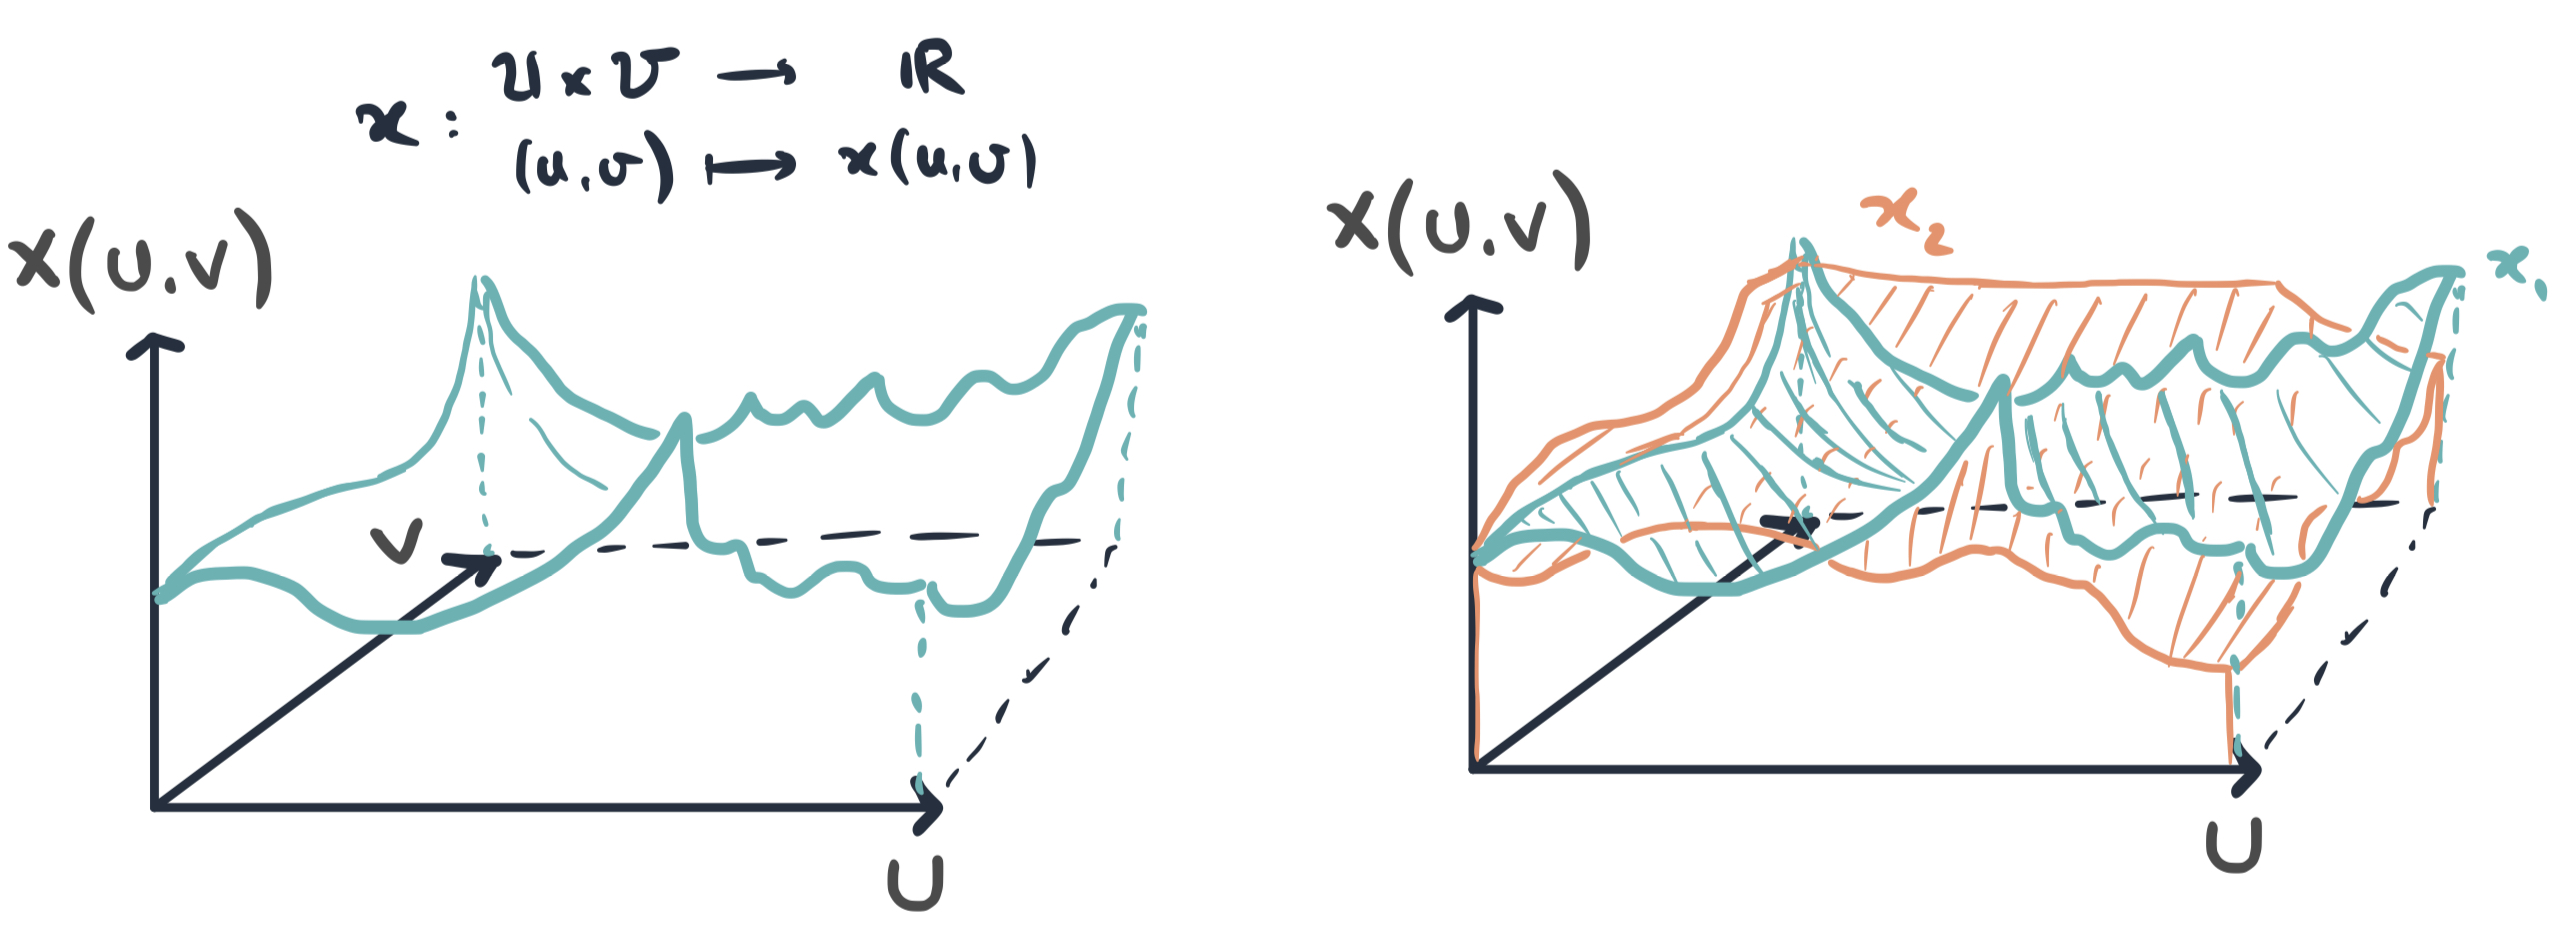
\includegraphics[width=\textwidth]{Images/sketches/fda_surface.jpg}
    \end{center}
    
    {
    \textbf{Gauche :} exemple de surface
    \\
    \textbf{Droite :} échantillon de deux observations de la surface suivant une loi fonctionnelle}

    \caption{Donnée fonctionnelle : relation fonctionnelle avec plusieurs paramètres}
    \label{fig:sketch_surface}
\end{figure}

Maintenant introduites, les théorèmes suivant permettent de manipuler ces données à la fois pour la théorie et la pratique :

\begin{thm*}[\nameref{thm:KL} — informel]
    \noindent\fbox{%
    \parbox{\textwidth}{%
    Il est possible pour une large classe de données fonctionnelles de les décomposer dans une base \emph{de fonctions} adaptée aux données (au sens de la covariance) que l'on appelle base ACP fonctionelle (FPCA).
    }%
    }
    \label{thm*:KL}
\end{thm*}
\begin{proof}[\faCogs \, preuve informelle]
    La covariance est un opérateur bilinéaire symétrique défini positif, on peut donc appliquer le théorème de Mercer (équivalent du théorème spectral) qui nous donne une base orthonormale de $\mathds L^2$ sur laquelle on va décomposer notre processus \textbf{centré}.
\end{proof}
\begin{rem}
    La classe de fonctions pouvant être décomposées est large, puisqu'elle regroupe l'ensemble des processus qui nous intéressent la plus part du temps en tant que statisticien : celles qui sont à support sur un intervalle, admettant une covariance continue et finie sur le support.
\end{rem}
    
On en déduit que pour travailler avec des données fonctionnelles, il suffit de les décomposer dans la base ACP fonctionnelle puis de travailler sur les composantes de chaque élément de la base. On travaille désormais avec des réels et non plus des fonctions, ce qu'on aime manipuler. On peut alors faire de la statistique traditionnelle avec les outils que l'on connait.


\begin{propriete*}[intérêt de la base FPCA — informel]
    \noindent\fbox{%
    \parbox{\textwidth}{%
    la base ACP fonctionnelle est la plus économe, c'est à dire qu'elle explique au mieux la covariance des données pour un nombre de composantes fixées, ce qui est utile car on ne sait manipuler numériquement que des objets de dimension finie.
    }%
    }
\end{propriete*}

\subsection{estimation adaptative informelle}

On a mentionné qu'il serait judicieux de lisser les observations en tenant compte de la régularité du processus dont est issu nos données. La question est désormais la suivante :

\question{
    Est-il possible de récupérer la régularité locale des trajectoires à partir des données ? Si oui, comment ?
}

C'est ce qu'affirme le théorème suivant à partir des travaux de Golovkine et al. ainsi que Maissoro-Patilea-Vimond (MPV) :

\begin{thm*}[Regularité locale — informel]
    \noindent\fbox{%
    \parbox{\textwidth}{%
    Les données fonctionnelles permettent de récupérer la régularité locale des trajectoires. Les estimateurs définis \textbf{ponctuellement} convergent. 
    }%
    }
    \label{thm*:regularite_locale}
\end{thm*}
\begin{rem}[Continuité de Kolmogorov]
    Un théorème (\nameref{thm:kolmogorov_continuite}) permet à partir de l'espérance d'incréments d'un processus aléatoire de déduire sa régularité.
    C'est pourquoi les estimateurs sont définis à partir de l'espérance des incréments quadratiques du processus. C'est entre autres \emph{la raison pour laquelle les données fonctionnelles permettent de récupérer la régularité locale des trajectoires}.

    \label{rem:kolmo_continuite}
\end{rem}

Les motivations de l'obtention de la régularité étaient en partie de pouvoir mieux estimer les quantités qui nous intéressent dont la fonction moyenne du processus, ainsi que son opérateur de covariance. Ce qui est à la fois important pour l'analyse (via l'interprétation de la base ACP déterminée par la covariance) et pour la prédiction. On peut alors se demander si il existe des estimateurs de la moyenne et de la covariance prenant en compte la régularité locale. C'est ce qu'affirme les théorèmes suivants :

\warn{demander à Hassan la dernière version de son papier car la partie d estimation adaptative a beaucoup changé}

\begin{thm*}[Estimateurs de la moyenne et de la covariance — informel ~\cite{golovkine2021adaptive}]
    \noindent\fbox{%
    \parbox{\textwidth}{%
    Il est possible en lissant les observations par méthode à noyaux avec une largeur de bande \emph{spécifique à l'objet que l'on souhaite estimer}, de dériver des estimateurs de la moyenne et de la covariance qui convergent. 
    La largeur de bande optimale \emph{pour l'objet que l'on souhaite estimer} est celle qui minimise un risque qui effectue un compromis biais-variance, qui dépend de la régularité locale du processus, en pénalisant les largeurs de bande menant à des "trous" dans les fonctions lissées.
    On parle d'\emph{\og estimation adaptative \fg}.
    }%
    }

    \label{thm*:estimation_adaptative}
\end{thm*}

Cependant, bien qu'une largeur de bande optimale existe, elle est inconnue. Il est donc important de savoir si le praticien peut l'estimer, et avec quelle précision (c'est à dire à quel point l'estimateur sera biaisé ou non). C'est ce que nous affirme le théorème suivant :

\pagebreak

\begin{thm*}[expression de la largeur de bande optimale — informel ~\cite{golovkine2021adaptive}]
    \noindent\fbox{%
    \parbox{\textwidth}{%
    Sous certaines hypothèses de régularité du processus, et d'indépendance des temps observés, la largeur de bande optimale peut être approchée (avec forte probabilité de bonne approximation) par une expression ne dépendant que du nombre de courbes observées, du nombre moyen de temps observés par courbe, et de la régularité locale du processus. Ce biais de l'estimateur de la fonction moyenne est alors contrôlé en fonction de ces mêmes quantités.

    Sous des hypothèses un peu plus fortes sur le nombre d'observations par courbe, et le nombre de courbe on dispose de résultats similaires pour l'estimateur de la covariance.}%
    }
        
    \label{thm*:h_opt_estim}
\end{thm*}


Enfin, on peut se demander ce qu'il en est des estimateurs dans le cadre où l'on dispose de la dépendance dans les données (ce qui est la cas pour les données éoliennes notamment). Ce cas est traîté par le théorème suivant dérivé par MPV :

\begin{thm*}[ Estimation adaptative de séries temporelles fonctionnelles — informel ~\cite{maissoro-SmoothnessFTSweakDep} ]

    On peut estimer la régularité d'une série temporelle de données fonctionnelles à condition que la mémoire temporelle de la série soit courte. (La décroissance de la dépendance temporelle doit être au moins aussi rapide qu'une décroissance géométrique)

    \label{thm*:far_adaptative_estimation}
\end{thm*}

\pagebreak

\subsection{Résumé informel de la méthodologie}

Les données fonctionnelles permettent de travailler sur un modèle où la \emph{relation} entre plusieurs quantités est sujet à une loi \colorize[flatuicolors_biscay]{[$cf$ \nameref{def*:fda}]}. Ce point de vue de réplication de courbes est notamment utile car il permet d'extraire des observations leur régularité \colorize[flatuicolors_biscay]{[$cf$ \nameref{rem:kolmo_continuite}, \nameref{thm*:regularite_locale}]}. L'estimation de cette régularité permet, entre autres, de lisser les courbes de façon appropriée en fonction de la quantité que l'on souhaite estimer, telle que la moyenne et la covariance avec une plus grande précision \colorize[flatuicolors_biscay]{[$cf$ \nameref{thm*:estimation_adaptative}]}. 

\noindent\begin{figure}[H]
    \centering
    \pagewidthimg{Images/sketches/sketch_resume_informel.jpg}
    \caption{Résumé des motivations du de l'estimation de la régularité locale des trajectoires}
    \label{fig:sketch_resume_informel}
\end{figure}


\pagebreak

\subsection{Données fonctionnelles : formellement}

\subsubsection{Définition formelle}

Pour éviter d'alourdir les notations, on se place dans le cas où les fonctions sont à valeurs dans $\mathds R$ et à support sur un intervalle fermé $I$ de $\mathds R$. Toutefois, on peut très bien considérer des fonctions à valeurs dans $\mathds R^d$ et à support sur un compact $K$ de $\mathds R^p$ sans perte de généralités.

\begin{definition}[données fonctionnelles ]

    On appelle données fonctionnelles, un échantillon $\famfinie x 1 n$ de fonctions continues $x_i : I \rightarrow \R d$ issues d'un processus $X$ défini comme ci-dessous :

    $$X : 
    \begin{array}{ccc}
        \Omega & \longrightarrow & \mathcal C(I, \mathds R)
        \\
        \omega & \longmapsto & X(\omega) = x 
    \end{array}
    $$

\end{definition}

\subsubsection{Résultats importants}

On énonce désormais le théorème central de l'analyse de données fonctionnelles qui n'est autre que la décomposition dans la base FPCA de notre processus.

\begin{rem}
    on notera que dans le cadre des données fonctionnelles, on ne travaille pas de façon générale avec la covariance :
    
    $$C_X : (s,t) \mapsto \esperance{ (X - \mu)(s) \cdot (X - \mu)(t) }$$
    
    On travaille plutôt avec l'\textbf{opérateur} de covariance :
    $$f \mapsto \int\limits_I f(u)C_X(u, \cdot \,) \,du$$ 
    
    C'est parceque cet opérateur est linéaire continu (car Hilbert-Schmidt donc borné pour la norme d'opérateur) symétrique semi-défini positif (pour le produit scalaire de $\mathds L^2$) et que l'on peut donc en faire une décomposition spectrale sur une base orthonormale de vecteurs propres associés à des valeurs propres positives. Cette décomposition est à la base des approximations que le praticien effectuera ainsi qu'à la base de la dérivation de nombreux théorèmes et propriétés.
\end{rem}

\bigskip

Etant donné que l'on traîte des données fonctionnelles, on considère la géométrie usuelle de $\mathds L^2(\mathds R, \, \lambda)$ et on note ainsi 

$$\prodscalselon \cdot \cdot {\mathds L^2}: \begin{array}{ccc}
    \mathds L^2 \times \mathds L^2 & \longrightarrow & \mathds R
    \\
    (f,g) & \longmapsto & \int f(u)g(u) \, d\lambda(u) 
\end{array}$$ 

le produit scalaire que l'on considère pour manipuler les données fonctionnelles.

% https://stackoverflow.com/a/4008463 : no page break
\begin{minipage}{\textwidth}
\begin{thm}[Karhunen-Loeve]
    \emph{référence :} ~\cite[pages : 238-239-241]{kokoszka2017introduction}

    \textbf{Hypothèses :}

    $$
    \boxed{
    \begin{array}{ll}
        \textsf{\faCaretSquareRight} & X \in \mathds L^2( \Omega, \mathcal C(I, \mathds R)) 
        \\ \\
        \textsf{\faCaretSquareRight} & \textsf{covariance : } C : \begin{array}{ccc}
            \mathds L^2( \Omega, \mathcal C(I, \mathds R)) & \longrightarrow & \mathcal C(I^2, \mathds R)
            \\
            X & \longmapsto & C_X
        \end{array}
        \\ \\
        & \textsf{ie : } C_X : (s, t) \mapsto C_X(s,t) \textsf{ est continue}
        \\ \\
        \textbf{\faIcon{asterisk}} & \textsf{opérateur covariance} \, c_X[ \, \cdot \, ] : \begin{array}{ccc}
            \mathcal C(I, \mathds R) & \longrightarrow & \mathcal C(I, \mathds R)
            \\
            f & \longmapsto & \int_I f(s) C_X(s, \cdot \, ) \, ds \end{array}
        \\\\
        \textsf{\faCaretSquareRight} & \textsf{valeurs propres ordonnées : } \forall p \geq 1, \lambda_{p+1} \leq \lambda_p \quad\quad \lambda_p, \lambda_{p+1} \in \operatorname{sp}(c_X)
        \\ \\
        \textbf{\faIcon{asterisk}} & \textsf{on pose } \overrightarrow{sp}_{\orthonormal}^{[1,p]}(c_X) \isdef \left\{ \phi_k \in \overrightarrow{sp}_{\orthonormal}( \, c_X \, ) \textsf{ associé à }  \lambda_k, k \in \intervaleint 1 p \, \right\}
    \end{array} 
    }
    $$

    \textbf{alors :}
    $$
    \boxed{
    \begin{array}{cc}
        \textsf{\faCaretSquareRight} & 

            \forall p \geq 1 
            \quad
            \argmin\limits_{u_k \in \mathcal C(I, \mathds R)} \mathds E \left\Vert X - \sum\limits_{k=1}^p \prodscalselon {X - \mu} {u_k} {\mathds L^2} u_k \right\Vert^2 = \overrightarrow{sp}_{\orthonormal}^{[1,p]}( \, c_X \, )

        \\
        \\
        \textsf{\faCaretSquareRight} & X = \mu + \sum\limits_{k=1}^{+\infty} \prodscal {X - \mu} {\phi_k} \phi_k
        \\
        &
        \\
         &\textsf{avec } \phi_k \in \overrightarrow{sp}_{\orthonormal}( \, c_X \, )
    \end{array}
    }
    $$

    \label{thm:KL}
\end{thm}
\end{minipage}

\begin{rem}
    pour pouvoir ordonner les valeurs propres dans l'ordre décroissant, et sélectionner les composantes principales les plus informatives, il faut pouvoir réarranger l'ordre de la somme. Pour cela il faut que les valeurs propres forment une famille sommable, une condition suffisante et souvent utilisée est que $\mathds E \Vert X \Vert^2 < \infty$ 
\end{rem}

\begin{rem}
    la propriété de la section précédente sur l'aspect économe de la base FPCA découle directement de l'assertion $\forall p \geq 1 
    \quad
    \argmin\limits_{u_k \in \mathcal C(I, \mathds R)} \mathds E \left\Vert X - \sum\limits_{k=1}^p \prodscal {X - \mu} {u_k} u_k \right\Vert^2 = \overrightarrow{sp}_{\orthonormal}^{[1,p]}( \, c_X \, )$ dans le théorème de Karhunen-Loeve.
\end{rem}




    \subsection{Cas non indépendant : séries temporelles de données fonctionnelles}
        
    Une large partie de la théorie des données fonctionnelles suppose que l'on observe des courbes $X_i : \Omega \rightarrow \mathcal C^0(I, \mathds R)$ \textbf{indépendantes} et identiquement distribuées. Cependant une partie non négligeable des données que l'on observe ont des dépendances avec les valeurs passées. Par exemple, il est raisonnable de penser que la consommation électrique d'un foyer au cours d'une année croît avec l'ajout successif de nouveau appareils électroniques. L'hypothèse d'indépendance entre les données n'est donc plus pertinente pour les données que l'on traite et il devient important de considérer des processus autorégressifs adaptés aux données fonctionnelles. 
Si dans le cadre des données de $\mathds R$ cette relation de \emph{dépendance linéaire} avec le passé pouvait s'écrire sous la forme suivante 
$X_n = \sum\limits_{k=1}^{n-1} \varphi_k \, X_k + \varepsilon_n$ où $\varphi_k \in \grandR$ 
et 
$\varepsilon_n \begin{cases} \in \operatorname{VA}(\grandR) \\ \indep \sigma\left( X_i \right)_{1\,: \, n-1}\end{cases}$, 
dans le cadre fonctionnel on capture la même idée en considérant 
$X_n = \sum\limits_{k=1}^{n-1} \phi_k \left( X_k \right) + \varepsilon_n$ où $\phi_k$ 
est un \emph{opérateur linéaire} de $\mathds L^2(I, \mathds R)$, 
le plus souvent intégral. 

\chk{
    Il s'agit d'une généralisation naturelle de la relation dans le cadre réel, puisqu'on peut démontrer que sur l'espace des nombres réels l'ensemble des fonctions linéaires $\phi : \grandR \rightarrow \grandR$ sont de la forme $x \mapsto ax$ avec $a \in \grandR$. La relation sur $\grandR$ que l'on a vue juste avant peut alors se ré-écrire de façon similaire à la version fonctionnelle.
    }

On considère lors de ce stage des séries temporelles de données fonctionnelles car les données que l'on manipule ( en l'occurence les données de courbe de charge des parcs éoliens ) semble être naturellement corrélées dans le temps. 

\warn{Il faut cependant faire attention avec l'interprétation de séries temporelles fonctionnelles. En effet l'interprétation que l'on fait d'une série temporelle fonctionnelle ne peut être véritable calquée sur l'interprétation dans la cadre réel. 

\quad Si sur $\mathds R$ la corrélation temporelle s'interprête comme le fait que l'observation suivante (c'est à dire le facteur de charge du parc éolien) dépend de l'observation précédente (c'est à dire dépend du jour précédent par exemple), dans le cadre fonctionnel l'observation est une fonction. On rappelle que dans le cadre des données éoliennes, chaque observation est la courbe de charge observée su un an. Ce que cela signifie, c'est que la dépendance à l'observation passée que l'on va constater sur l'observation suivante n'affecte pas un unique point. Elle affecte tous les points de la courbe de charge simultanément. La dépendance temporelle concerne l'année entière, d'une année à l'autre. Fixer le $t$ dans $X_n(t)$ ne garantit pas l'observation de la même structure de dépendance comparé à la série temporelle fonctionnelle. 

\quad Par exemple, en utilisant un opérateur intégral pour $\phi_k$, comme $\phi_k :X \mapsto \int_I  \beta_k(u,t) X(u) du$, la vision de regarder les $t$ individuellement et de regarder leur évolution selon les années n'est pas évidente à interpréter car $\phi_k(X)$ intègre des informations de $X$ sur l'ensemble des $t \in I$, dû à l'intégrale.}

\pagebreak

\section{Estimation de la régularité locale des trajectoires}

\subsection{Ce qu'on entend par régularité locale}


Longtemps, il était cru que les fonctions continues étaient dérivables presque partout. C'est notamment Weierstrass qui a démontré qu'il existe des fonctions continues partout mais dérivable nulle part. Poincaré notamment disait de tels objets qu'ils n'existaient que pour contredire le travail des pères. 
Cependant, des objets manipulés tous les jours comme le monde de la finance notamment traitent des processus qui sont fondamentalement irréguliers
%
\footnote{les fonctions dérivables nulle part sont même denses dans les fonctions continues pour la topologie de la convergence uniforme~\cite{gourdon2020maths-dense-non-deriv}. A epsilon près on rencontre toujours une fonction dérivable nulle part lorsque l'on considère la distance maximale réalisée entre deux fonctions continues sur leur support $I$...}
%
(au point de vue de l'analyse, où l'on traite souvent des fonctions au moins dérivables). Il est donc important de pouvoir quantifier la régularité d'une fonction de façon plus fine que le nombre de dérivées qu'elle possède. 

Nous allons repasser rapidement en revue les différents concepts de régularité pour mettre l'emphase dans ce que l'on considère comme régularité locale.

Afin de savoir à quel niveau de régularité nous souhaitons estimer, il est important de garder en tête un ordre de différents niveaux de régularité résumé par les relations suivantes :

$$\textsf{Lipschitz} \implies \textsf{Hölder} \implies \underbracket{\colorize{\textsf{Localement Hölder}}}_{\textsf{ce qui nous intéresse}} \implies \textsf{Uniformément continue} \implies \textsf{Continue}$$

Afin de mieux discerner ce que chaque propriété signifie, et quelles sont les différences entre chaque niveau de régularité, nous allons rappeler rapidement les définitions de ces propriétés.

\begin{itemize}
    \item Continuité :
    $$(\forall \varepsilon > 0) \, (\forall x) (\exists \delta_{\colorize x} > 0) (\forall y) \, |x-y| < \delta \implies |f(x) - f(y)| < \varepsilon$$
    \item Uniforme Continuité :
    $$(\forall \varepsilon > 0) \, (\exists \delta > 0) (\forall x,y ) \, |x-y| < \delta \implies |f(x) - f(y)| < \varepsilon$$

    \item Lipschitz :
    $$\exists L_I \quad(\forall x,y \in I) \quad |f(x) - f(y)| < L_I |x-y|$$
    \item Hölder :
    $$
    \exists \alpha \in (0,1] \quad \exists L_{\alpha(I)} \quad (\forall x,y \in I) \quad |f(x) - f(y)| < L_{\alpha(I)} |x-y|^\alpha
    $$
    \brain{
    une fonction lipschitz est une fonction Holderienne avec $\alpha = 1$
    }

    \item Localement Hölder :
    $$
    \forall x_0 \in I \quad \exists \alpha\left(x_0\right), L_{\alpha(x_0)}\left( x_0\right) \quad \begin{cases}
    (\forall x) \quad |f(x) - f(x_0)| < L_{\alpha(x_0)} |x-x_0|^{\alpha(x_0)}
    \\
    \quad 0 < {\alpha(x_0)} \leq 1 
    \end{cases}
    $$
\end{itemize}

\question{
    \smallskip\centering
    Pourquoi se concentrer sur des processus localement Hölder ?
}

La nature des phénomènes rencontrés dans la vie réelle est souvent complexe. Influencés par de nombreux phénomènes, certains d'entre eux sont, comme mentionnés précédemment, irréguliers. C'est notamment le cas des courbes de charge électriques, qui dépendent de multitudes de phénomènes physiques ou comportementaux, dont on peut attendre une certaine régularité, mais qui ne sont pas nécessairement uniformes tant sur leur niveau régularité que l'intervalle de temps sur lequel ils ont une influence. On pourrait par exemple attendre une différence de régularité de la production électrique en plein été (soleil et température stables \ldots) comparé au mois de mars (plus grande instabilité des conditions climatiques).

De plus, les fonctions Hölderiennes représentent une classe suffisamment large de fonctions. 
% \editorwarn{citer le papier sur le fractional brownian motion (how large)}
L'espace de fonctions sur lequel on travail est donc devrait être en pratique suffisamment grand pour inclure l'ensemble des processus qui nous intéressent. Enfin les fonctions que le praticien sera amené à manipuler seront des fonctions d'un intervalle dans $\mathds R$, qui lorsque continues sont automatiquement uniformément continues en vertu du théorème de Heine. Il est donc naturel de se concentrer sur des fonctions localement Hölderiennes. \footnote{Afin de ne pas alourdir l'essence du propos, une simplification par rapport à l'article de MPV~\cite{maissoro-SmoothnessFTSweakDep} a été faite, si le lecteur souhaite aller dans le détail, il est possible de se référer à l'Annexe \ref{annexe:regularite-locale}.}


\subsection{Estimation des paramètres régularité locale des trajectoire}

\subsubsection{Deux méthodes d'obtention de la régularité locale des trajectoires}

Il existe deux méthodes différentes pour estimer la régularité des trajectoires. Si la clé des deux méthodes pour extraire la régularité locale est le théorème de continuité de Kolmogorov énoncé ci-dessous, les deux méthodes diffèrent par les points $t \in \mathcal T$ considérés dans l'estimation des accroissements quadratiques $\esperance{ \vert X(u) - X(v) \vert^2 }$ utilisés pour l'estimation de la régularité locale. 

\begin{thm}[Continuité de Kolmogorov]
    \emph{référence : } ~\cite[thm : 2.197 | page : 145]{capasso2015introduction}

    $$
    \begin{array}{ll}
        \textsf{\faCaretSquareRight} 
        & X : \, \begin{array}{ccc}
            \mathbb{R_+} \times \Omega & \longrightarrow & \mathbb{R} \\
            (t, \omega) & \longmapsto & X(t, \omega) = x(t)
            \end{array} \textsf{séparable}
        & &
        \\
        \textsf{\faCaretSquareRight}
        & \exists r,c, \varepsilon, \delta \in \mathds R_+ \quad (\forall h < \delta)(\forall t \in \mathds R_+)  \quad \esperance{ | X(t+h) - X(t) |^r } \leq c\cdot h^{1+\varepsilon}
    \end{array}
    $$
    \begin{center}
        $\Downarrow$
    \end{center}
    $$ 
    \textbf{\faIcon{asterisk}}\, \boxed{
        X \textsf{ est continu en } t \in \mathds R_+ \textsf{ pour presque tout } \omega \in \Omega
    }
    $$
    \begin{center}
        ie : il existe une version $\tilde X$ de $X$ continue en $t$ telle que $\proba{ \tilde X(t) = X(t)} = 1$
    \end{center}

    $$
    \textbf{\faIcon{asterisk}} \, \boxed{
        \tilde{X} \textsf{ est } \gamma \textsf{-Hölderienne en } t  \textsf{ pour tout } 0 < \gamma < \frac{\varepsilon}{r}
    }
    $$
    \label{thm:kolmogorov_continuite}
\end{thm}

Etant donné que notre estimateur utilise les incréments quadratiques, on se place dans le cas où $r = 2$.

% \editorwarn{Mettre la version avec Hölder, qui permet de dériver des fda la régularité locale}


La méthode de Golovkine et al. ~\cite[pages : 7—9]{golovkineRegularityOnlineEstimationNoisyCurve} n'utilise que les points observés, et construit un estimateur des incréments quadratiques à base de statistique d'ordre. 

$$\theta( T_{(l)}, T_{(k)}) = \esperance{ \left| X( T_{(l)}) - X(T_{(k)}) \right|^2 }  \begin{align*}
    &\quad \underset {\textsf{LGN}} \approx 
    & \boxed{\frac 1 {N} \sum\limits_{n=1}^N \left| \statrang Y n {2k-1} \statrang Y n k \right|^2 \isdef \hat \theta_k}
    \\
    & \, \underset {+ \mathcal C^0 Kol.} {\overset {\textsf{Hölder}} \approx}
    & L_{t_0} \esperance{| \ordered T l - \ordered T k |^{2H_{t_0}}} 
    & \rightarrow H_{t_0} = f(\theta)
\end{align*}  $$

$$\hat H_{t_0}(k) = \begin{cases} \displaystyle\frac{\log\left( \hat \theta_{4k-3} - \hat \theta_{2k-1}  \right) - \log \left(  \hat\theta_{2k-1} - \hat \theta_k \right)}{2\log 2} & \hat \theta_{4k-3} > \hat \theta_{2k-1} > \hat \theta_{k}
    \\
    1 & \textsf{sinon}
\end{cases}$$

\info{Cette méthode peut s'avérer spécifiquement utile lorsque l'on traite un flux de données, car l'arrivée de nouvelles données ne nécessite pas spécifiquement de recalculer les incréments quadratiques sur l'ensemble des points observés. }

L'autre méthode proposée par ~\cite{golovkine2021adaptive,maissoro-SmoothnessFTSweakDep}, elle se base sur l'utilisation de points non observés, inférés par lissage des courbes, à une distance $\Delta / 2$ les uns des autres pour estimer les incréments quadratiques. Cette dernière méthode implique le choix d'un hyper-paramètre lors de l'estimation $\Delta$ et pourrait être sensible à la qualité du lissage de la courbe. Etant donné que l'objectif de la détermination de la régularité locale est de pouvoir faire un lissage à noyaux adaptatif en fonction de l'objet que l'on souhaite estimer, on appelle le lissage effectué pour estimer la régularité \og pré-lissage \fg.

% https://tex.stackexchange.com/questions/156993/plotting-weierstrass-function
\begin{figure}[H]
    \centering
    \begin{minipage}{0.45\linewidth}
        \begin{tikzpicture}
    \pgfmathsetmacro{\pgfdeltavalue}{0.25}
    \pgfmathsetmacro{\pgftvalue}{0.4}
    \pgfmathsetmacro{\pgfarrowheight}{-0.25}
    \pgfmathsetmacro{\pgfarrowfrom}{\pgftvalue - \pgfdeltavalue/2}
    \pgfmathsetmacro{\pgfarrowto}{\pgftvalue + \pgfdeltavalue/2}
    \begin{axis}[axis lines=middle,
        xmin=0, xmax=1,
        ymin=-0.4, ymax=0.4,
        axis equal image,
        ytick=\empty,
        xtick=\empty,
    ]
    \addplot [flatuicolors_green, samples=300, domain=0:1.1] {weierstrass(2*x,2,15)};

    \addplot [flatuicolors_imperial, mark=*, only marks] coordinates {(\pgftvalue, {weierstrass(2*\pgftvalue,2,15)})};
    \addplot [flatuicolors_imperial, mark=*, only marks] coordinates {(\pgftvalue - \pgfdeltavalue/2, {weierstrass(2*(\pgftvalue - \pgfdeltavalue/2),2,15)})};
    \addplot [flatuicolors_imperial, mark=*, only marks] coordinates {(\pgftvalue + \pgfdeltavalue/2, {weierstrass(2*( \pgftvalue + \pgfdeltavalue/2 ),2,15)})};

    \addplot[color=flatuicolors_imperial,mark=none, thick, dashed] (\pgftvalue + \pgfdeltavalue/2,x);
    \addplot[color=flatuicolors_imperial,mark=none, thick, dashed] (\pgftvalue - \pgfdeltavalue/2,x);
    \addplot[color=flatuicolors_imperial,mark=none, thick, dashed] (\pgftvalue,x);

    \draw[color=white, fill=white] (\pgftvalue - 0.005, \pgfarrowheight - 0.05 - 0.025) rectangle (\pgftvalue + 0.005, \pgfarrowheight - 0.05 + 0.025);
    \node at (axis cs: \pgftvalue, \pgfarrowheight - 0.05) {$\colorize[flatuicolors_aqua]{ \mathbf \Delta}$};

    \draw[flatuicolors_aqua, ->] (axis cs:\pgfarrowfrom, \pgfarrowheight) -- (axis cs: \pgfarrowto, \pgfarrowheight);
    \draw[flatuicolors_aqua, <-] (axis cs:\pgfarrowfrom, \pgfarrowheight) -- (axis cs: \pgfarrowto, \pgfarrowheight);
        
    \draw[color=white, fill=white] (\pgftvalue - 0.05, -0.06) rectangle (\pgftvalue + 0.05,-0.005);
    \node at (axis cs: \pgftvalue,  -0.03 ) {$\colorize[flatuicolors_imperial]{ t_2}$};
    \draw[color=white, fill=white] (\pgftvalue - \pgfdeltavalue/2 - 0.05, -0.06) rectangle (\pgftvalue - \pgfdeltavalue/2 + 0.05,-0.005);
    \node at (axis cs: \pgftvalue - \pgfdeltavalue/2 -0.01,- 0.03) {$\colorize[flatuicolors_imperial]{ t_1}$};
    \draw[color=white, fill=white] (\pgftvalue + \pgfdeltavalue/2 - 0.005, 0.005) rectangle (\pgftvalue + \pgfdeltavalue/2 + 0.005, 0.08);
    \node at (axis cs: \pgftvalue + \pgfdeltavalue/2, 0.04 ) {$\colorize[flatuicolors_imperial]{ t_3}$};
    
    \end{axis}

\end{tikzpicture}

    \end{minipage}
    \hfill
    \begin{minipage}{0.45\linewidth}
        \begin{tikzpicture}
    \pgfmathsetmacro{\pgfdeltavalue}{0.25}
    \pgfmathsetmacro{\pgftvalue}{0.15}
    \pgfmathsetmacro{\pgfarrowheight}{-0.25}
    \pgfmathsetmacro{\pgfarrowfrom}{\pgftvalue - \pgfdeltavalue/2}
    \pgfmathsetmacro{\pgfarrowto}{\pgftvalue + \pgfdeltavalue/2}
    \begin{axis}[axis lines=middle,
        xmin=0, xmax=1,
        ymin=-0.4, ymax=0.4,
        axis equal image,
        ytick=\empty,
        xtick=\empty,
    ]
    \addplot [flatuicolors_green, samples=300, domain=0:1.1] {weierstrass(2*x,2,15)};

    \addplot [flatuicolors_imperial, mark=*, only marks] coordinates {(\pgftvalue, {weierstrass(2*\pgftvalue,2,15)})};
    \addplot [flatuicolors_imperial, mark=*, only marks] coordinates {(\pgftvalue - \pgfdeltavalue/2, {weierstrass(2*(\pgftvalue - \pgfdeltavalue/2),2,15)})};
    \addplot [flatuicolors_imperial, mark=*, only marks] coordinates {(\pgftvalue + \pgfdeltavalue/2, {weierstrass(2*( \pgftvalue + \pgfdeltavalue/2 ),2,15)})};

    \addplot[color=flatuicolors_imperial,mark=none, thick, dashed] (\pgftvalue + \pgfdeltavalue/2,x);
    \addplot[color=flatuicolors_imperial,mark=none, thick, dashed] (\pgftvalue - \pgfdeltavalue/2,x);
    \addplot[color=flatuicolors_imperial,mark=none, thick, dashed] (\pgftvalue,x);

    \draw[color=white, fill=white] (\pgftvalue - 0.005, \pgfarrowheight - 0.05 - 0.025) rectangle (\pgftvalue + 0.005, \pgfarrowheight - 0.05 + 0.025);
    \node at (axis cs: \pgftvalue, \pgfarrowheight - 0.05) {$\colorize[flatuicolors_aqua]{ \mathbf \Delta}$};

    \draw[flatuicolors_aqua, ->] (axis cs:\pgfarrowfrom, \pgfarrowheight) -- (axis cs: \pgfarrowto, \pgfarrowheight);
    \draw[flatuicolors_aqua, <-] (axis cs:\pgfarrowfrom, \pgfarrowheight) -- (axis cs: \pgfarrowto, \pgfarrowheight);
        
    \draw[color=white, fill=white] (\pgftvalue - 0.05, -0.06) rectangle (\pgftvalue + 0.05,-0.005);
    \node at (axis cs: \pgftvalue,  -0.03 ) {$\colorize[flatuicolors_imperial]{ t_1}$};
    \draw[color=white, fill=white] (\pgftvalue - \pgfdeltavalue/2 - 0.005, -0.06) rectangle (\pgftvalue - \pgfdeltavalue/2 + 0.005,-0.005);
    \node at (axis cs: \pgftvalue - \pgfdeltavalue/2,- 0.03) {$\colorize[flatuicolors_imperial]{ t_2}$};
    \draw[color=white, fill=white] (\pgftvalue + \pgfdeltavalue/2 - 0.005, 0.005) rectangle (\pgftvalue + \pgfdeltavalue/2 + 0.005, 0.08);
    \node at (axis cs: \pgftvalue + \pgfdeltavalue/2, 0.04 ) {$\colorize[flatuicolors_imperial]{ t_3}$};
    
    \end{axis}

\end{tikzpicture}

    \end{minipage}
    \caption{Illustration de la méthode \og prélissage \fg pour estimer la régularité locale.}
    \label{fig:delta_method_example}
\end{figure}
\smallskip

On se donne un $\Delta \in \, ] \, 0,1 \,[$, arbitraire pour le moment, comme diamètre de l'intervalle $J_\Delta$ que l'on considère pour évaluer la régularité en $t_0$.

Il est naturel de définir les points d'estimation de la régularité de la façon suivante :

$$t_1 \isdef t_0 - \frac \Delta 2$$

$$t_2 \isdef t_0$$ 

$$t_3 \isdef t_0 + \frac \Delta 2$$

avec $t_0$ le point en lequel on souhaite estimer la régularité.

\info{
    \begin{rem}
        
        Rien n'empêche dans la théorie d'avoir les points $t_1, t_2, t3$ non ordonnés dans le temps, mais dans la pratique, on considère naturellement que $t_1 < t_2 < t_3$. 
        
        Seule la condition $t_1, t_2, t_3 \in J_\Delta$ importe pour l'estimation de la régularité locale. \editorwarn{vérifier si il faut basolument être équidistant} Ainsi aux bords, si l'on souhaite estimer la régularité au point $t_0$ tel que la définition précédente nous donne un point $t_1$ en dehors de $[0,1]$, on peut tout à fait à la place considérer :

            \begin{minipage}{0.5\linewidth}
                $$t_2 \isdef t_0$$
                $$t_1 \isdef t_0 + \frac \Delta 2$$
                $$t_3 \isdef t_0 + \Delta$$
            \end{minipage}
            \begin{minipage}{0.5\linewidth}
                \centering
                on pourra se référer à la 2$^e$ image de la figure \ref{fig:delta_method_example}
            \end{minipage}

        
        
    \end{rem}
}

alors on approche $\theta (t_1,t_3) = \esperance{ \left| X(t_3) - X(t_1) \right|^2 } = \theta_{13}$ par :

$$\tilde \theta_{13} = \frac 1 N \sum\limits_{n=1}^N \left| X(t_3) - X(t_1) |^2$$

qui n'est pas observable, étant donné qu'il n'est pas garanti d'observer $X(t_1)$ et $X(t_3)$, et qu'il faut donc lisser dans un premier temps les courbes pour pouvoir évaluer $X$ en $t_1$ et $t_3$. L'estimateur que l'on considère est donc une approximation de $\tilde \theta_{13}$, et est défini par :

$$\hat \theta_{13} = \frac 1 N \sum\limits_{n=1}^N \left| \hat X(t_3) - \hat X(t_1) \right|^2$$

où $\hat X$ est la courbe lisssée à partir des observations $( T_i^{[n]}, Y_i^{[n]} )_{n \in 1:N, i \in 1:M_n}$

\input{content/chapter_2/estimation_regularite_locale.tex}

\subsection{Prélissage}


Afin de pouvoir estimer la régularité locale des trajectoires, nous allons lisser les trajectoires. En effet, celles-ci sont souvent bruitées, et il est nécessaire de lisser les trajectoires afin de pouvoir estimer la régularité locale de façon pertinente. De plus si on veut estimer la régularité en un point non observé, il devient alors nécessaire de lisser les trajectoires afin de pouvoir estimer la régularité en ce point. Cette étape de lissage est appelée prélissage de la courbe.

\question{
    \smallskip\centering
    Pourquoi parle-t-on de \textbf{pré}-lissage ? Le but de considérer la régularité n'était-il pas justement de l'utiliser dans le lissage des trajectoires ? Lisser avant même d'estimer la régularité n'est-il pas contre-productif ?
}

L'objectif de l'obtention des paramètres de régularité des trajectoires est de pouvoir effectuer un lissage de ces trajectoires qui préserve les irrégularités fondamentales du processus dont elles sont issues, tout en éliminant le bruit. Les paramètres de régularité sont donc dans un premier temps estimés en utilisant des trajectoires lissées puis utilisés pour effectuer un nouveau lissage à noyaux en utilisant une fenêtre de lissage appropriée qui dépend de ces paramètres. 
% @ todo : expression de h_𝛼(t)
\editorwarn{inclure l'expression de $h_\alpha(t)$}
% @ ————————————

\bigskip

Le coeur de ce stage est la détermination du comportement dé l'hyper-paramètre $\Delta$, diamètre de l'intervalle que l'on considère dans lequel on vient prendre la valeur de notre processus en 3 points régulièrement espacés (\editorwarn{vérifier que c'est obligatoire}). \cite{maissoro-SmoothnessFTSweakDep} affirme déjà que pour un $\Delta$ donné, on a bien la convergence ponctuelle des estimateurs. Ces points ne sont pas nécessairement observés, et on va donc effectuer un pré-lissage. 

\smallskip

Toutefois, le praticien est en droit de se demander quel $\Delta$ explicitement choisir ? Est ce qu'il y a une procédure simple pour déterminer la valeur optimale de $\Delta$ qu'il faut choisir pour obtenir un biais le plus petit possible pour l'estimation des paramètres de régularité ?

\question{ la méthode de pré-lissage a-t-elle une importance ? SI oui, laquelle faut-il choisir ?}

C'est ce que nous allons voir dans un premier temps avant d'aborder le comportement du $\Delta$

\subsubsection{pré-lissage Spline}

Le lissage spline est certainement une des méthodes de lissage les plus répandues de par sa simplicité d'implémentation. De plus la détermination des hyper-paramètres de lissage via la méthode de GCV permet de déterminer une approximation de base optimale à un coût computationnel relativement faible. Un des plus grands avantages du lissage B-Spline est l'obtention d'une base de fonctions, qui permet à coût de stockage faible de pouvoir prédire des points non observés. Une fois la base déterminée, il ne reste plus qu'à prédire les points non observés en utilisant la base de fonctions et les coefficients de la décomposition de la courbe sur cette base.



\subsubsection{pré-lissage à noyaux}





\subsubsection{Lisser en utilisant une base de fonction sans écraser l'information irrégulière ?}

Le lissage spline donne une fonction de classe $\mathcal C^2$, ce qui est un désavantage dans le cadre du prélissage qui sert à déterminer les paramètres de régularité de courbes issues d'un processus que l'on ne suppose pas plus régulier que continu. Toutefois, le fait d'utiliser une base de fonctions pour effectuer le lissage a de nombreux avantages par rapport au lissage à noyaux qui peuvent éventuellement s'avérer utiles dans certaines situations spécifiques pour la mise en production de modèles.

En effet, une fois que l'on a déterminé les composantes de la décomposition de notre signal sur la base de fonctions, on n'a plus besoin de se référer aux données pour prédire une valeur. Il s'agit d'une méthode très économe en mémoire, ce qui peut être très avantageux dans le cadre de la mise en production de modèles lorsqu'il y a de nombreuses courbes observées.




\subsection{Ondelettes}
\subsubsection{Une brève introduction aux ondelettes}


Les ondelettes proviennent du monde du traîtement du signal. Elles répondent à un problème de représentation des données à la fois dans le domaine temporel et dans le domaine fréquentiel. En effet, la transformée de Fourier nous donne accès aux fréquences présentes dans un signal mais ne nous permet pas de localiser à quel moment sont intervenues les fréquences spécifiques. Le théorème d'indétermination de Heisenberg stipule que l'on ne peut avoir une résolution parfaite à la fois dans le domaine fréquentiel et le domaine temporel, il y a un compromis qui doit être fait. La question devient alors :

\question{
    \smallskip\centering
    Comment représenter une fonction dans le domaine temporel et dans le domaine fréquentiel de façon optimale ? En d'autres termes, quelle résolution temporelle et quelle résolution fréquentielle choisir ?
}

Une première approche proposée en 
% @ todo : compléter date et auteur — STFT
\editorwarn{compléter date} par \editorwarn{compléter auteur}
% @ ————————————
est la transformée de Fourier à court terme (STFT). Celle-ci consiste à regarder la transformée de Fourier d'une fonction sur une fenêtre de taille fixe et à faire glisser cette fenêtre sur la fonction. On obtient ainsi la représentation fréquentielle de la fonction sur un intervalle de temps centré en un point que l'on peut faire varier. 

\bigskip

\begin{minipage}{0.32 \textwidth}
    \begin{figure}[H]
        \centering
        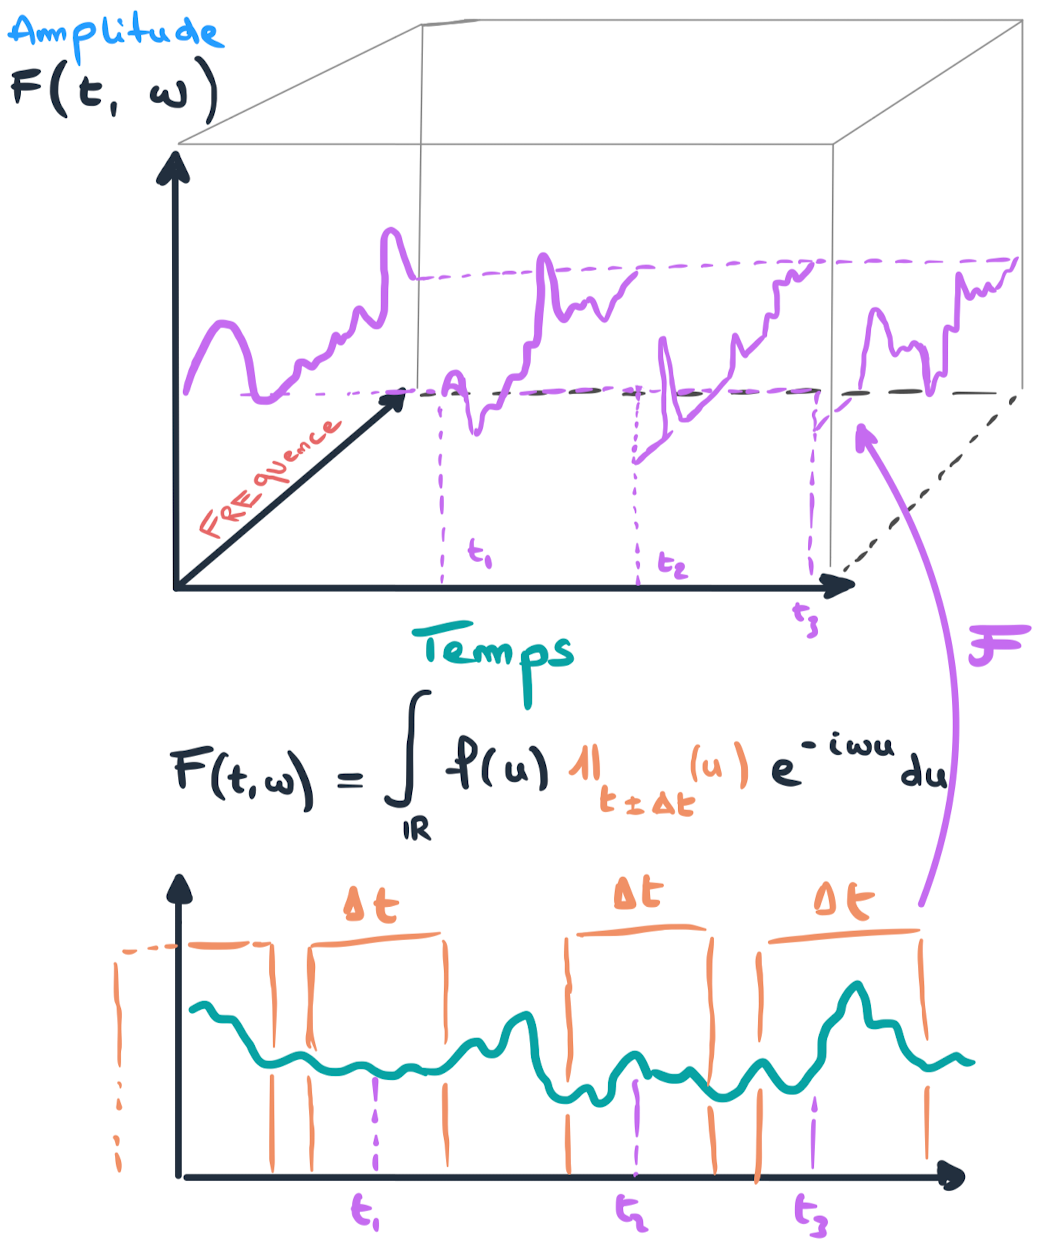
\includegraphics[width=\textwidth]{images/sketches/STFT.png}
        \caption{Transformée de Fourier à court terme d'une fonction}
        \label{fig:STFT}
    \end{figure}
\end{minipage}
\hfill
\begin{minipage}{0.60 \textwidth}
 
    Cependant contrairement à ce que peut suggérer le dessin présenté ici, la résolution fréquentielle n'est pas parfaite. Elle est d'ailleurs dans le cadre de la Transformée de Fourier à court terme constante, que ce soit sur le domaine temporel ou le domaine fréquentiel. La résolution fréquentielle est donc constante quelque soit la fréquence considérée.

    \question{
        \smallskip\centering
        Quel est le problème avec cette approche ?
    }

    le problème ne vient pas du monde mathématique mais plutôt du monde réel : les signaux que l'on observent présentent la caractéristique suivante : Les signaux de basse fréquence ont tendance à s'étendre sur la durée, et les signaux de hautes fréquences ont tendance à être très localisées, sous forme d'impulsion. Il devient alors clair que pour correctement identifier et localiser les fréquences présentes dans un signal, il est judicieux (voire parfois nécessaire) de varier la résolution fréquentielle et temporaire (limitées par le théorème d'indétermination de Heisenberg) en fonction de ce qui est le plus difficile à distinguer. C'est ce que proposent les ondelettes.
    
\end{minipage}

\subsubsection{Théorie de la base ondelettes}

\textbf{Transformée en ondelettes}

Introduisons maintenant de façon plus formelle les ondelettes et regardons leurs propriétés intéressantes dans le cadre du lissage de trajectoires.

on définit la transformée en ondelettes vis à vis de l'ondelette mère $\psi$ d'une fonction $f$ par :

$$F : \begin{array}{ccc}
  \mathds R \times \mathds R_+  &\longrightarrow & \mathds R
    \\
   (t,s) & \longmapsto & \displaystyle\frac 1 { \sqrt{|s|}} \int_{\mathds R} f(\colorize{u}) \psi \left( \frac{\colorize{u}-t}{s} \right) \mathrm d \colorize{u}
\end{array}$$

\brain{on peut remarquer que la formule de la transformée en ondelettes ressemble à une projection : $\displaystyle\frac{\langle f, \psi_{t,s} \rangle_{\mathds L^2}}{|| \psi_{t,s} ||}$. Cela vient en quelque sorte motiver la section suivante}

\textbf{Base d'ondelettes}

$$
\left( \psi_{k,n} : t \mapsto \frac 1 {\sqrt{2^k}} \psi( \frac{t - 2^k n}{2^k} ) \right)_{(k,n) \in \mathds Z^2} \textsf{ est une base } \vcenter{\hbox{$\underset{\| \cdot \|}{\perp}$}} \textsf{ de } \mathds L^2
$$
 
\info{notons que les résolutions sont des puissances de 2, ceci est un détail qui demandera une implémentation particulière dans le cadre des données réelles : il faudra faire attention à ce que le nombre de points que l'on donne dans l'algorithme de transformée rapide en ondelettes soit aussi une puissance de 2.}

\textbf{Propriétés principales des ondelettes}

\smallskip

\begin{itemize}
    \item \textbf{Approximation dans l'espace fréquentiel-temporel} : La transofrmée en ondelettes ( $\mathcal W : f \mapsto \langle f \, | \, \psi_{t,s} \rangle$ ) est une isométrie de $\mathds L^2$. Cela nous permet donc d'affirmer que $|| f - \hat f ||_{\mathds L^2} = || \mathcal W f - \mathcal W \hat f ||_{\mathds L^2}$. Ainsi on peut travailler dans l'espace des ondelettes pour approximer (dans notre cas lisser les trajectoires) des fonctions et contrôler l'approximation directement dans le domaine fréquence-temporel tout en le conservant dans le domaine temporel. \citationrequise
    % @ todo : compléter citation — STFT : talk de Stéphane Mallat

    \item \textbf{Propriété de Fast Decay}
\end{itemize}



\subsubsection{Motivation dans le cadre de l'analyse de données fonctionnelles}

\subsubsection{Effets du lissage à ondelettes sur la régularité locale}



\section{Estimation adaptative}

\subsection{Estimation adaptative de la fonction moyenne}



L'idée du lissage adaptatif est que chaque quantité évaluée en un point $t \in \mathcal T$ tire parti différemment des information du voisinage de $t$. Il semble intuitif que le processus moyen ($\mu = \esperance{X}$) considère des informations d'un voisinage assez large du processus et que celui-ci soit \og assez lisse \fg. Pour déterminer une fenêtre adaptée à l'estimation de la moyenne, on définit une grille de fenêtres à évaluer $\mathfrak H = (h_i)_{1:r}$ que l'on choisit en minimisant un risque spécifiquement adapté :

\begin{equation*}
	\widehat{ h_\mu^* } = \argmin\limits_{h \in \mathfrak H} R_\mu( \, t \, , h \, )
\end{equation*}

\noindent Déterminons maintenant ce risque.

\subsubsection{Méthode Golovkine et al. : indépendance}

Dans le cadre de données indépendantes, on peut invoquer la Loi des Grands Nombres pour approximer l'espérance par la moyenne empirique.
On effectue une suite d'approximations de la façon suivante :

\begin{figure}[H]
	\centering
	\begin{tikzcd}[column sep=6cm, row sep=2cm]
		\widetilde{\mu_{\mathcal W}} \arrow[r, "\textsf{absence points } \mathcal W"] &\widetilde{\mu} \arrow[d, "LGN"]
		\\
		\widehat \mu \arrow[u, "\textsf{biais } \mathds B"] & \mu
	\end{tikzcd}
	\caption{Schéma du découpage du contrôle des erreurs}
\end{figure}

On détermine alors fenêtre de lissage en minimisant le risque suivant \cite{golovkine2021adaptive} :

\begin{equation*}
	R_\mu^{[Golovk.]}(t, h) = \underbracket{q_1^2 h ^{2H_t}}_{\textsf{contrôle du biais}} +
	\underbracket{\frac{q_2^2}{\mathcal N_\mu(t, h)}}_{\textsf{contrôle de la variance}} +
	\underbracket{q_3^2 \bigl[ \frac{1}{\sum_k w_k} - \frac 1 n \bigr]}_{\textsf{pénalise absence de points}}
\end{equation*}

\info{
	Il est tout à fait  possible de regarder directement l'erreur d'approximation entre $\widetilde{\mu_{\mathcal W}}$ et $\mu$. Toutefois, le choix de Golovkine est avant tout un choix pédagogique, pour signaler et renforcer l'idée qu'il faut faire attention à l'erreur d'approximation entre l'inobservable et le véritable processus ( $\mathds E \, X$ vs $\frac 1 N \sum X_i \neq \frac 1 N \sum \widehat X_i$)
}

Afin de prendre en compte la dépendance, que l'on doit contrôler aussi, on raisonne plutôt de la façon suivante.

\subsubsection{Méthode MPV : dépendance}

Lorsque l'on traite le cas de la dépendance, il est tout de suite plus délicat d'obtenir la convergence d'estimateurs de moments d'une loi. MPV utilise ce découpage du risque pour déterminer une fenêtre de lissage adaptée à l'estimation de la fonction moyenne :

\begin{figure}[H]
	\centering
	\begin{tikzcd}[column sep=6cm, row sep=2cm]
		\widetilde{\mu_{\mathcal W}} \arrow[r, "\textsf{absence points } \mathcal W", color=flatuicolors_light_gray] \arrow[dr, "\textsf{MPV : absence points } P_N + \textsf{ dépendance } \mathds D", flatuicolors_green, sloped] &\widetilde{\mu} \arrow[d, "LGN", color=flatuicolors_light_gray]
		\\
		\widehat \mu \arrow[u, "\textsf{biais } \mathds B"] & \mu
	\end{tikzcd}
	\caption{Schéma du découpage du contrôle des erreurs}
\end{figure}

On détermine cette fois-ci la fenêtre de lissage en minimisant le risque suivant \cite{maissoro-SmoothnessFTSweakDep} :

\begin{equation*}
	R_\mu( \, t \, , h \, ) =
	\underbracket{L_t^2 h ^{2H_t} \mathds B( \, t, h, 2H_t \,) }_{\textsf{contrôle du biais}}
	+ \underbracket{\sigma^2 \mathds V_\mu( \, t, h \, ) }_{\textsf{contrôle de la variance}}
	+ \underbracket{\frac{\mathds D_\mu( \, t \, )}{P_N(t, h)}}_{\textsf{contrôle de la dépendance}}
\end{equation*}






\subsection{Estimation adaptative de l'opérateur de covariance}

On souhaite désormais estimer la quantité la covariance de la loi de notre processus. Si il semblerait naturel d'évaluer :

\begin{equation*}
	C_X(s,t) = \esperance{ \bigl(X(t) - \mu(t)\bigr) \cdot \bigl( X(s) - \mu(s) \bigr) }
\end{equation*}

la quantité qui nous intéresse, in-fine est l'opérateur de covariance :

\begin{equation*}
	c[ \, f \,] = \int_I f(u)c(u, \, \cdot \, ) \, du
\end{equation*}

C'est parceque c'est cet opérateur qui nous donnera, notamment, les vecteurs et valeurs propres de la décomposition dans la base FPCA, aussi connue sous le nom de décomposition de Karhunen-Loève.

\bigskip

On comprend bien que la covariance est une quantité qui mesure la dispersion des données et qu'il est donc naturel de s'intéresser beaucoup plus aux fines variations dans un voisinage proche du couple $(t,s)$ des différents temps qui nous intéressent. Cela vient motiver, une fois de plus l'intérêt de l'utilisation d'un lissage adaptatif qui nous est donné par la minimisation du risque suivant ~\cite{maissoro-SmoothnessFTSweakDep} :

\begin{equation*}
	R_\Gamma( t, h ) =
\end{equation*}

\subsection{Estimation adaptative de l'auto-covariance des séries temporelles fonctionnelles}

\input{content/chapter_2/estimation_adaptative__autocovariance.tex}
\chapter{Détermination du diamètre optimal des intervalles à considérer pour l'estimation de la régularité locale }
\minitoc%

\section{Introduction et Objectifs de la simulation}

\section{Simulation de données $\operatorname{FAR}(1)$ Localement Hölderiennes}

La fonction $H : t \mapsto H_t$ qui a été choisie est la suivante :

$$
H^{[0.4, 0.8, 5, 0.5]}_{\textsf{logistic}} : \begin{array}{ccc}
    [0,1] & \longrightarrow & [0.4, 0.8]
    \\
    t & \longmapsto & 0.4 + \frac{(0.8 - 0.4)}{1 + e^{-5(t - 0.5)}}
\end{array}
$$

\begin{figure}[H]
    \centering
    \begin{tikzpicture}
        \begin{axis}[
            xlabel=$t$,
            ylabel={$H^{[0.4, 0.8, 5, 0.5]}_{\textsf{logistic}}(t)$},
            xmin=0, xmax=1,
            ymin=0.4, ymax=0.8,
            axis lines=center,
            axis on top=true,
            domain=0:1,
            samples=100,
            ]
            \addplot [mark=none,smooth,blue] {0.4 + (0.8 - 0.4)/(1 + exp(-5*(x - 0.5)))};
            \addplot [only marks,mark=*] coordinates {
        (0.3,0.51)
        (0.4,0.55)
        (0.5,0.6)
        (0.6,0.65)
        (0.7,0.69)
        (0.8,0.73)
    };
        \end{axis}
        \end{tikzpicture}
    \caption{Hurst Function : Logistic}
    \label{plot:hurst-logistic}
\end{figure}

$$\forall t \quad L_t = 1$$

$$
\mu : \begin{array}{ccc}
    [0,1] & \longrightarrow & \mathbb R
    \\
    t & \longmapsto & 4 \cdot \sin\bigl( \frac 3 2 \pi \cdot t \bigr)
\end{array}
$$
    
\begin{figure}[H]
    \centering
    \begin{tikzpicture}
        \begin{axis}[
            xlabel=$t$,
            ylabel=$\mu(t)$,
            xmin=0, xmax=1,
            ymin=-4, ymax=4,
            axis lines=center,
            axis on top=true,
            domain=0:1,
            samples=100,
            ]
            \addplot [mark=none,smooth,blue] {4*sin(deg(3/2*pi*x))};
        \end{axis}
        \end{tikzpicture}
    \caption{Mean function : $\mu(t) = 4 \cdot \sin\bigl( \frac 3 2 \pi \cdot t \bigr)$}
    \label{plot:mu}
\end{figure}


$$
\vec t = \begin{bmatrix} 0.3 \\ 0.4 \\ 0.5 \\ 0.6 \\ 0.7 \\ 0.8 \end{bmatrix}
\quad\quad
H(\, \vec t \,) = 
\begin{bmatrix}
    0.51 \\ 0.55 \\ 0.6 \\ 0.65 \\ 0.69 \\ 0.73
\end{bmatrix}
$$

$$
\beta : \, \begin{array}{ccc}
    [0,1]^2 & \longrightarrow & \mathbb R
    \\
    (t,s) & \longmapsto & \frac 9 4 t\sqrt{ s(1-s) }
\end{array}
$$

\begin{tikzpicture}
    \begin{axis}[
        xlabel=$t$,
        ylabel=$s$,
        zlabel=$\beta(t,s)$,
        xmin=0, xmax=1,
        ymin=0, ymax=1,
        zmin=0, zmax=1,
        axis lines=center,
        axis on top=true,
        domain=0:1,
        samples=50,
        ]
        \addplot3 [surf] {9/4*x*sqrt(y*(1-y))};
    \end{axis}
\end{tikzpicture}

$$
\varphi : \begin{array}{ccc}
    [0,1] & \longrightarrow & \mathbb R
    \\
    t & \longmapsto & \int_{[0,1]} f(u) \beta(t,u) \, du
\end{array}
$$

$$
\vec N = [ 100, 200, 300, 400]
$$

$$
\vec \Delta = [ 0.01 \cdots (0.01 + k\cdot0.01)\cdots 0.2 ]_{k \in 0:30}
$$

En résumé :

\begin{table}[H]
    \centering
    \begin{tabular}{l|l|ll|l|}
    \cline{2-5}
    \textbf{}                                                         & \textbf{nombre de valeurs testées} & \multicolumn{1}{l|}{\textbf{de}} & \textbf{jusqu'à}         & \textbf{valeur}          \\ \hline
    \multicolumn{1}{|l|}{\textit{\textbf{$\Delta$}}}                  & $30$                               & $0.01$                        & $0.2$                   & \cellcolor[HTML]{C0C0C0} \\
    \multicolumn{1}{|l|}{\textit{\textbf{$\lambda$}}}                 & $30$                               & $30$                             & $480$                    & \cellcolor[HTML]{C0C0C0} \\
    \multicolumn{1}{|l|}{\textit{\textbf{$N$}}}                       & $4$                                & $100$                            & $400$                    & \cellcolor[HTML]{C0C0C0} \\
    \multicolumn{1}{|l|}{\textit{\textbf{fonction de Hurst ($H_t$)}}} & $2$                                & logistique                       & escalier                 & \cellcolor[HTML]{C0C0C0} \\
    \multicolumn{1}{|l|}{\textit{\textbf{nb simulations MC}}}         & \cellcolor[HTML]{C0C0C0}           & \cellcolor[HTML]{C0C0C0}         & \cellcolor[HTML]{C0C0C0} & $200$                    \\ \hline
    \end{tabular}
    \caption{Hyper-paramètres de la simulation Monte-Carlo}
    \label{tab:hyperparam-mc}
    \end{table}


\section{Prélissage des données simulées}




\section{Qualité de l'estimation des incréments quadratiques moyens}

\newcommand{\thetaA}{\Theta_{1 \rightarrow \overset{3}{\underset {2}{}}}}
\newcommand{\cindexA}{_{1 \rightarrow \overset{3}{\underset {2}{}}}}
\newcommand{\thetaB}{\Theta_{\overset 1{\underset{2}{ }} \rightarrow3}}
\newcommand{\cindexB}{_{\overset 1{\underset{2}{ }} \rightarrow3}}
\newcommand{\thetaC}{\Theta_{1 \rightarrow 2 \rightarrow 3}}
\newcommand{\cindexC}{_{1 \rightarrow 2 \rightarrow 3}}
\newcommand{\notequiv}{\overset {\textsf{\faTimes}} \iff}
\newcommand{\yesequiv}{\overset {\textsf{\faCheck}} \iff}

Il y a différentes manières de définir les paramètres de régularité $\hat H_t$ et $\hat L_t$. En effet il est possible de définir $\hat H_t$ en utilisant $\hat \theta (t_1, t_2)$ mais aussi en utilisant $\hat \theta (t_2, t_3)$ ($\theta(t_1, t_3)$ est forcément utilisé\footnote{$\hat H_t$ ne serait même pas bien défini pour le couple $\theta(t_1, t_2)$, $\theta(t_2, t_3)$}). De même pour $\hat L_t$. On peut donc se demander quels sont les meilleurs $\theta(u,v)$ avec $u,v \in \{t_1, t_2, t_3\}$ à utiliser pour obtenir la meilleure estimation de $H_t$ et $L_t$ ainsi que leur $\Delta$ optimal associé pour l'estimation de ces paramètres.

Le problème est que le proxy $\theta$ est défini comme une espérance, et donc n'est pas observable. On ne peut donc pas directement comparer $\hat \theta(u,v) = \sum_i|\widehat X_i(u) - \widehat X_i(v)|^2$ et $\theta(u,v) = \esperanceloi X { |X(u) - X(v)|^2 }$, à moins d'avoir fait le calcul de l'expression explicite en connaissant la loi du processus initial. 

On peut cependant comparer $\hat \theta(u,v)$ et $\widetilde \theta(u,v) = \frac 1 N \sum_i |X_i(u) - X_i(v)|^2$ qui est un estimateur de $\theta(u,v)$, et que l'on obtient aisément avec la simulation. On peut ainsi déterminer pour quelle valeur de $\Delta$ et quel couple $(u,v)$ on dispose de la meilleur estimation du $\tilde \theta$, qui est entre-autre le meilleur estimateur que l'on pourrait espérer de $\theta$.


Le meilleur couple (au sens donné dans cette section) est pris comme étant les deux $\hat \theta(u,v)$ réalisant les risques minimaux par rapport au $\tilde \theta$ sur les 3 couples $(u,v)$ possibles. 

    \begin{table}[H]
        \centering
        \begin{tabular}{l|ll|}
            \cline{2-3}
            & $\lambda < 120$                                                                                            & $\lambda \geq 120$                                                                 \\ \hline
            \multicolumn{1}{|l|}{$H_t < 0.6$}    & \multicolumn{1}{l|}{\begin{tabular}[c]{@{}l@{}}$\thetaC$\\ \\ \\ $\Delta^- \rightarrow 0.01$\end{tabular}} & \begin{tabular}[c]{@{}l@{}}$\thetaA$\\ \\ $\Delta^+ \rightarrow 0.2$\end{tabular}  \\ \cline{2-3} 
            \multicolumn{1}{|l|}{$H_t \geq 0.6$} & \multicolumn{1}{l|}{\begin{tabular}[c]{@{}l@{}}$\thetaA$\\ \\ $\Delta^- \rightarrow 0.2$\end{tabular}}     & \begin{tabular}[c]{@{}l@{}}$\thetaC$\\ \\ $\Delta^+ \rightarrow 0.01$\end{tabular} \\ \hline
        \end{tabular}
        \caption{Tableau récapitulatif des $\Theta$ optimaux : Risque individuel sur $\tilde \theta(u,v)$}
        \label{tab:recap_theta_single}
    \end{table}



\section{Qualité de l'estimation de la régularité locale}

Les simulations de Monte Carlo permettent d'avoir accès directement à la véritable régularité de la courbe en chaque point. Nous allons dans l'étude du comportement du $\Delta$ essayer de tirer profit de cet avantage que ne possède pas le praticien qui utilise des données réelles.


\begin{table}[H]
    \centering
    \begin{tabular}{l|ll|}
    \cline{2-3}
                                          & $\lambda < 120$                                                                                                                                                                                                                                                                                    & $\lambda \geq 120$                                                                                                                                                                         \\ \hline
    \multicolumn{1}{|l|}{$H_t \leq 0.65$} & \multicolumn{1}{l|}{\begin{tabular}[c]{@{}l@{}}$\yesequiv \mathcal R$\\ $\yesequiv \Delta^*$\\ $\Delta^- \downarrow 0.01$\end{tabular}}                                                                                                                                             & \begin{tabular}[c]{@{}l@{}}$\simeq \yesequiv \mathcal R$\\ $\notequiv \Delta^*$\\ $\Delta^+ \rightarrow [\leq 0.6] 0.1/0.2 [\geq 0.6]$\end{tabular}                            \\ \cline{2-3} 
    \multicolumn{1}{|l|}{$H_t > 0.65$}    & \multicolumn{1}{l|}{\begin{tabular}[c]{@{}l@{}}$\yesequiv \mathcal R$\\ $\notequiv \Delta^*$\\ \faExclamationTriangle $H=0.7 : \Delta^- = 0.02$\\ \faExclamationTriangle $H = 0.73 : \Delta^- = 0.2$\end{tabular}} & \begin{tabular}[c]{@{}l@{}}$\thetaA$\\ \faExclamationTriangle $H=0.7 : \Delta^+ = 0.02$\\ \faExclamationTriangle $H = 0.73 : \Delta^+ = 0.2$\end{tabular} \\ \hline
    \end{tabular}
    \caption{Tableau récapitulatif des $\Delta$ optimaux : Risque sur $H_t$}
    \label{tab:recap_delta_H}
    \end{table}

\section{Qualité de l'estimation des couples d'incréments utilisés dans l'estimation de la régularité}


\info{
    on rappelle les notations suivantes :

    \begin{itemize}
        \item vrai : $\theta = \mathds E \bigl[ \, f(X) \, \bigr]$
        \item intangible : $\widetilde \theta = \frac 1 N \sum_i f(X_i)$
        \item observable : $\hat \theta = \frac 1 N \sum_i f(\widehat X_i)$ 
    \end{itemize}
}

L'estimateur du paramètre de régularité $H_t$ est donné par :

$$\hat H_t = \frac{ \log \hat \theta(t_1, t_3) - \log \hat \theta(t_1, t_2) }{2 \log 2}$$

ou bien encore :

$$\hat H_t = \frac{ \log \hat \theta(t_1, t_3) - \log \hat \theta(t_2, t_3) }{2 \log 2}$$


autrement dit :

en posant $\thetaA = \begin{bmatrix} \theta(t_1, t_3) \\ \theta(t_1, t_2) \end{bmatrix}$ et $\thetaB = \begin{bmatrix} \theta(t_1, t_3) \\ \theta(t_2, t_3) \end{bmatrix}$

$$
\hat H_t : \Theta \longmapsto \frac{ \log \Theta_1 - \log \Theta_2 }{2 \log 2}
$$

C'est pourquoi, étant donné que le meilleur estimateur que l'on puisse espérer soit $\bigl(\hat H_t( \tilde \thetaA)$ ou $\hat H_t( \tilde \thetaB)\bigr)$, on va s'intéresser désormais à l'estimation conjointe des deux $\theta(u,v)$ utilisés dans l'estimation de $H_t$ comme critère de sélection du diamètre $\Delta$.

\begin{figure}[H]
    \centering
    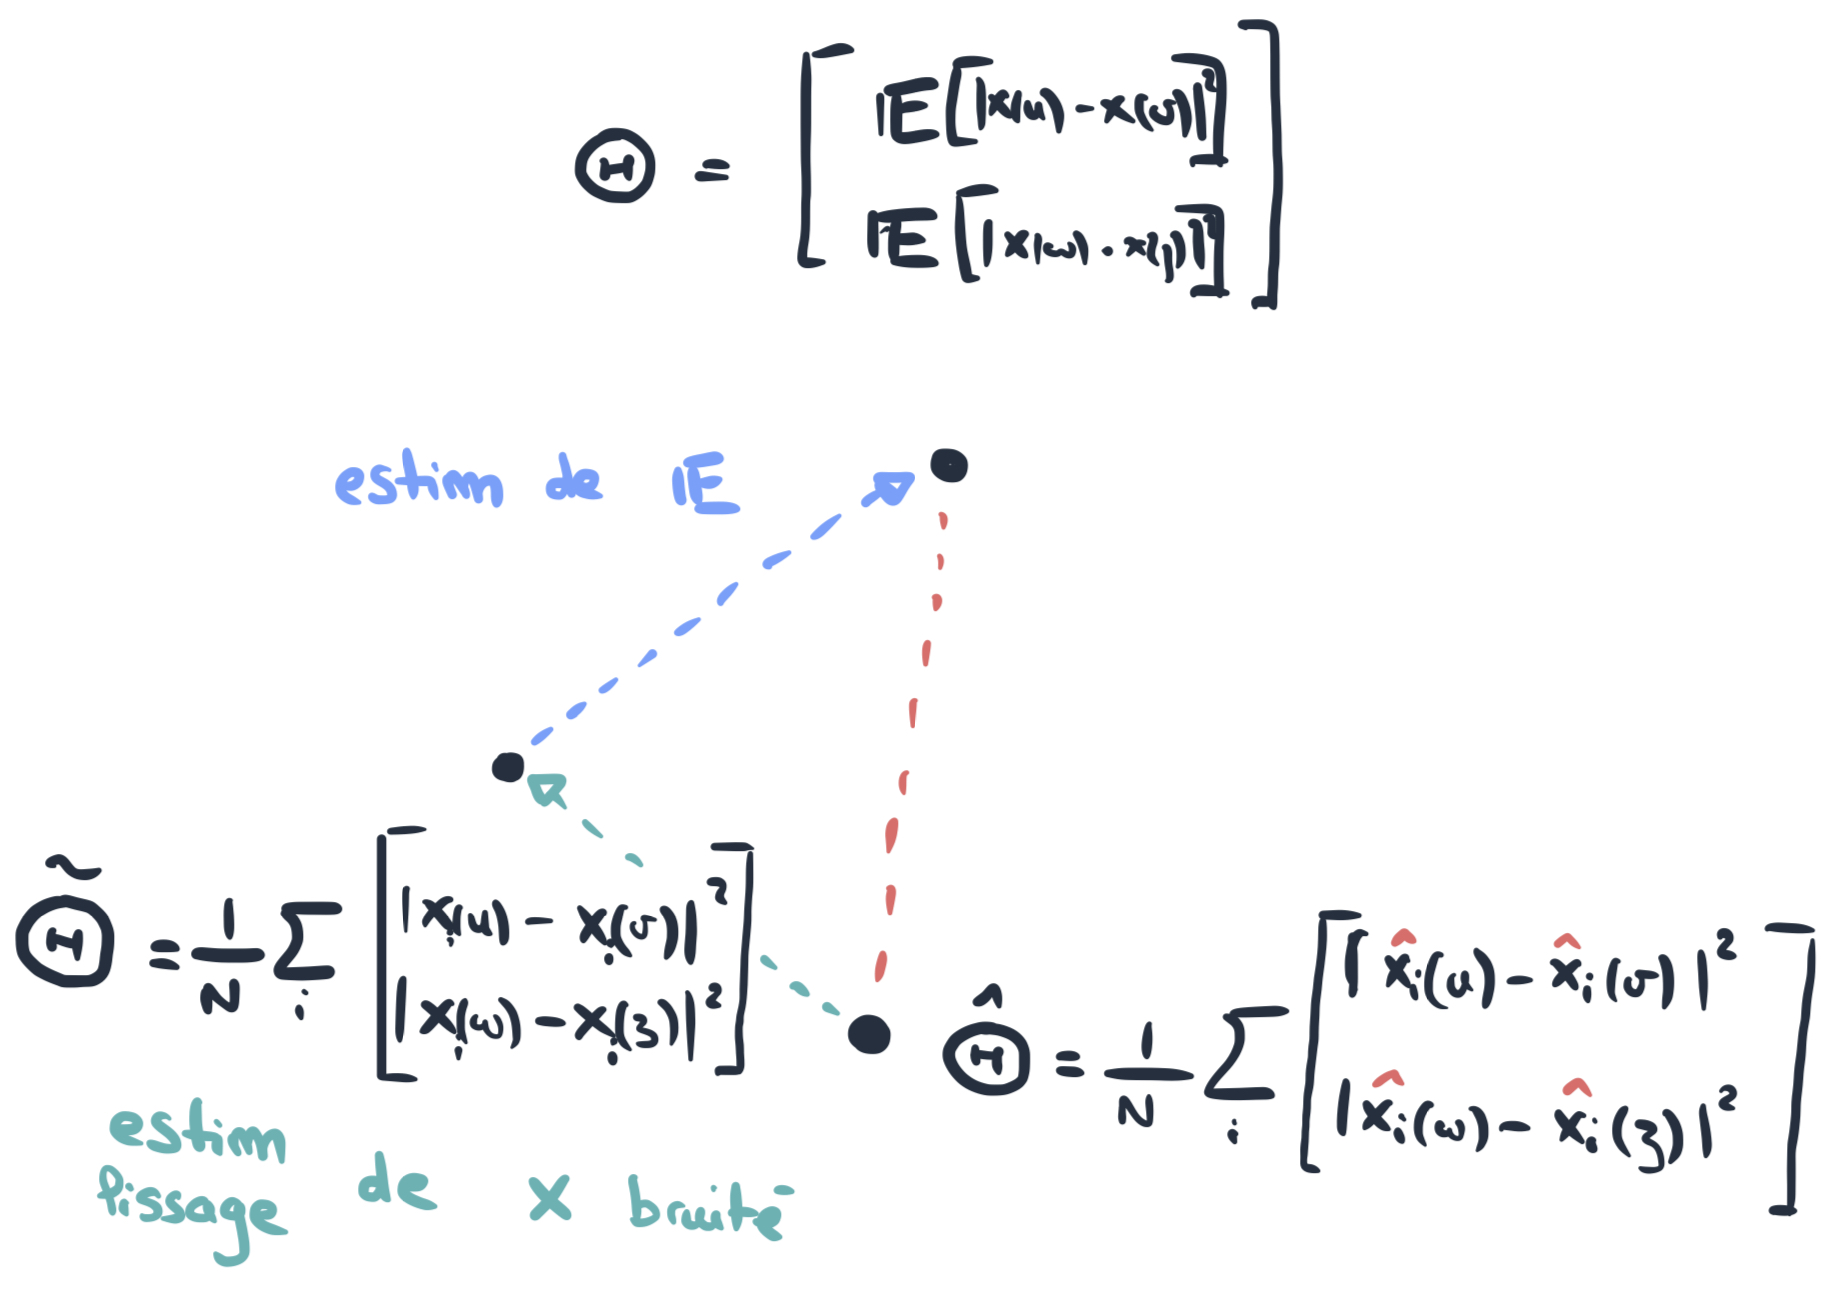
\includegraphics[width=0.7\textwidth]{Images/sketches/theta_biais.jpg}
    \caption{title}
    \label{fig:sketch_theta_biais}
\end{figure}


Pour cela on considère la distance euclidienne usuelle pour des vecteurs de $\R 2$

$$R(\Theta, \Delta) = \distnorme 2 {\widehat \Theta(\Delta)} {\widetilde \Theta(\Delta)}$$

et on nomme $R\cindexA = R( \thetaA , \, \cdot \, )$ et $R\cindexB = R( \thetaB, \, \cdot \, )$

\begin{table}[H]
    \centering
    \begin{tabular}{l|ll|}
    \cline{2-3}
                                         & $\lambda < 120$                                                                                                                                                                                                                                     & $\lambda \geq 120$                                                                             \\ \hline
    \multicolumn{1}{|l|}{$H_t < 0.6$}    & \multicolumn{1}{l|}{\begin{tabular}[c]{@{}l@{}}$\yesequiv \mathcal R, \Delta^*$\\ $\Delta^*_- = 0.01$\end{tabular}}                                                                                                                                 & \begin{tabular}[c]{@{}l@{}}$\thetaB$\\ $\Delta^*_+ = 0.2$\end{tabular}                         \\ \cline{2-3} 
    \multicolumn{1}{|l|}{$H_t \geq 0.6$} & \multicolumn{1}{l|}{\begin{tabular}[c]{@{}l@{}}$\thetaB$\\ $\Delta^*_- = 0.2$\\ \\\faExclamationTriangle $H=0.7 : \Delta^- = 0.01 \oplus \yeqequiv \mathcal R$\\ \\\faExclamationTriangle $H=0.8 : \thetaA$\end{tabular}} & \begin{tabular}[c]{@{}l@{}}$\yesequiv \mathcal R, \Delta^*$\\ $\Delta^*_+ = 0.01$\end{tabular} \\ \hline
    \end{tabular}
    \label{tab:recap_delta_eucl}
    \caption{Tableau récapitulatif des $\Delta$ optimaux : Risque euclidien sur $\tilde \Theta$}
    \end{table}

\section{Détermination d'un critère de choix du diamètre $\Delta$ des intervalles à considérer pour l'estimation de la régularité locale}


Maintenant que l'on a déterminé que l'on souhaite travailler sur un les couples $\thetaB = \begin{bmatrix} \theta(t_1, t_3) \\ \theta(t_2, t_3) \end{bmatrix}$ et $\thetaA = \begin{bmatrix} \theta(t_1, t_3) \\ \theta(t_1, t_2) \end{bmatrix}$, il nous faut déterminer un critère pour déterminer quel couple est plus judicieux pour la méilleure estimation en pratique des paramètres de régularité locale.

L'heuristique est la suivante : dans nos simulations, on a le luxe de pouvoir faire 200 simulations de monte carlo et obtenir le $\Delta^*$ le plus proche du $\Delta$ optimal pour estimer la régularité. Dans la pratique, obtenir un tel $\Delta$ optimal n'est pas réaliste, on se trouvera soit un peu en dessous, soit un peu au dessus. L'idée est donc de favoriser le couple de $\theta(u,v)$ qui possède le plus grand plateau autour du $\Delta^*$ pour le risque quadratique \emph{si l'écart de risque quadratique entre les deux couples n'est pas trop important}. Si l'un est beaucoup plus performant que l'autre, on choisira le plus performant. Mais si la performance des deux est à peu près équivalente, autant sélectionner celui qui dans la pratique (sans avoir 200 réplications indépendantes) nous donnera le plus de flexibilité sur l'erreur commise en sélectionnant un $\Delta$ autour du $\Delta^*$ dû à la fluctuation statistique.

\subsection{Détermination d'un seuil pour l'équivalence de risque quadratique}

Il nous faut maintenant déterminer ce que l'on considère comme étant deux risques "équivalents". Pour cela on va déterminer pour différentes valeurs du véritable $H$ le seuil $\varepsilon$ sur le risque tel que $R\cindexA(\Delta + \delta) + \varepsilon$ induit une erreur d'au maximum $10$\% sur le H estimé. On viendra ensuite déterminer les $\delta$ qui en moyenne correspondent à ce seuil $\varepsilon$ pour les différentes valeurs de $H$.

\subsection{Détermination du meilleur couple à risque \og équivalent \fg}

\subsubsection{en utilisant les pentes}


Une méthode possible serait de définir la pente à gauche et la pente à droite de la façon suivante : 

$$a_g : \Delta, \delta \mapsto \frac{R(\Delta) - R(\Delta - \delta)}{\delta}$$
$$a_d : \Delta, \delta \mapsto \frac{R(\Delta + \delta) - R(\Delta)}{\delta}$$

On peut définir les pénalisations suivantes pour déterminer le meilleur couple à risque équivalent en terme de plateau, en pénalisant les larges différence entre la pente à gauche et à droite :

$$m_q(\Delta, \delta) = \frac{a_g^2(\Delta, \delta) + a_d^2(\Delta, \delta)}{2}$$


\subsubsection{en utilisant les valeurs de risque}
une autre méthode est de regarder :

$$R_2(\Delta^*_2) \geq R_1(\Delta^*_1)$$

$$dR = \bigl\vert R_1(\Delta^*_1) - R_2(\Delta^*_2) \bigr\vert$$

on compare désormais les valeurs de :

$$r_g^{[2]} = R_2(\Delta^*_2 - \delta) - dR$$ 
$$r_d^{[2]} = R_2(\Delta^*_2 + \delta) - dR$$ 

aux valeurs

$$r_g^{[1]} = R_1(\Delta^*_1 - \delta)$$ 
$$r_d^{[1]} = R_1(\Delta^*_1 + \delta)$$

avec le critère de sélection suivant :

$$\argmin \bigl( \frac{r_g^{[1]} + r_d^{[1]}}{2}, \frac{r_g^{[2]} + r_d^{[2]}}{2}  \bigr)$$

Pour pénaliser les solutions où la pente à gauche est très différente de la pente à droite en magnitude, on peut considérer d'élever $r_g$ et $r_d$ au carré.

$$\argmin \bigl( \frac{(r_g^{[1]})^2 + (r_d^{[1]})^2}{2}, \frac{(r_g^{[2]})^2 + (r_d^{[2]})^2}{2}  \bigr)$$

\subsubsection{résultat}
\chapter{Note et réflexions personnelles sur le stage}

\section{Implémentation d'un package R}

\section{Apprentissage}

\section{Communication}

\appendix
\pagenumbering{roman}
\chapter{Détails techniques et théoriques}

\section{Données fonctionnelles : formellement}
\label{annexe:fda-formel}
\subsubsection{Définition formelle}

Pour éviter d'alourdir les notations, on se place dans le cas où les fonctions sont à valeurs dans $\mathds R$ et à support sur un intervalle fermé $I$ de $\mathds R$. Toutefois, on peut très bien considérer des fonctions à valeurs dans $\mathds R^d$ et à support sur un compact $K$ de $\mathds R^p$ sans perte de généralités.

\begin{definition}[données fonctionnelles ]

    On appelle données fonctionnelles, un échantillon $\famfinie x 1 n$ de fonctions continues $x_i : I \rightarrow \R d$ issues d'un processus $X$ défini comme ci-dessous :

    $$X :
        \begin{array}{ccc}
            \Omega & \longrightarrow & \mathcal C(I, \mathds R)
            \\
            \omega & \longmapsto     & X(\omega) = x
        \end{array}
    $$

\end{definition}

\subsubsection{Résultats importants}

On énonce désormais le théorème central de l'analyse de données fonctionnelles qui n'est autre que la décomposition dans la base FPCA de notre processus.

\begin{rem}
	on notera que dans le cadre des données fonctionnelles, on ne travaille pas de façon générale avec la covariance :

	$$C_X : (s,t) \mapsto \esperance{ \left[X - \mu\right](s) \cdot \left[X - \mu\right](t) }$$

	On travaille plutôt avec l'\textbf{opérateur} de covariance :

	\begin{equation*}
		c : \begin{array}{ccc}
			\mathds L^2 & \longrightarrow & \mathds L^2                             \\
			f           & \longmapsto     & \int\limits_I f(u)C_X(u, \cdot \,) \,du
		\end{array}
	\end{equation*}

	C'est parceque cet opérateur est linéaire continu (car Hilbert-Schmidt donc borné pour la norme d'opérateur) symétrique semi-défini positif (pour le produit scalaire de $\mathds L^2$) et que l'on peut donc en faire une décomposition spectrale sur une base orthonormale de vecteurs propres associés à des valeurs propres positives. Cette décomposition est à la base des approximations que le praticien effectuera ainsi qu'à la base de la dérivation de nombreux théorèmes et propriétés.
\end{rem}

\bigskip

Etant donné que l'on traîte des données fonctionnelles, on considère la géométrie usuelle de $\mathds L^2(\mathds R, \, \lambda)$ et on note ainsi

\begin{equation*}
	\prodscalselon \cdot \cdot {\mathds L^2}: \begin{array}{ccc}
		\mathds L^2 \times \mathds L^2 & \longrightarrow & \mathds R
		\\
		(f,g)                          & \longmapsto     & \int f(u)g(u) \, d\lambda(u)
	\end{array}
\end{equation*}


le produit scalaire que l'on considère pour manipuler les données fonctionnelles.


% https://stackoverflow.com/a/4008463 : no page break
\begin{minipage}{\textwidth}
	\begin{thm}[Karhunen-Loeve]
		\emph{référence :} ~\cite[pages : 238-239-241]{kokoszka2017introduction}

		\textbf{Hypothèses :}

		\begin{equation*}
			\boxed{
				\begin{array}{ll}
					\textsf{\faCaretSquareRight} & X \in \mathds L^2( \Omega, \mathcal C(I, \mathds R))
					\\ \\
					\textsf{\faCaretSquareRight} & \textsf{covariance : } C : \begin{array}{ccc}
						                                                          \mathds L^2( \Omega, \mathcal C(I, \mathds R)) & \longrightarrow & \mathcal C(I^2, \mathds R)
						                                                          \\
						                                                          X                                              & \longmapsto     & C_X
					                                                          \end{array}
					\\ \\
					                             & \textsf{ie : } C_X : (s, t) \mapsto C_X(s,t) \textsf{ est continue}
					\\ \\
					\textbf{\faIcon{asterisk}}   & \textsf{opérateur covariance} \, c_X[ \, \cdot \, ] : \begin{array}{ccc}
						                                                                                     \mathcal C(I, \mathds R) & \longrightarrow & \mathcal C(I, \mathds R)
						                                                                                     \\
						                                                                                     f                        & \longmapsto     & \int_I f(s) C_X(s, \cdot \, ) \, ds\end{array}
					\\\\
					\textsf{\faCaretSquareRight} & \textsf{valeurs propres ordonnées : } \forall p \geq 1, \lambda_{p+1} \leq \lambda_p \quad\quad \lambda_p, \lambda_{p+1} \in \operatorname{sp}(c_X)
					\\ \\
					\textbf{\faIcon{asterisk}}   & \textsf{on pose } \overrightarrow{sp}_{\orthonormal}^{[1,p]}(c_X) \isdef \left\{ \phi_k \in \overrightarrow{sp}_{\orthonormal}( \, c_X \, ) \textsf{ associé à }  \lambda_k, k \in \intervaleint 1 p \, \right\}
				\end{array}
			}
		\end{equation*}

		\textbf{alors :}
		\begin{equation*}
			\boxed{
				\begin{array}{cc}
					\textsf{\faCaretSquareRight} &

					\forall p \geq 1
					\quad
					\argmin\limits_{u_k \in \mathcal C(I, \mathds R)} \mathds E \left\Vert X - \sum\limits_{k=1}^p \prodscalselon {X - \mu} {u_k} {\mathds L^2} u_k \right\Vert^2 = \overrightarrow{sp}_{\orthonormal}^{[1,p]}( \, c_X \, )

					\\
					\\
					\textsf{\faCaretSquareRight} & X = \mu + \sum\limits_{k=1}^{+\infty} \prodscal {X - \mu} {\phi_k} \phi_k
					\\
					                             &
					\\
					                             & \textsf{avec } \phi_k \in \overrightarrow{sp}_{\orthonormal}( \, c_X \, )
				\end{array}
			}
		\end{equation*}

		\label{thm:KL}
	\end{thm}
\end{minipage}
\begin{proof}[\faCogs \, preuve informelle]
	La covariance est un opérateur bilinéaire symétrique défini positif, on peut donc appliquer le théorème de Mercer (équivalent du théorème spectral) qui nous donne une base orthonormale de $\mathds L^2$ sur laquelle on va décomposer notre processus \textbf{centré}.
\end{proof}


\begin{rem}
	pour pouvoir ordonner les valeurs propres dans l'ordre décroissant, et sélectionner les composantes principales les plus informatives, il faut pouvoir réarranger l'ordre de la somme. Pour cela il faut que les valeurs propres forment une famille sommable, une condition suffisante et souvent utilisée est que $\mathds E \Vert X \Vert^2 < \infty$
\end{rem}

\begin{rem}
	la propriété de la section précédente sur l'aspect économe de la base FPCA découle directement de l'assertion
	\begin{equation*}
		\forall p \geq 1
		\quad
		\argmin\limits_{u_k \in \mathcal C(I, \mathds R)} \mathds E \left\Vert X - \sum\limits_{k=1}^p \prodscal {X - \mu} {u_k} u_k \right\Vert^2 = \overrightarrow{sp}_{\orthonormal}^{[1,p]}( \, c_X \, )
	\end{equation*}
	dans le théorème de Karhunen-Loeve.
\end{rem}




\section{Régularité Locale}
\label{annexe:regularite-locale}
Nous avons mentionné que les processus auxquels on allait s'intéresser étaient les processus localement Höldériens de paramètres $\bigl(\alpha(t), L_\alpha(t)\bigr)$. Ce n'est pas tout à fait vrai. Si le coeur de ce que l'on considère sont bel et bien les processus Höldériens, on élargit encore plus la classe des processus que l'on considère en considérant les processus qui sont \textbf{presque} Höldériens.

\question{Qu'est ce qu'on entend exactement par presque Höldérien ?}

pour $u$ et $v$ dans un voisinage de $t$ de dimaètre $\Delta$ :


Ce que l'on demandait pour un processus $X$ est que pour tout $u,v$ dans un voisinage de $t$ de diamètre $\Delta$, il existe  $L_t$ et $H_t$ telle qu'on ait :

\begin{equation*}
	\theta(u,v) \isdef \esperance{ \bigl\vert \, X(u) - X(v) \, \bigr\vert^2 } \leq L_t^2 \, \vert u - v \vert^{2 H_t}
\end{equation*}

on peut alors retrouver la régularité du processus comme un processus Höldérien de paramètres $\bigl(H_t, L_t\bigr)$ d'après le théorème de \nameref{thm:kolmogorov_continuite}.

en réalité il suffit que $\theta(u,v)$ soit suffisamment proche d'un processus localement Höldérien de paramètres $\bigl(H_t, L_t\bigr)$ et que l'on puisse contrôler l'écart entre les deux. Cet écart dépend de $\Delta$ et de la régularité. C'est ce qu'affirme les deux hypothèses suivantes qui sont en fait les hypothèses de régularité qui sont considérées par MPV\cite{maissoro-SmoothnessFTSweakDep}.

\begin{equation*}
	\bigl\vert \theta(u,v)-L_{t}^{2}|u-v|^{2H_{0}}\bigr\vert\leq S_{t}^{2}|u-v|^{2H_{0}}\Delta^{2\beta_{0}}
\end{equation*}

\cite[H6]{maissoro-SmoothnessFTSweakDep}

\begin{equation*}
	\left|\nu_{2}\left(\nabla^{\delta}X(u)-\nabla^{\delta}X(v)\right)^{2}-L_{\delta,t}^{2}|u-v|^{2H_\delta}\right|\leq S_{\delta,t}^{2}|u-v|^{2H_\delta}\Delta^{2\beta_{\delta}}
\end{equation*}


\cite[D1-7]{maissoro-SmoothnessFTSweakDep}


On remarquera que si le processus est localement Höldérien, alors on a un contrôle optimal de l'écart entre $\theta(u,v)$ et $L_t^2 \, \vert u - v \vert^{2 H_t}$.

L'auteur saura donc reconnaître, que bien que ce qui ait été exposé ne soit pas la forme exacte, cela ne change rien à l'idée générale. De plus, cela alourdirait considérablement la rédaction et rendrait la compréhension bien plus difficile de l'objectif du stage.

\pagebreak


\section{Dépendance Faible et LGN version faible}
\label{annexe:weak_dep}

Il y a dans un premier temps ce qu'on appelle la dépendance \og forte \fg, comme la dépendance dite de \og $\alpha$-mixing \fg comme définie dans ~\cite{estimation-dependent-strong-mixing} :


\begin{definition*}[$\alpha-$mixing]

    une suite $X = \suite X i$ de variables aléatoire est dite $\alpha$-mixing si pour tout $n \in \mathds N$


    $$
        \alpha(n) \tend n \infty 0
    $$

    avec : $\alpha(n) = \sup\limits_k \bigl\{ \lvert \proba{A \cap B} - \proba{A}\proba{B} \rvert \quad | \quad A \in \sigma( X_{1:k} ), \, B \in \sigma(X_{k+n : \infty}) \bigr\}$

    en d'autres termes, la \og dépendance \fg \colorize[flatuicolors_blue_devil]{$(\lvert\, \proba{A \cap B} - \proba{A}\proba{B} \,\rvert)$} entre les variables aléatoires $X_k$ et $X_{k+n}$ tend vers 0 lorsque $n$ tend vers l'infini.
\end{definition*}

Ce point de vue est \og fort \fg dans le sens où l'on manipule directement les tribus, et que l'on regarde leur degré d'indépendance via la mesure de probabilité. Il ne s'agit pas de l'approche considérée par MPV qui est plus faible, en se reposant non pas sur l'indépendance des tribus engendrées par la série temporelle mais en exploitant la qualité d'approximation de la série temporelle que l'on étudie par un autre processus, indépendant de la série temporelle étudiée à partir d'un certain rang. La définition de dépendance temporelle est alors dite \og faible \fg. Le point de vue faible offre un comportement plus sympathique pour l'aspect \emph{local} dans l'estimation de la régularité : qui est le coeur de l'approche de MPV.

\bigskip

Les processus qui nous intéressent et ceux auxquels on va se limiter dans un premier temps sont les processus causaux. Comme dans le cas réel, on peut étudier les séries temporelles en posant l'opérateur :

$$B : x_n \mapsto x_{n-1}$$

et la relation de dépendance encodée par :

$$X_{n-1} = \phi(X_n) + \xi_n \qquad \phi \; \textsf{linéaire}$$

Si le processus est inversible, on peut écrire $X_n$ comme le développement en série entière suivant :

\begin{align*}
    X_n                                  & =                                         & \phi \circ B(X_n) + \xi_n                                                                       \\
    \left[I - (\phi \circ B)\right](X_n) & \underset{\textsf{}} =                    & \xi_n
    \\
    X_n                                  & \underset{\Vert \phi \circ B \Vert < 1} = & \inverse{[\phi \circ B]} (\xi_n)
    \\
    X_n                                  & \underset{\sum \textsf{E}} =              & \sum\limits_{k=0}^\infty \underbracket{\left[ \phi \circ B \right]^k}_{\phi^k \circ B^k}(\xi_n)
\end{align*}


En effet, les opérateurs $\phi$ et $B$ commutent car :
$$x = (x_n)_{n \in \mathds Z} = (\dots , x_0, x_1, x_2, \dots)$$

$$\phi(x) = (\dots , \phi(x_0), \phi(x_1), \phi(x_2), \dots)$$

on a bien $\phi \circ B = B \circ \phi$

\begin{align*}
    \phi \circ B(x) & = & (\dots , \phi \circ B(x_0), \phi \circ B(x_1), \phi \circ B(x_2), \dots)
    \\
                    & = & (\dots, \phi(x_{-1}), \phi(x_0), \phi(x_1), \dots)
    \\
                    & = & (\dots, B\left(\phi(x_0)\right) , B(\phi(x_1)),\dots)
    \\
                    & = & B\left( \phi(x) \right)
\end{align*}


et ainsi

$$
    \boxed{
        X_n = \sum\limits_{k=0}^\infty \phi^k( \xi_{n-k} ) = f( \dots \xi_{n-k} \dots \; | \; k \geq 0)
    }
$$

\begin{definition}[copie indépendante]
	on appelle $V$ une copie indépendante de $U$ si $V \sim U \sim \mathcal L$ ET $V \indep U$.

	i.e : $U$ et $V$ sont de même loi et indépendantes. Exemple : même étude réalisée à deux laboratoires différents avec des patients différents.
\end{definition}

soit maintenant

$$\Xi_n \isdef \left\{ \xi_n\right\}_{-\infty : n} \textsf{ la suite de bruits blancs dans l'inversion précédente}$$

on va regarder le niveau de dépendance de $X_n$ à l'ordre $a$. pour cela nous allons commencer par effectuer une copie indépendante du bruit pour chaque ordre $a$ que nous allons regarder. L'idée est que l'on ne va garder que les $a$ derniers termes de notre processus dont on souhaite savoir jusqu'à combien de termes la dépendance avec le passé est significative. Les termes qui les précèdent seront remplacés par une copie indépendante qui n'a donc pas pu avoir d'influence sur les $a$ derniers termes (par copie \emph{indépendante}) : les termes que l'on a conservé ne peuvent pas dépendre de la copie.


\begin{minipage}{0.45\textwidth}

	\begin{align*}
		\Xi^{[1]}      & = \operatornamewithlimits{copy}\limits_{\indep} \Xi
		\\
		\vdots\quad    & \quad\quad \vdots
		\\
		\Xi^{[a]}      & = \operatornamewithlimits{copy}\limits_{\indep} \Xi
		\\ \vdots\quad &  \quad\quad \vdots
		\\
		\Xi^{[\infty]} & = \operatornamewithlimits{copy}\limits_{\indep} \Xi
	\end{align*}

\end{minipage}
%
\begin{minipage}{0.45\textwidth}
	$$X_n^{(a)} = f\left(
		\underbracket[0.187ex]{
			\xi_n, \xi_{n-1}, \; \dots}_
		{a \textsf{ termes}}
		\quad , \,
		\overbracket[0.187ex]
		{\underbracket[0.187ex]{\xi_{n-a}^{[\, a \, ]} , \dots , \xi_{1}^{[ \, a \, ]}}_
			{\textsf{ tronqué } a \textsf{ derniers termes}}
		}^{a^{\textsf{ème}} \, \operatornamewithlimits{copy}\limits_{\indep} \textsf{ de } (\Xi_n)}
		\right)$$
\end{minipage}

\bigskip

Ensuite il nous suffit de regarder si on a perdu beaucoup d'information sur le processus en le comparant au processus initial, dont on souhaite déterminer l'ordre de dépendance. On regarde le pire cas pour $t \in \mathcal T$ :

$$L_p(X_n | a ) = {\mathds E  \lVert {X_n} - {X_n^{[\, a \, ]}} } \rVert_{\infty(\mathcal T)} ^p$$

On parle alors de $\mathds L^p-a$ approximation en étudiant la convergence de la série :

$$\sum\limits_{a=1}^\infty L_p(X_n | a )^{\frac 1 p} = \sum\limits_{a=1}^\infty \left({\mathds E  \lVert {X_n} - {X_n^{[\, a \, ]}} } \rVert_{\infty(\mathcal T)} ^p\right)^{\frac 1 p}$$

\begin{definition}[$\mathds L^p - a$ approximation]
	une suite de variables aléatoires $\suite X i$ est dite $\mathds L^p - a$ approximable si la série $\sum\limits_{a=1}^\infty L_p(X_n | a )^{\frac 1 p}$ converge.
\end{definition}


Il s'agit de la définition de dépendance faible proposée pour les données fonctionnelles par Hörmann et Kokoszka\cite{weakly-dependent-functional-data}. Une autre définition est aussi populaire : aulieu de remplacer tout le passé par la copie, on ne remplace que $\xi_0$ par la $a^{\textsf{ème}}$ copie.

L'idée est qu'après inversion du processus causal on obtient :
\begin{align*}
	X_n =                               & \sum\limits_{k=0}^{a-1} \phi^k( \xi_{n-k}) + \sum\limits_{k=a}^{\infty} \phi^k( \xi_{n-k})
	\\
	\underset {[k\leq a]} {X_n^{[a]}} = & \sum\limits_{k=0}^{a-1} \phi^k( \xi_{n-k}) + \sum\limits_{k=a}^{\infty} \phi^k( \xi_{n-k}^{[a]})
	\\
	\underset {[k = n]} {X_n^{[a]}} =   & \sum\limits_{k \neq n}^{\infty} \phi^k( \xi_{n-k}) + \phi^n( \xi_{0}^{[a]})
\end{align*}

Le reste dans l'approximation $\mathds L^p-a$ ($X_n - X_n^{[a]}$) devient alors le suivant :

\begin{align*}
	X_n =                                                                     & \sum\limits_{k=0}^{a-1} \phi^k( \xi_{n-k}) + \sum\limits_{k=a}^{\infty} \phi^k( \xi_{n-k})
	\\
	\underset {[k\leq a]} {R_n^{[a]}} \; \underset {\phi \textsf{ lin}}{=} \; & \sum\limits_{k=a}^{\infty} \phi^k( \xi_{n-k}^{[a]} - \xi_{n-k})
	\\
	\underset {[k = n]} {R_n^{[a]}} \; \underset {\phi \textsf{ lin}}{=} \;   & \phi^n( \xi_{0}^{[a]} - \xi_0)
\end{align*}


\noindent et on peut alors montrer que pour une certaines métrique $\nu_2$ basée sur la norme $\mathds L^2$,

$$\nu_2\left( \,\underset {[k\leq a]} {R_n^{[A]}} \, \right) \leq C \sum\limits_{a \in A} \nu_2 \left( \underset {[k = n]} {R_n^{[a]}} \right)$$

\noindent ce qui fait de la dernière version introduite est une version plus forte. Avec la dernière définition introduite, il avait été démontré différentes inégalités qui se trouvent très utiles pour déterminer les bornes de concentration de différents estimateurs. La question est désormais la suivante :

\begin{center}
	{\og est ce que ces inégalités restent vraies pour la définition $\underset {[k\leq a]} {X_n^{[a]}}$ ? \fg}
\end{center}

La réponse, déterminée par MPV ~\cite{maissoro-SmoothnessFTSweakDep} est {oui}. C'est important de l'avoir aussi pour cette définition car MPV a réussi à étendre la notion de $\mathds L^p-a$ approximation au cas $\mathds L^\infty$ ~\cite{maissoro-SmoothnessFTSweakDep}  pour avoir un héritage local de la notion de dépendance définie sur les trajectoires.

\question{
	N'est-il pas bizarre qu'une norme infinie permette de définir une notion de dépendance locale ?
}

Il semble en effet plus que contre-intuitif qu'une norme infinie, c'est à dire une norme invoquant le supremum sur un intervalle, permette d'obtenir une notion de dépendance locale.

en notant $\nu_p : x \mapsto \esperance{ | x |^p }^{\frac 1 p}$


$$
	\sum_n \esperance{ | X_n\colorize[flatuicolors_red_light]{(t)} - X_n^{[a]}\colorize[flatuicolors_red_light]{(t)} |^p} \leq \sum_n \esperance{ \distnorme {\infty(\mathcal T)} {X_n}{X_n^{[a]}}^p }
$$

La somme des $\nu_P( \, | {\cdot{(t)}} |\,)$ étant bornée par la somme des $\nu_P( \norme \infty \cdot)$, la dépendance locale (ie à $t$ fixé) est directement héritée.
Si la démarche consistait juste à obtenir une notion de dépendance locale, on remarque que ce qui la fait marcher est le fait que l'on a la convergence en considérant les pires cas sur chaque trajectoire.

\warn{

Démontrer que $\sum_n \esperance{ | X_n\colorize[flatuicolors_red_light]{(t)} - X_n^{[a]}\colorize[flatuicolors_red_light]{(t)} |^p} < \infty \quad$ $t$ par $t$ ne suffit pas pour que les résultats sur l'obtention de la régularité découlent :

il est important de définir les hypothèses de données fonctionnelles sur les fonctions et non pas sur les valeurs prises par les fonctions. Puisque c'est la réplication des courbes qui est la clé.
}

L'idéal serait d'avoir une notion de dépendance faible qui permettrait d'obtenir une inégalité du genre :

$$\sum_n \nu_p(\distnorme {\textsf{hypothétique}_{inf}} {X_n}{X_n^{[a]}}) \leq \sum_n \nu_p( |X_n(t) - X_n^{[a]}(t)| ) \leq \sum_n \nu_p(\distnorme {\textsf{hypothétique}_{sup}} {X_n}{X_n^{[a]}})$$

Qui donnerait une sorte d'équivalence entre le point de vu fonctionnel et le point de vue local en terme de dépendance, mais à ce jour, et à notre connaissance, il n'existe pas de telle notion de dépendance.

\question{
	Si l'on souhaite juste regarder l'ordre de dépendance, en remplaçant l'information après le $a^{\textsf{ème}}$ dernier terme par quelquechose dont le processus qui nous intéresse ne dépend pas, pourquoi s'embêter avec des copies indépendantes aulieu de simplement tronquer (c'est-à-dire remplacer par des $0$) ?
}

Il s'avère que les deux définitions sont en quelques sorte \og équivalentes \fg mais que celles avec les copies est plus générale et donc est évidemment privilégiée pour plus de flexibilité et de puissance dans les résultats dérivés.

\begin{align*}
	X_n                               & = \sum\limits_{k=0}^{a-1} \phi^k( \xi_{n-k}) + & \sum\limits_{k=a}^{\infty} \phi^k( \xi_{n-k})
	\\
	\underset {[k\leq a]} {X_n^{[a]}} & = \sum\limits_{k=0}^{a-1} \phi^k( \xi_{n-k}) + & \sum\limits_{k=a}^{\infty} \phi^k( \xi_{n-k}^{[a]})
	\\
	\underset {[k = n]} {X_n^{[a]}}   & = \sum\limits_{k=0}^{a-1} \phi^k( \xi_{n-k}) + & 0
\end{align*}

et ainsi lorsque l'on va regarder

\begin{equation*}
	{\lVert {X_n} - {X_n^{[\, a \, ]}} } \rVert_{{\mathds L} ^\infty}^p= \lVert \sum\limits_{k=a}^p \phi^k( \xi_{n-k} - \xi_{n-k}^{[a]}) \rVert_{{\mathds L} ^\infty}^p
\end{equation*}

\noindent que ce soit avec une méthode ou l'autre, on remarque que lorsque l'on va développer les sommes, les termes en $\lVert{\xi \cdot \xi^{[a]}}\rVert_{\mathds L^\infty}$ seront nuls.




\section{Continuité de Kolmogorov}
\label{annexe:continuite_kolmogorov}
Le théorème de continuité de Kolmogorov nous permet de dérivé la régularité d'un processus, au sens de la classe de Hölder, à partir de l'espérance de ses incréments.

\begin{thm}[Continuité de Kolmogorov]
	\emph{référence : } ~\cite[thm : 2.197 | page : 145]{capasso2015introduction}

	\begin{equation*}
		\begin{array}{ll}
			\textsf{\faCaretSquareRight}
			 & X : \, \begin{array}{ccc}
				          \mathbb{R_+} \times \Omega & \longrightarrow & \mathbb{R}          \\
				          (t, \omega)                & \longmapsto     & X(t, \omega) = x(t)
			          \end{array} \textsf{séparable}
			\\
			\textsf{\faCaretSquareRight}
			 & \exists r,c, \varepsilon, \delta \in \mathds R_+ \quad (\forall h < \delta)(\forall t \in \mathds R_+)  \quad \esperance{ | X(t+h) - X(t) |^r } \leq c\cdot h^{1+\varepsilon}
		\end{array}
	\end{equation*}

	\begin{center}
		$\Downarrow$
	\end{center}
	\begin{equation*}
		\textbf{\faIcon{asterisk}}\, \boxed{
			X \textsf{ est continu en } t \in \mathds R_+ \textsf{ pour presque tout } \omega \in \Omega
		}
	\end{equation*}
	\begin{center}
		ie : il existe une version $\tilde X$ de $X$ continue en $t$ telle que $\proba{ \tilde X(t) = X(t)} = 1$
	\end{center}

	\begin{equation*}
		\textbf{\faIcon{asterisk}} \, \boxed{
			\tilde{X} \textsf{ est } \gamma \textsf{-Hölderienne en } t  \textsf{ pour tout } 0 < \gamma < \frac{\varepsilon}{r}
		}
	\end{equation*}
	\label{thm:kolmogorov_continuite}
\end{thm}

Etant donné que notre estimateur utilise les incréments quadratiques, on se place dans le cas où $r = 2$. Dans notre cas, $\epsilon = 1$.

\largeskip

C'est ce théorème qui est exploité pour récupérer la régularité locale de nos données en utilisant un estimateur de $\esperance{ |X(u) - X(v)|^2}$, qui est entre autres, la moyenne empirique qui converge bien vers la quantité souhaitée sous hypothèse de dépendance faible comme vu en \ref{annexe:weak_dep}.

\section{Estimation adaptative}
\label{annexe:estim_adapt}

Dans la section précédente, nous avons déterminé comment obtenir des estimateurs de la régularité locale des trajectoires. Cette régularité locale nous permet désormais de lisser les courbes observées de manière à ne pas détruire l'information irrégulière. L'obtention d'un tel lissage était motivé notamment par l'obtention de quantités capitales pour l'analyse de nos données, l'interprétation et la prise de décision : la moyenne, la covariance, et l'auto-corrélation des séries temporelles fonctionnelles observées.

Un meilleur lissage nous donne ainsi une meilleure estimation de ces quantités. Toutefois, il est possible d'aller plus loin dans l'adaptation de notre lissage. En effet, il faut dans un premier temps constater que les différentes quantités que l'on souhaite estimer représentent des concepts différents, préférant chacun un lissage différent.

\smallskip


\subsection{Estimation adaptative de la fonction moyenne}



L'idée du lissage adaptatif est que chaque quantité évaluée en un point $t \in \mathcal T$ tire parti différemment des information du voisinage de $t$. Il semble intuitif que le processus moyen ($\mu = \esperance{X}$) considère des informations d'un voisinage assez large du processus et que celui-ci soit \og assez lisse \fg. Pour déterminer une fenêtre adaptée à l'estimation de la moyenne, on définit une grille de fenêtres à évaluer $\mathfrak H = (h_i)_{1:r}$ que l'on choisit en minimisant un risque spécifiquement adapté :

\begin{equation*}
	\widehat{ h_\mu^* } = \argmin\limits_{h \in \mathfrak H} R_\mu( \, t \, , h \, )
\end{equation*}

Déterminons maintenant ce risque.

\subsubsection{Méthode Golovkine et al. : indépendance}

Dans le cadre de données indépendantes, on peut invoquer la Loi des Grands Nombres pour approximer l'espérance par la moyenne empirique.

On effectue une suite d'approximations de la façon suivante :

\begin{figure}[H]
	\centering
	\begin{tikzcd}[column sep=6cm, row sep=2cm]
		\widetilde{\mu_{\mathcal W}} \arrow[r, "\textsf{absence points } \mathcal W"] &\widetilde{\mu} \arrow[d, "LGN"]
		\\
		\widehat \mu \arrow[u, "\textsf{biais } \mathds B"] & \mu
	\end{tikzcd}
	\caption{Schéma du découpage du contrôle des erreurs}
\end{figure}

On détermine alors fenêtre de lissage en minimisant le risque suivant \cite{golovkine2021adaptive} :

\begin{equation*}
	R_\mu^{[Golovk.]}(t, h) = \underbracket[0.187ex]{q_1^2 h ^{2H_t}}_{\textsf{contrôle du biais}} +
	\underbracket[0.187ex]{\frac{q_2^2}{\mathcal N_\mu(t, h)}}_{\textsf{contrôle de la variance}} +
	\underbracket[0.187ex]{q_3^2 \bigl[ \frac{1}{\sum_k w_k} - \frac 1 n \bigr]}_{\textsf{pénalise absence de points}}
\end{equation*}

\info{
	Il est tout à fait possible de regarder directement l'erreur d'approximation entre $\widetilde{\mu_{\mathcal W}}$ et $\mu$. Toutefois, le choix de Golovkine est avant tout un choix pédagogique, pour signaler et renforcer l'idée qu'il faut faire attention à l'erreur d'approximation entre l'inobservable et le véritable processus ( $\mathds E$ vs $\frac 1 N \sum X_i \neq \frac 1 N \sum \widehat X_i$)
}

Afin de prendre en compte la dépendance, que l'on doit contrôler aussi, on raisonne plutôt de la façon suivante.

\subsubsection{Méthode MPV : dépendance}

Lorsque l'on traite le cas de la dépendance, il est tout de suite plus délicat d'obtenir la convergence d'estimateurs de moments d'une loi. MPV utilise ce découpage du risque pour déterminer une fenêtre de lissage adaptée à l'estimation de la fonction moyenne :

\begin{figure}[H]
	\centering
	\begin{tikzcd}[column sep=6cm, row sep=2cm]
		\widetilde{\mu_{\mathcal W}} \arrow[r, "\textsf{absence points } \mathcal W", color=flatuicolors_light_gray] \arrow[dr, "\textsf{MPV : absence points } P_N + \textsf{ dépendance } \mathds D", flatuicolors_green, sloped] &\widetilde{\mu} \arrow[d, "LGN", color=flatuicolors_light_gray]
		\\
		\widehat \mu \arrow[u, "\textsf{biais } \mathds B"] & \mu
	\end{tikzcd}
	\caption{Schéma du découpage du contrôle des erreurs}
\end{figure}

On détermine cette fois-ci la fenêtre de lissage en minimisant le risque suivant \cite{maissoro-SmoothnessFTSweakDep} :

\begin{equation*}
	R_\mu( \, t \, , h \, ) =
	\underbracket[0.187ex]{L_t^2 h ^{2H_t} \mathds B( \, t, h, 2H_t \,) }_{\textsf{contrôle du biais}}
	+ \underbracket[0.187ex]{\sigma^2 \mathds V_\mu( \, t, h \, ) }_{\textsf{contrôle de la variance}}
	+ \underbracket[0.187ex]{\frac{\mathds D_\mu( \, t \, )}{P_N(t, h)}}_{\textsf{contrôle de la dépendance}}
\end{equation*}






\subsection{Estimation adaptative de l'opérateur de covariance}

On souhaite désormais estimer la quantité la covariance de la loi de notre processus. Si il semblerait naturel d'évaluer :

\begin{equation*}
	C_X(s,t) = \esperance{ \bigl(X(t) - \mu(t)\bigr) \cdot \bigl( X(s) - \mu(s) \bigr) }
\end{equation*}

la quantité qui nous intéresse, in-fine est l'opérateur de covariance :

\begin{equation*}
	c[ \, f \,] = \int_I f(u)c(u, \, \cdot \, ) \, du
\end{equation*}

C'est parceque c'est cet opérateur qui nous donnera, notamment, les vecteurs et valeurs propres de la décomposition dans la base FPCA, aussi connue sous le nom de décomposition de Karhunen-Loève.

\bigskip

On comprend bien que la covariance est une quantité qui mesure la dispersion des données et qu'il est donc naturel de s'intéresser beaucoup plus aux fines variations dans un voisinage proche du couple $(t,s)$ des différents temps qui nous intéressent. Cela vient motiver, une fois de plus l'intérêt de l'utilisation d'un lissage adaptatif qui nous est donné par la minimisation du risque suivant ~\cite{maissoro-SmoothnessFTSweakDep} :

\begin{equation*}
	R_\Gamma( t, h ) =
\end{equation*}

\subsection{Estimation adaptative de l'auto-corrélation des séries temporelles fonctionnelles}

\input{content/chapter_2/03-estimation_adaptative/estimation_adaptative__autocovariance.tex}

\section{Mouvement Brownien}
\label{annexe:brownien}
\subsection{Mouvement Brownien}

\subsubsection{Construction du Mouvement Brownien}

\subsection{Propriétés du Mouvement Brownien}

\subsection{Mouvement Brownien Fractionnaire}

\subsubsection{Pourquoi le Mouvement Brownien Fractionnaire ?}

\subsubsection{Construction du Mouvement Brownien Fractionnaire}
Le lecteur pourra, si il le souhaite, trouver une définition du mouvement brownien fractionnaire ainsi que différentes méthodes de simulations de ce derniers dans la thèse doctorale de Ton Dieker (2004) ~\cite{dieker2004simulation}. 
\citer{
Un mouvement Brownien fractionnaire normalisé $B_H = \{ B_H(t) : t\in \mathds R_+, H \in ]0,1[ \,\}$ est caractérisé de façon unique par :
$$
	\begin{array}{l}
		\textsf{les incréments de } B_H(t) \textsf{ sont stationnaires }
		\\
		B_H(0) = 0
		\\
		\forall t \in \mathds R_+ \quad \esperance{B_H(t)} = 0
		\\
		\forall t \in \mathds R_+ \quad \mathds E |B_H(t)|^2 = t^{2H} = \sigma^2_H(t)
		\\
		\forall t > 0 \quad B_H(t) \sim \mathcal N(0, \sigma^2_H(t) )
		\\
		C_{B_H}(u,v) = \esperance{B_H(u)B_H(v)} = \frac 1 2 \bigl[ u^{2H} + v^{2H} + |u-v|^{2H}  \bigr]
	\end{array}
$$

\begin{flushright}
	source : Diecker, 2004 ~\cite{dieker2004simulation}
\end{flushright}
}

\subsubsection{Propriétés du Mouvement Brownien Fractionnaire}

\subsubsection{Simulation du Mouvement Brownien Fractionnaire}

\subsection{Mouvement Brownien multi-fractionnaire}

L'expression explicite de leur covariance a été dérivée notamment par Stoev et Taqqu en 2006 ~\cite{mfbm-howrich}. Les processus browniens multi-fractionnaires sont aussi intéressants pour leur \og richesse \fg : On peut pour chaque fonction $H : t \mapsto H_t$ observer \og une diversité infinie de processus browniens multi-fractionnaires de manière générale \fg.~\cite{mfbm-howrich}

\subsubsection{Pourquoi le Mouvement Brownien multi-fractionnaire ?}

\subsubsection{Construction du Mouvement Brownien multi-fractionnaire}

\subsubsection{Propriétés du Mouvement Brownien multi-fractionnaire}

\subsubsection{Simulation du Mouvement Brownien multi-fractionnaire}

\section{Théorie de la base d'ondelettes}
\label{annexe:wavelet}
\paragraph{Transformée en ondelettes}

Introduisons maintenant de façon plus formelle les ondelettes et regardons leurs propriétés intéressantes dans le cadre du lissage de trajectoires.

on définit la transformée en ondelettes vis à vis de l'ondelette mère $\psi$ d'une fonction $f$ par :

\begin{equation*}
	F : \begin{array}{ccc}
		\mathds R \times \mathds R_+ & \longrightarrow & \mathds R
		\\
		(t,s)                        & \longmapsto     & \displaystyle\frac 1 { \sqrt{|s|}} \int_{\mathds R} f(\colorize{u}) \psi \left( \frac{\colorize{u}-t}{s} \right) \mathrm d \colorize{u}
	\end{array}
\end{equation*}

\brain{on peut remarquer que la formule de la transformée en ondelettes ressemble à une projection : $\displaystyle\frac{\langle f, \psi_{t,s} \rangle_{\mathds L^2}}{|| \psi_{t,s} ||}$. Cela vient en quelque sorte motiver la section suivante}

\subparagraph{Base d'ondelettes}

\begin{minipage}{\linewidth}
	\begin{prop}[base d'ondelette dichotomique]
		\begin{equation*}
			\left\{ \psi_{k,n} : t \mapsto \frac 1 {\sqrt{2^k}} \psi\left( \frac{t - 2^k n}{2^k} \right) \right\}_{(k,n) \in \mathds Z^2} \textsf{ est une base } \vcenter{\hbox{$\underset{\| \cdot \|}{\perp}$}} \textsf{ de } \mathds L^2
		\end{equation*}
	\end{prop}
\end{minipage}


\info{notons que les résolutions sont des puissances de 2, ceci est un détail qui demandera une implémentation particulière dans le cadre des données réelles : il faudra faire attention à ce que le nombre de points que l'on donne dans l'algorithme de transformée rapide en ondelettes soit aussi une puissance de 2.}

\paragraph{Propriétés principales des ondelettes}

\smallskip


\subparagraph{Approximation dans l'espace fréquentiel-temporel}

La transofrmée en ondelettes
\begin{equation*}
	\mathcal W : f \mapsto \langle f \, | \, \psi_{t,s} \rangle
\end{equation*}
est une isométrie de $\mathds L^2$. Etant donné qu'elle est de plus une application linéaire, nous pouvons donc d'affirmer que

\begin{equation*}
	\boxed{|| f - \hat f ||_{\mathds L^2} = || \mathcal W f - \mathcal W \hat f ||_{\mathds L^2}}
\end{equation*}

Ainsi on peut travailler dans l'espace des ondelettes pour approximer (dans notre cas lisser les trajectoires) des fonctions et contrôler l'approximation directement dans le domaine fréquence-temporel tout en le conservant dans le domaine temporel.

\subparagraph{Propriété de Fast Decay : [ref : ~\cite{mallat-wavelet-course-ens-wavelet-zoom}]}

Une caractérisation des fonctions Hölderiennes, fournie par Antoniadis et Gijbels en 2002 \citationrequise est :

\begin{equation*}
	f \in \mathcal H_{\mathcal V(t_0)}(\alpha, L_\alpha) \cap \mathds L^2 \iff
	\begin{array}{l}
		\exists P \in \mathds R[X], \, \deg P \leq \alpha \leq \deg P + 1
		\\
		\exists f_{loc} \underset{t \rightarrow 0}{=} \mathcal O(t^\alpha)
	\end{array}
	\quad f(t_0 + h) \underset{t \rightarrow 0}{=} P(h) + f_{loc}(h)
\end{equation*}

\begin{definition}[vanishing moment]
	on dit qu'une ondelette $\psi$ possède $n$ vanishing-moments si :

	\begin{equation*}
		\forall k < n \prodscalselon{t \mapsto t^k}{\psi}{\mathds L^2} = 0 = \int_{\mathds R} t^k \psi(t) \, dt
	\end{equation*}

\end{definition}

\begin{prop}[vanishing-moment et polynômes]

\end{prop}

il suffit donc de choisir une ondelette avec $n > \alpha$ vanishing-moments pour obtenir :

\begin{equation*}
	\mathcal W f_{| \mathcal V(t_0)} {=} \mathcal W ( P + f_{loc} ) = \mathcal W P + \mathcal W f_{loc} = \mathcal W f_{loc}
\end{equation*}

enfin
\begin{thm}[Fast Decay | ref : ~\cite{mallat-wavelet-course-ens-wavelet-zoom} - thm 6.3]


	\begin{equation*}
		f \in \mathcal H_{\mathcal V({t_0})}(\alpha, L_\alpha) \cap \mathds L^2 \implies \exists A>0, \; \left|\left[\mathcal Wf\right](t, s)\right| \leq A \cdot s^{\alpha  + \frac 1 2}
	\end{equation*}

	et inversement en supposant $f$ bornée (ce qui est le cas pour une fonction continue sur un segment : notre cas) et $f$ Hölder juste après les bords. (C'est à dire que ça ne marche pas pour les points extrémaux $t \in \{0, 1\}$)
\end{thm}

Ainsi lorsque $s \in \left\{ 2^{-k} \right\}_{k \in \mathds N}$ :

\begin{equation*}
	\left|\left[\mathcal Wf\right](t, s)\right| \leq A \cdot 2^{-k(\alpha  + \frac 1 2)}
\end{equation*}

La magnitude de la transformée en ondelette décroit exponentiellement vers 0, et beaucoup plus rapidement là où $f$ est plus régulière. Ainsi, la transformée en ondelette agit comme un encodeur efficace d'information d'irrégularité



\chapter{Résultats connexes}

\section{Etude de l'impact de la méthode de sélection de la fenêtre de pré-lissage sur le risque d'estimation des couples $\Theta$}

En regardant la densité de points présents sur l'intervalle $\mathcal T$, en utilisant un estimateur de Parzen-Rosenblatt de fenêtre $\Delta$ utilisé pour calculer $X(t_1)$ et $X(t_3)$ :

\begin{equation*}
	\widehat f_T = \frac 1 N \sum\limits_{i=1}^N \frac 1 {M_i} \sum\limits_{m=1}^{M_i} \frac 1 \Delta K\left( \frac{t - T_i[\, m \, ]}{\Delta} \right)
\end{equation*}



Si cela semblerait être une cause plausible de la différence de comportement entre les deux méthodes, on pourrait fournir un contre-exemple à l'argument précédent. En effet en regardant cette fois la densité de points sur l'intervalle $\mathcal T$ pour un $\Delta=210$ lui aussi en un index de simulation de monte carlo extrême, on obtient la densité :
\pagebreak
\subsection{couple $\Theta$ : $1 \rightarrow 3$ / $1 \rightarrow 2$}

\begin{tabularx}{\textwidth}{ccccXXXX}
	\toprule
	$t$ & $H_t$ & $N$      & $\lambda$ & différence $\operatorname{med} \mathcal R(\Theta, \Delta)$ & \textbf{meilleur} & différence  $\mathds V \mathcal R(\Theta, \Delta)$ & \textbf{meilleur} \\
	\midrule

	0.3 & 0.51  & $\vdots$ & $\vdots$  & 7.26                                                       & indiv             & 8.36                                               & indiv             \\
	0.4 & 0.55  & $\vdots$ & $\vdots$  & 6.31                                                       & indiv             & 6.91                                               & indiv             \\
	0.5 & 0.60  & $\vdots$ & $\vdots$  & 2.32                                                       & indiv             & 0.07                                               & indiv             \\
	0.6 & 0.65  & 200      & 45        & 0.09                                                       & indiv             & 13.68                                              & global            \\
	0.7 & 0.69  & $\vdots$ & $\vdots$  & 0.01                                                       & indiv             & 15.70                                              & global            \\
	0.8 & 0.73  & $\vdots$ & $\vdots$  & 0.22                                                       & indiv             & 0.02                                               & indiv             \\

	\midrule

	0.3 & 0.51  & $\vdots$ & $\vdots$  & 0.72                                                       & indiv             & 0.32                                               & indiv             \\
	0.4 & 0.55  & $\vdots$ & $\vdots$  & 0.79                                                       & indiv             & 0.36                                               & indiv             \\
	0.5 & 0.60  & $\vdots$ & $\vdots$  & 0.29                                                       & indiv             & 0.04                                               & indiv             \\
	0.6 & 0.65  & 200      & 90        & 0.01                                                       & indiv             & 9.93                                               & global            \\
	0.7 & 0.69  & $\vdots$ & $\vdots$  & 2$\cdot 10^{-3}$                                           & indiv             & 5$\cdot 10^{-6}$                                   & indiv             \\
	0.8 & 0.73  & $\vdots$ & $\vdots$  & 0.03                                                       & indiv             & 2$\cdot 10^{-3}$                                   & indiv             \\

	\midrule


	0.3 & 0.51  & $\vdots$ & $\vdots$  & 1$\cdot 10^{-3}$                                           & global            & 1$\cdot 10^{-5}$                                   & indiv             \\
	0.4 & 0.55  & $\vdots$ & $\vdots$  & 3$\cdot 10^{-3}$                                           & global            & 9$\cdot 10^{-5}$                                   & global            \\
	0.5 & 0.60  & $\vdots$ & $\vdots$  & 3$\cdot 10^{-5}$                                           & global            & 7$\cdot 10^{-6}$                                   & global            \\
	0.6 & 0.65  & 200      & 150       & 4$\cdot 10^{-6}$                                           & global            & 1$\cdot 10^{-7}$                                   & global            \\
	0.7 & 0.69  & $\vdots$ & $\vdots$  & 1$\cdot 10^{-6}$                                           & indiv             & 1$\cdot 10^{-8}$                                   & global            \\
	0.8 & 0.73  & $\vdots$ & $\vdots$  & 9$\cdot 10^{-6}$                                           & indiv             & 4$\cdot 10^{-6}$                                   & global            \\

	\midrule



	0.3 & 0.51  & $\vdots$ & $\vdots$  & 4$\cdot 10^{-3}$                                           & indiv             & 3$\cdot 10^{-5}$                                   & global            \\
	0.4 & 0.55  & $\vdots$ & $\vdots$  & 2$\cdot 10^{-3}$                                           & indiv             & 3$\cdot 10^{-6}$                                   & indiv             \\
	0.5 & 0.60  & $\vdots$ & $\vdots$  & 5$\cdot 10^{-5}$                                           & global            & 5$\cdot 10^{-7}$                                   & global            \\
	0.6 & 0.65  & 200      & 270       & 2$\cdot 10^{-4}$                                           & global            & 2$\cdot 10^{-7}$                                   & global            \\
	0.7 & 0.69  & $\vdots$ & $\vdots$  & 4$\cdot 10^{-4}$                                           & global            & 4$\cdot 10^{-6}$                                   & global            \\
	0.8 & 0.73  & $\vdots$ & $\vdots$  & 2$\cdot 10^{-4}$                                           & global            & 2$\cdot 10^{-7}$                                   & indiv             \\

	\midrule



	0.3 & 0.51  & $\vdots$ & $\vdots$  & 5$\cdot 10^{-3}$                                           & indiv             & 7$\cdot 10^{-5}$                                   & global            \\
	0.4 & 0.55  & $\vdots$ & $\vdots$  & 1$\cdot 10^{-3}$                                           & indiv             & 4$\cdot 10^{-6}$                                   & indiv             \\
	0.5 & 0.60  & $\vdots$ & $\vdots$  & 7$\cdot 10^{-5}$                                           & indiv             & 1$\cdot 10^{-7}$                                   & indiv             \\
	0.6 & 0.65  & 200      & 405       & 6$\cdot 10^{-5}$                                           & global            & 5$\cdot 10^{-9}$                                   & global            \\
	0.7 & 0.69  & $\vdots$ & $\vdots$  & 6$\cdot 10^{-5}$                                           & global            & 5$\cdot 10^{-9}$                                   & global            \\
	0.8 & 0.73  & $\vdots$ & $\vdots$  & 6$\cdot 10^{-5}$                                           & global            & 3$\cdot 10^{-9}$                                   & indiv             \\

	\bottomrule
\end{tabularx}


\subsection{couple $\Theta$ : $1 \rightarrow 3$ / $2 \rightarrow 3$}

% r$> diff(200, 45)                                                                                     
% [1] "- : indiv better | + : global better"                                                            
%     t       delta       mean      median        var          mad         q_05        q_25        q_75
% 1: 0.3  0.00000000 -7.6270828 -7.37026885 -8.2035235 -3.174973193 -3.754290748 -5.35134678 -9.57294123
% 2: 0.4  0.00000000 -6.6368521 -6.11751969 -7.4471987 -2.627601546 -3.029439978 -4.79160190 -8.51104316
% 3: 0.5 -0.07862069 -0.2934719 -0.38050702  0.8432740 -0.227736636 -0.103390660 -0.24313694 -0.56350343
% 4: 0.6 -0.01965517  0.2600751 -0.02028208 14.3548827 -0.007235096 -0.009493182 -0.01566113 -0.02648008
% 5: 0.7  0.00000000  0.2617239 -0.01360111 15.3379846 -0.006420801 -0.006145075 -0.01020567 -0.01950629
% 6: 0.8  0.00000000 -1.0286618 -0.98957933 -0.1277138 -0.328730739 -0.513711899 -0.77282139 -1.22231386

% r$> diff(200, 90)
% [1] "- : indiv better | + : global better"
%      t        delta         mean       median           var          mad          q_05         q_25
% 1: 0.3  0.176896552 -0.856585871 -0.719384529 -3.408459e-01 -0.514250932 -0.1482161512 -0.428558025
% 2: 0.4  0.000000000 -0.848029325 -0.746247416 -2.900853e-01 -0.506689330 -0.1693310177 -0.454365167
% 3: 0.5 -0.190000000 -0.088082194 -0.063735717 -5.923914e-03 -0.045997470 -0.0119902282 -0.040013634
% 4: 0.6 -0.045862069  0.224528663 -0.005515365  1.053572e+01 -0.003678725 -0.0014378368 -0.003555736
% 5: 0.7  0.006551724 -0.002702045 -0.002349014 -5.853071e-06 -0.001523825 -0.0006885826 -0.001469197
% 6: 0.8  0.006551724 -0.163403173 -0.148092871 -8.046940e-03 -0.085036474 -0.0473962445 -0.097395710

% r$> diff(200, 150)
% [1] "- : indiv better | + : global better"
%     t      delta          mean        median           var           mad          q_05          q_25
% 1: 0.3 0.00000000  1.246107e-03  1.601503e-03 -2.931575e-05 -1.248625e-03  1.635929e-03  2.083005e-03
% 2: 0.4 0.01310345  1.715370e-03  3.816957e-05  2.265213e-04  2.713487e-04  7.661585e-05  2.407706e-04
% 3: 0.5 0.00000000 -8.161825e-04 -2.647296e-05 -6.059787e-06 -3.979208e-05 -2.503312e-06 -6.398483e-06
% 4: 0.6 0.00000000 -6.404176e-05  3.825901e-06 -1.172869e-07 -1.165347e-05  4.649156e-06  1.186941e-05
% 5: 0.7 0.00000000 -3.687266e-06  9.947828e-06 -2.473056e-08 -1.426801e-05  7.418619e-06  2.516984e-05
% 6: 0.8 0.00000000 -7.141958e-04 -7.041524e-06 -3.265788e-06 -2.476943e-05  3.642897e-06  5.614608e-06

% r$> diff(200, 270)                                                                                    
% [1] "- : indiv better | + : global better"                                                            
%     t       delta          mean        median           var           mad          q_05          q_25
% 1: 0.3 0.013103448 -0.0033432119 -2.773041e-03 -1.880183e-05 -3.538987e-04 -2.205794e-03 -2.398762e-03
% 2: 0.4 0.000000000 -0.0006474065 -9.601704e-04  5.472988e-06 -3.545330e-04 -4.641782e-04 -4.132294e-04
% 3: 0.5 0.013103448  0.0001666614  7.558968e-05  4.607552e-07  9.103183e-05  3.292461e-06  2.366847e-05
% 4: 0.6 0.006551724  0.0002899463  2.672173e-04  1.665197e-07  1.781080e-04  6.189276e-05  1.496751e-04
% 5: 0.7 0.013103448  0.0005959056  4.196224e-04  4.435436e-06  3.324503e-04  6.585841e-05  1.980760e-04
% 6: 0.8 0.006551724  0.0001634511  2.087072e-04 -7.233077e-08  1.169489e-04  5.273427e-05  1.233876e-04

% r$> diff(200, 405)                                                                       
% [1] "- : indiv better | + : global better"
%     t        delta          mean        median           var           mad          q_05
% 1: 0.3  0.000000000 -3.376705e-03 -3.198646e-03 -1.940232e-05 -4.232165e-04 -1.210571e-03
% 2: 0.4 -0.045862069 -7.354738e-04 -4.400388e-04 -4.386017e-06 -2.896975e-04  9.388869e-05
% 3: 0.5 -0.006551724 -6.027816e-05 -1.519413e-06 -3.477833e-07 -1.503831e-07 -5.982584e-08
% 4: 0.6  0.000000000  6.653227e-05  6.389595e-05  5.594693e-09  2.986906e-05  1.961957e-05
% 5: 0.7  0.000000000  6.582442e-05  5.363359e-05  6.117996e-09  3.528404e-05  1.652330e-05
% 6: 0.8  0.000000000  4.691333e-05  5.266891e-05 -2.009986e-08  2.971988e-05  2.742132e-05
\begin{tabularx}{\textwidth}{ccccXXXX}
	\toprule
	$t$ & $H_t$ & $N$      & $\lambda$ & différence $\operatorname{med} \mathcal R(\Theta, \Delta)$ & \textbf{meilleur} & différence  $\mathds V \mathcal R(\Theta, \Delta)$ & \textbf{meilleur} \\
	\midrule

	0.3 & 0.51  & $\vdots$ & $\vdots$  & 7.37                                                       & indiv             & 8.20                                               & indiv             \\
	0.4 & 0.55  & $\vdots$ & $\vdots$  & 6.12                                                       & indiv             & 7.44                                               & indiv             \\
	0.5 & 0.60  & $\vdots$ & $\vdots$  & 3.80                                                       & indiv             & 0.84                                               & global            \\
	0.6 & 0.65  & 200      & 45        & 0.02                                                       & indiv             & 14.35                                              & global            \\
	0.7 & 0.69  & $\vdots$ & $\vdots$  & 1$\cdot 10^{-2}$                                           & indiv             & 15.33                                              & global            \\
	0.8 & 0.73  & $\vdots$ & $\vdots$  & 9.90                                                       & indiv             & 0.13                                               & indiv             \\

	\midrule

	0.3 & 0.51  & $\vdots$ & $\vdots$  & 7.19                                                       & indiv             & 3.40                                               & indiv             \\
	0.4 & 0.55  & $\vdots$ & $\vdots$  & 7.46                                                       & indiv             & 2.90                                               & indiv             \\
	0.5 & 0.60  & $\vdots$ & $\vdots$  & 6.37                                                       & indiv             & 0.59                                               & indiv             \\
	0.6 & 0.65  & 200      & 90        & 5$\cdot 10^{-3}$                                           & indiv             & 10.53                                              & global            \\
	0.7 & 0.69  & $\vdots$ & $\vdots$  & 2$\cdot 10^{-3}$                                           & indiv             & 5$\cdot 10^{-6}$                                   & indiv             \\
	0.8 & 0.73  & $\vdots$ & $\vdots$  & 1$\cdot 10^{-1}$                                           & indiv             & 8$\cdot 10^{-3}$                                   & indiv             \\

	\midrule

	0.3 & 0.51  & $\vdots$ & $\vdots$  & 1$\cdot 10^{-3}$                                           & global            & 2$\cdot 10^{-5}$                                   & indiv             \\
	0.4 & 0.55  & $\vdots$ & $\vdots$  & 3$\cdot 10^{-5}$                                           & global            & 2$\cdot 10^{-4}$                                   & global            \\
	0.5 & 0.60  & $\vdots$ & $\vdots$  & 2$\cdot 10^{-5}$                                           & indiv             & 6$\cdot 10^{-6}$                                   & indiv             \\
	0.6 & 0.65  & 200      & 150       & 4$\cdot 10^{-6}$                                           & global            & 1$\cdot 10^{-7}$                                   & indiv             \\
	0.7 & 0.69  & $\vdots$ & $\vdots$  & 1$\cdot 10^{-5}$                                           & global            & 2$\cdot 10^{-8}$                                   & indiv             \\
	0.8 & 0.73  & $\vdots$ & $\vdots$  & 7$\cdot 10^{-6}$                                           & indiv             & 3$\cdot 10^{-6}$                                   & indiv             \\

	\midrule

	0.3 & 0.51  & $\vdots$ & $\vdots$  & 2$\cdot 10^{-3}$                                           & indiv             & 1$\cdot 10^{-5}$                                   & indiv             \\
	0.4 & 0.55  & $\vdots$ & $\vdots$  & 1$\cdot 10^{-3}$                                           & indiv             & 5$\cdot 10^{-6}$                                   & global            \\
	0.5 & 0.60  & $\vdots$ & $\vdots$  & 7$\cdot 10^{-5}$                                           & global            & 4$\cdot 10^{-7}$                                   & global            \\
	0.6 & 0.65  & 200      & 270       & 3$\cdot 10^{-4}$                                           & global            & 1$\cdot 10^{-7}$                                   & global            \\
	0.7 & 0.69  & $\vdots$ & $\vdots$  & 4$\cdot 10^{-4}$                                           & global            & 4$\cdot 10^{-6}$                                   & global            \\
	0.8 & 0.73  & $\vdots$ & $\vdots$  & 2$\cdot 10^{-4}$                                           & global            & 7$\cdot 10^{-8}$                                   & indiv             \\

	\midrule


	0.3 & 0.51  & $\vdots$ & $\vdots$  & 3$\cdot 10^{-3}$                                           & indiv             & 1$\cdot 10^{-5}$                                   & indiv             \\
	0.4 & 0.55  & $\vdots$ & $\vdots$  & 4$\cdot 10^{-4}$                                           & indiv             & 4$\cdot 10^{-6}$                                   & indiv             \\
	0.5 & 0.60  & $\vdots$ & $\vdots$  & 2$\cdot 10^{-5}$                                           & indiv             & 3$\cdot 10^{-7}$                                   & indiv             \\
	0.6 & 0.65  & 200      & 405       & 6$\cdot 10^{-5}$                                           & global            & 5$\cdot 10^{-9}$                                   & global            \\
	0.7 & 0.69  & $\vdots$ & $\vdots$  & 5$\cdot 10^{-5}$                                           & global            & 6$\cdot 10^{-9}$                                   & global            \\
	0.8 & 0.73  & $\vdots$ & $\vdots$  & 5$\cdot 10^{-5}$                                           & global            & 2$\cdot 10^{-8}$                                   & indiv             \\

	\bottomrule
\end{tabularx}


% ------- Δ = 0.125 -------
% min :1.14718987543925e-05
% max :22.2868913474062
% q_97.5 : c(`97.5%` = 0.0152186598332864)
% q_95 :c(`95%` = 0.00915432362046129)
% [1] "➤ quantiles extrêmes (> 97.5%) :"
% mc eucl_12_13
% 1:   6  0.1968115
% 2:  91  0.1810575
% 3: 109 13.5030314
% 4: 133  0.1432259
% 5: 157 22.2868913
% ------- Δ = 0.062 -------
%   min :4.35276546353077e-06
% max :67.8923793508904
% q_97.5 : c(`97.5%` = 0.00488494583251508)
% q_95 :c(`95%` = 0.00357287390908308)
% [1] "➤ quantiles extrêmes (> 97.5%) :"
% mc   eucl_12_13
% 1:  6 67.892379351
% 2: 18  0.007600918
% 3: 33  0.005005537
% 4: 67  0.006323381
% 5: 90  0.005215573

\begin{figure}
	\begin{tabularx}{\textwidth}{ccccc}
		\toprule
		statistique sur $\mathcal R_{eucl}$ & \textbf{Individuel} & \textbf{Global}    & $\Delta$ & $\lambda$ \\
		\midrule
		\textbf{min}                        & 0.000226            & 0.338              & 0.1      & $\vdots$  \\
		\textbf{max}                        & 36.71               & 2.448              & 0.1      & 60        \\
		\textbf{quantile} $q_{97.5\%}$      & 0.0618              & 1.862              & 0.1      & $\vdots$  \\
		\textbf{quantile} $q_{95\%}$        & 0.0457              & 1.682              & 0.1      & $\vdots$  \\
		\midrule
		\textbf{min}                        & 3.06$\cdot 10^{-6}$ & 0.474              & 0.015    & $\vdots$  \\
		\textbf{max}                        & 83.53               & 2.825              & 0.015    & $\vdots$  \\
		\textbf{quantile} $q_{97.5\%}$      & 0.00322             & 1.909              & 0.015    & 60        \\
		\textbf{quantile} $q_{95\%}$        & 0.00236             & 1.794              & 0.015    & $\vdots$  \\

		\bottomrule

		\toprule
		% indiv :
		% ------- 210 = λ | Δ = 0.062 -------
		% min :4.35276546353077e-06
		% max :67.8923793508904
		% q_97.5 : c(`97.5%` = 0.00488494583251508)
		% q_95 :c(`95%` = 0.00357287390908308)
		% [1] "➤ quantiles extrêmes (> 97.5%) :"
		% mc   eucl_12_13
		% 1:  6 67.892379351
		% 2: 18  0.007600918
		% 3: 33  0.005005537
		% 4: 67  0.006323381
		% 5: 90  0.005215573
		% global :
		% ------- 210 = λ | Δ = 0.062 -------
		% min :6.61144132120086e-06
		% max :0.0104890373376202
		% q_97.5 : c(`97.5%` = 0.00459557879651001)
		% q_95 :c(`95%` = 0.00351969921068665)
		% mc  eucl_12_13
		% 1:  16 0.005841957
		% 2:  43 0.004847784
		% 3:  77 0.005425894
		% 4: 171 0.005126495
		% 5: 179 0.010489037
		\textbf{min}                        & 4$\cdot 10^{-6}$    & 6$\cdot 10^{-6}$   & 0.062    & $\vdots$  \\
		\textbf{max}                        & 67.89               & 0.01               & 0.062    & 210       \\
		\textbf{quantile} $q_{97.5\%}$      & 4.9$\cdot 10^{-3}$  & 4.6$\cdot 10^{-3}$ & 0.062    & $\vdots$  \\
		\textbf{quantile} $q_{95\%}$        & 3.6$\cdot 10^{-3}$  & 3.5$\cdot 10^{-3}$ & 0.062    & $\vdots$  \\

		\bottomrule
	\end{tabularx}
	\caption{Quelques statistiques sur la distribution du risque euclidien en fonction de la méthode de sélection de la fenêtre de lissage}
	\label{tab:stat_R_eucl_min_max_q}
\end{figure}



% ~ INDIV
% -------Δ = 0.1 - ------
% min:0.000225584627884278
% max:36.7108493938516
% q_97.5:c(`97.5%` = 0.0617630505148869)
% q_95:c(`95%` = 0.0456530021210119)
% -------Δ = 0.015 - ------
%     min:3.06408542204381e-06
% max:83.5292251521978
% q_97.5:c(`97.5%` = 0.00321982597686206)
% q_95:c(`95%` = 0.00236197723089737)
% ~ GLOBAL
% -------Δ = 0.1 - ------
% min:0.338299103983652
% max:2.44757683316762
% q_97.5:c(`97.5%` = 1.86152076412267)
% q_95:c(`95%` = 1.68205548116428)
% -------Δ = 0.015 - ------
% min:0.474057352714499
% max:2.82498526036493
% q_97.5:c(`97.5%` = 1.90935787150105)
% q_95:c(`95%` = 1.79403703076924)
\begin{figure}[H]
	\centering
	\begin{minipage}{\linewidth}
		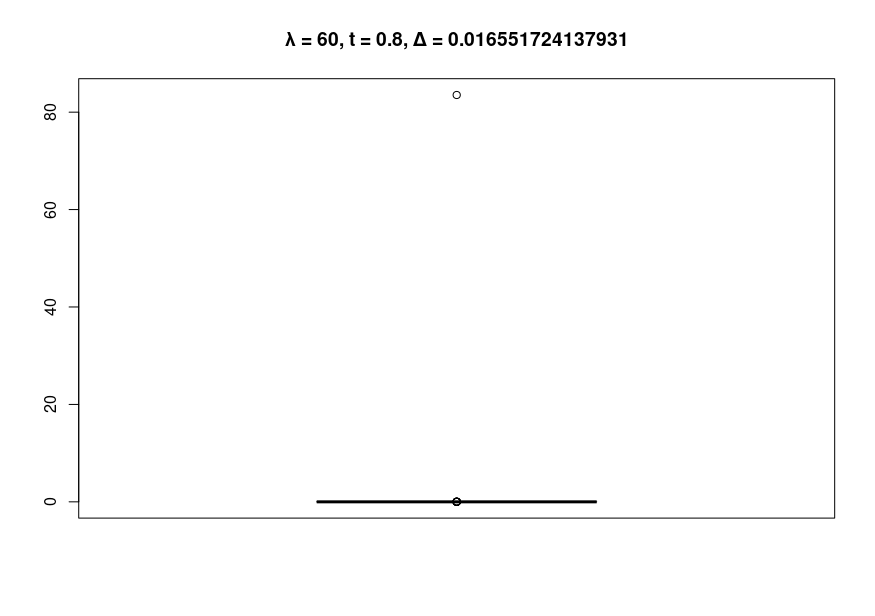
\includegraphics[width=0.47\textwidth]{Images/indiv_vs_glob/qq160.png}
		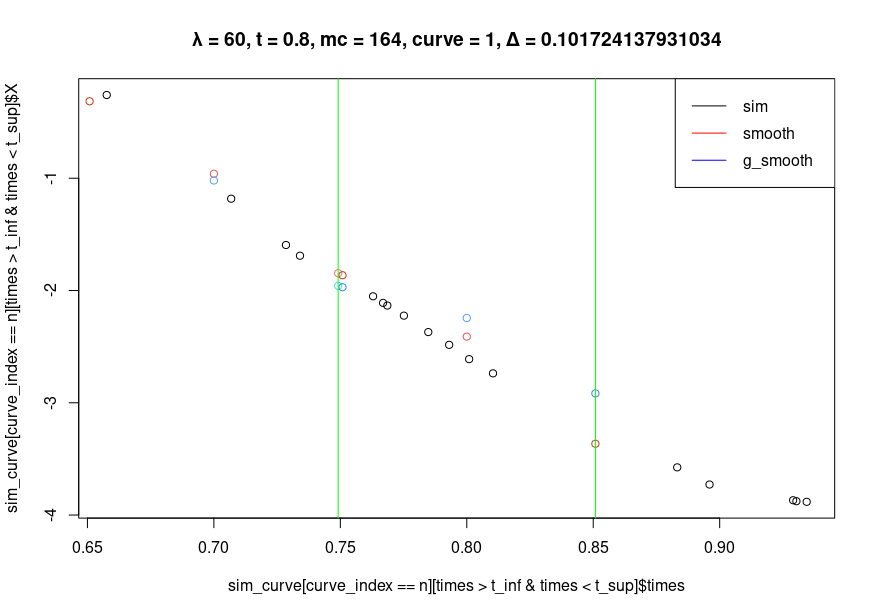
\includegraphics[width=0.47\textwidth]{Images/indiv_vs_glob/lbd60mc164c1.png}
	\end{minipage}

	\begin{minipage}{\linewidth}
		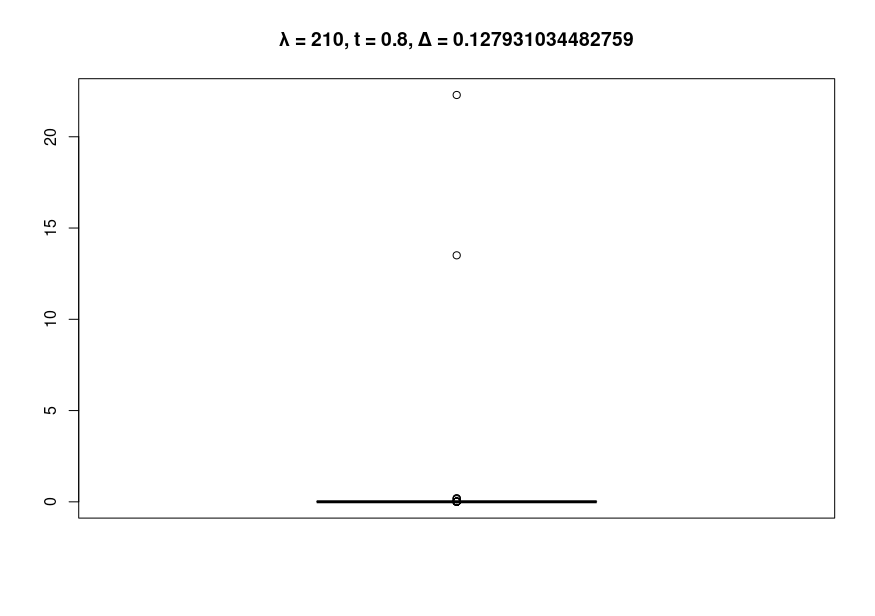
\includegraphics[width=0.47\textwidth]{Images/indiv_vs_glob/qq210.png}
		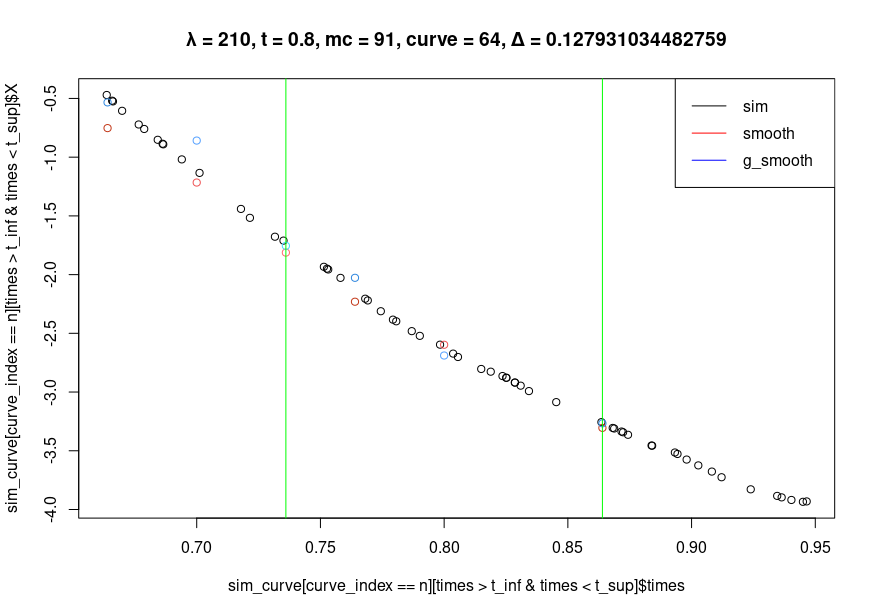
\includegraphics[width=0.47\textwidth]{Images/indiv_vs_glob/lbd210_mc91_c64.png}
	\end{minipage}
	\caption{Distribution des risques et aperçu d'une courbe pour un échantillon de monte carlo extrême sur le risque euclidien.}
	\label{fig:dist_R_eucl_curves}
\end{figure}

\begin{figure}[H]
	\centering
	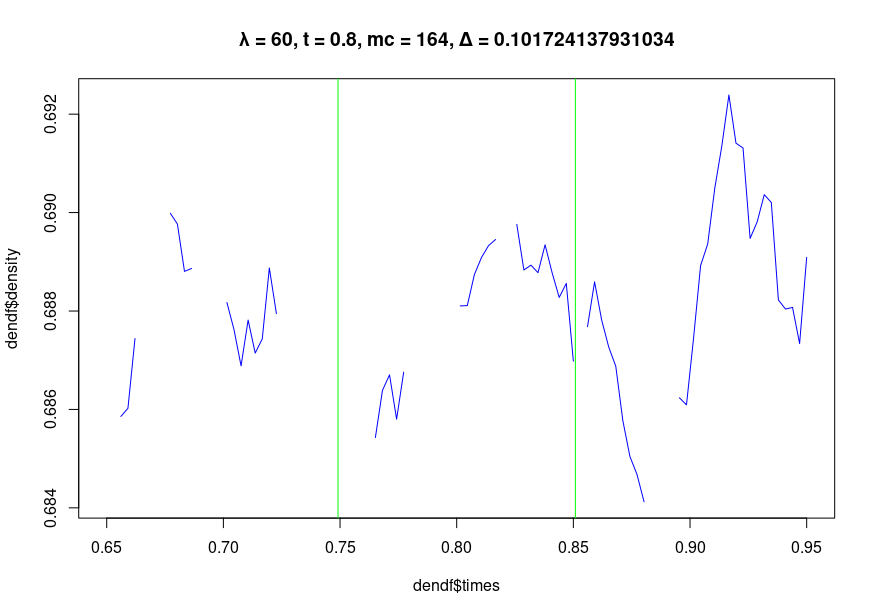
\includegraphics[width=0.7\textwidth]{Images/indiv_vs_glob/Tdensity_lbd60_mc164.png}
	\caption{Densité de points observés sur $[0.65, 0.95]$ pour $\lambda = 60$ sur un échantillon de monte carlo extrême, en un $\Delta$ problématique.}
	\label{fig:den_ex}
\end{figure}


\begin{figure}[H]
	\centering
	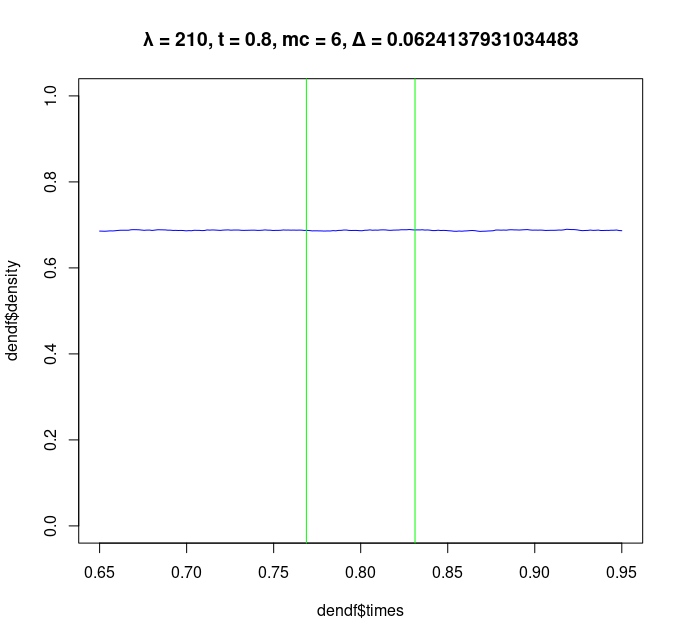
\includegraphics[width=0.4\textwidth]{Images/indiv_vs_glob/worst_210_67_mc6.png}
	\caption{Densité des points observés correspondant à la courbe présentée sur la figure \ref{fig:dist_R_eucl_curves}.}
	\label{fig:den_counterex}
\end{figure}

\begin{figure}[H]
	\centering

	\textbf{avec extrêmes : global}

	\includegraphics[width=0.9\textwidth]{Images/indiv_vs_glob_new/with_xtrm_glob/N200_λ210_t0.8_kernel.jpg}

	\textbf{avec extrêmes : individuel}

	\includegraphics[width=0.9\textwidth]{Images/indiv_vs_glob_new/with_xtrm/N200_λ210_t0.8_kernel.jpg}

	\textbf{sans extrêmes : individuel} (- top 2\%)

	\includegraphics[width=0.9\textwidth]{Images/indiv_vs_glob_new/no_xtrm/N200_λ210_t0.8_kernel.jpg}

	\textbf{sans extrêmes : global} (- top 2\%)

	\includegraphics[width=0.9\textwidth]{Images/indiv_vs_glob_new/no_xtrm_glob/N200_λ210_t0.8_kernel.jpg}
	\caption{Risque Euclidien pour $N=200$, $\lambda=210$ en un point régulier selon la méthode utilisée pour la fenêtre de lissage}
	\label{fig:compare_xtrm}
\end{figure}

\section{Etude de l'impact de la méthode de prélissage sur l'estimation de la régularité et le $\Delta$ optimal}
\label{annexe:prelissage_impact}
On peut aussi se poser la question suivante, traîtée ici en annexe pour ne pas flouter la mission principale de ce stage :

\question{
	$\circled 4$ : La méthode de pré-lissage utilisée possède-t-elle un impact important sur l'estimation de la régularité et donc sur la stratégie de sélection du $\Delta$ en pratique ?
}

\subsubsection{pré-lissage Spline}

Le lissage spline est certainement une des méthodes de lissage les plus répandues de par sa simplicité d'implémentation. De plus la détermination des hyper-paramètres de lissage via la méthode de GCV permet de déterminer une approximation de base optimale à un coût computationnel relativement faible. Un des plus grands avantages du lissage B-Spline est l'obtention d'une base de fonctions, qui permet à coût de stockage faible de pouvoir prédire des points non observés. Une fois la base déterminée, il ne reste plus qu'à prédire les points non observés en utilisant la base de fonctions et les coefficients de la décomposition de la courbe sur cette base.

\bigskip

On rappelle que l'utilisation de Splines comme méthode de lissage nécessite tout de même de faire des choix : elle est sensible aux nombre de noeuds et leur emplacement. Il est donc nécessaire de les déterminer par validation croisée. Une méthode fréquemment utilisée est d'utiliser un nombre de noeuds $\mathcal k$ égal au nombre d'observations, et de les placer aux points d'observations. Puis on utilise des splines pénalisées sur leur dérivée seconde ( $L = L_{quad} + \lambda \displaystyle\int_0^1 f''(u) du$ ) et on détermine le paramètre de pénalisation par validation croisée afin de s'affranchir du choix du nombre de noeuds et de leur emplacement. La validation croisée sur la pénalisation est supposée compenser ce choix. Il s'agit de la méthode qui a été utilisée dans le cadre de ce stage, car très populaire et simple à mettre en place.

Il est à noter qu'une autre méthode de lissage spline est de déterminer le nombre de noeuds $k$ par validation croisée, et de placer les points de façon uniforme sur les quantiles de la distribution des observations. Ce qui ne sera pas utilisé dans le cadre de ce stage.

\bigskip

En effectuant un pré-lissage de splines cubiques naturelles sur une courbe Höldérienne, on ne s'attend pas à obtenir de bonnes performances sur l'estimation de la régularité locale. En effet les courbes splines sont par construction de classe $\mathcal C^2$ (fonctions polynômiales $\mathcal C ^\infty$ avec des raccordements $\mathcal C^2$), et la courbe lissée écrasera complétement l'information de régularité. Même si il s'agit de ce que l'on souhaite obtenir et qu'on ne connait pas encore la régularité, il est raisonnable de penser qu'être précautionneux dans le choix de la technique de lissage de telle façon à être le plus proche de la régularité d'une fonction qui pourrait potentiellement ne même pas être dérivable est une bonne idée.



\subsubsection{pré-lissage à noyaux}

Considérer un lissage non paramétrique à noyaux est une alternative au lissage spline. L'espoir est la détermination lors du pré-lissage d'utiliser une fenêtre de lissage qui permette de mieux conserver l'information irrégulière que les splines via la détermination du $h^{*[\textsf{cv}]}_{\textsf{pre}}$ optimal par validation croisée.

\bigskip

Pour rappel, la fenêtre de lissage retenue est une fenêtre de lissage déterminée par validation croisée, qui est un estimateur de la fenêtre de lissage optimale pour le risque quadratique qui peut s'exprimer en fonction de la régularité locale si l'on suppose les hypothèses retenues sur le processus par MPV \cite{maissoro-SmoothnessFTSweakDep}. Même si le $h^*_{\mathcal R_{quadr}}$ est techniquement une fonction de $t \in \mathcal T$, l'estimateur que l'on considère lui sera sélectionné pour l'ensemble du support de la courbe $\mathcal T$. On peut espérer que si la courbe change de régularité sur son support mais que celui-ci ne varie pas trop, alors la fenêtre de lissage sélectionnée sera adaptée à la régularité locale de la courbe peu importe où l'on se trouve sur le support.


\subsubsection{Lisser en utilisant une base de fonction sans écraser l'information irrégulière ?}

Le lissage spline donne une fonction de classe $\mathcal C^2$, ce qui est un désavantage dans le cadre du prélissage qui sert à déterminer les paramètres de régularité de courbes issues d'un processus que l'on ne suppose pas plus régulier que continu. Toutefois, le fait d'utiliser une base de fonctions pour effectuer le lissage a de nombreux avantages par rapport au lissage à noyaux qui peuvent éventuellement s'avérer utiles dans certaines situations spécifiques pour la mise en production de modèles.

En effet, une fois que l'on a déterminé les composantes de la décomposition de notre signal sur la base de fonctions, on n'a plus besoin de se référer aux données pour prédire une valeur. Il s'agit d'une méthode très économe en mémoire, ce qui peut être très avantageux dans le cadre de la mise en production de modèles lorsqu'il y a de nombreuses courbes observées.




\subsection{Ondelettes}
\subsubsection{Une brève introduction aux ondelettes}

\input{content/chapter_2/02-regularite_locale/wavelet_intro.tex}

\subsubsection{Théorie de la base ondelettes}

\input{content/chapter_2/02-regularite_locale/wavelet_theorie.tex}


\subsubsection{Motivation dans le cadre de l'analyse de données fonctionnelles}

La capacité de capturer de façon efficiente les irrégularités de la fonction lissée est une motivation pour l'utilisation de la base d'ondelettes pour effectuer le pré-lissage de données, dont on espère qu'il n'écrase pas la majorité de l'information irrégulière de nos données. Si une des méthodes possibles, comme mentionnée précédemment, est d'utiliser un lissage non paramétrique à noyaux, les bases de fonctions ont de nombreux avantages. Un des avantage est le fait qu'une fois les projections sur la base déterminées, il n'y a plus besoin de se référer de nouveau aux données originales par la suite. Cela donne une représentation très parcimonieuse des données. Alors pour déterminer la valeur de $\widehat X(t)$ en un point $t$ non observé, il suffit d'évaluer l'expression $\sum_k \prodscal X {\psi_k} \psi_k(t)$.

\subsubsection{Effets du lissage à ondelettes sur la régularité locale}

\question{Peut on quantifier le biais introduit par le lissage en utilisant les ondelettes sur l'estimation de la régularité locale ?}

\editlater{regarder ce que ça donne, en utilisant les différents théorèmes et bornes disponibles sur les ondelettes pour un processus Holder LORSQUE J AI LE TEMPS - certainement en Septembre}


\chapter{Un peu d'Histoire}
\label{annexe:histoire}
\section{ Histoire des séries temporelles }
% \book{ \textbf{Un peu d'histoire sur les séries temporelles \ldots}        
\info{une grande partie des informations présentées dans cette section histoire provient de la référience ~\cite{time_series_brief_history} }


\smallskip

Parmi les étapes importantes du développement des séries temporelles, on peut noter l'article \emph{Time Series Analysis : Forecasting and Control} de Box et Jenkins (1970) qui introduit le modèle ARIMA et une approche aujourd'hui standarde d'évaluation du modèle à utiliser ainsi que son estimation. Ce développement est dû en grande partie à l'utilisation de telles données dans les secteurs économiques et des affaires afin de suivre l'évolution et la dynamique de différentes métriques

\smallskip

L'étude des séries temporelle a été divisée en l'étude du domaine fréquentiel, qui étudie le spectre des processus pour le décomposer en signaux principaux, et du domaine temporel, qui étudie les dépendances des indices temporels. L'utilisation de chacune des approches était sujet à débats mouvementés jusqu'aux alentours de l'an $2000$.

\smallskip

Le développement des capacités de calcul a été une révolution notamment pour l'identification des modèles (le critère AIC, l'estimation par vraissemblance dans les années $1980$, \ldots).
% modèles à espace d'états et le filtre de Kalman pour évaluer cette vraissemblance efficacement, MCMC, \ldots).

\smallskip

À partir des années $1980$, les modèles non linéaires émergent (ARCH par Engle, modèles à seuil \ldots) et trouvent application en économie notamment. Enfin l'étude multivariée (modèle VAR) fait surface dans les années 1980 par Christopher Sims~\cite[ \href{https://pubs.aeaweb.org/doi/pdf/10.1257/jep.15.4.101}{lien de l'article} ]{VAR_paper}

\smallskip

Une large partie de la théorie s'appuie notamment sur l'étude des racines de l'unité, en considérant un polynôme d'opérateur $P(B) = (I + \sum_k a_k B^k)$ à partir duquel les relations d'autocorrélations peuvent se ré-écrire.
% }
\pagebreak
\section{ Histoire des données fonctionnelles }
% \book{ \textbf{\ldots et un peu d'histoire sur les données fonctionnelles}
\info{Pour une description plus complète de l'histoire du développement de l'analyse fonctionnelle, on pourra se référer à \href{https://anson.ucdavis.edu/~mueller/fdarev1.pdf}{\textcolor{flatuicolors_blue_deep}{cet article de Wang, Chiou et Müller}}~\cite{wang2016functional}}


Bien que l'histoire du développement de l'Analyse de Données Fonctionnelles (FDA) puisse être retracée jusqu'aux travaux de Grenander et Karhunen~\cite{karhunen1946spektraltheorie} dans les années 1940 et 1950, où l'outil a été utilisé pour étudier les courbes de croissance en biométrie, ce sous-domaine de la statistique a été étudié de manière systématique à partir des années 1980.

\bigskip

En effet, c'est J.O. Ramsay qui a introduit l'appellation de "données fonctionnelles" en 1982~\cite{ramsay1982data} et qui contribuera en partie à sa popularisation. La thèse de Dauxois et Pousse en 1976 sur l'analyse factorielle dans le cadre des données fonctionnelles\cite{dauxois1976analyses} a ouvert la voie à l'analyse par composante principale fonctionnelle (FPCA), un outil clé pour l'étude des données fonctionnelles. La FPCA permet d'étudier des objets fonctionnels qui sont de dimension infinie, difficiles à manipuler et impossibles à observer empiriquement, en dimension finie et surtout sur $\R d$ que l'on connait bien.

\bigskip

Au cours des années 2000, de nombreux outils statistiques déjà développés pour des données à valeurs dans $\R d$ depuis un siècle, tels que la régression linéaire (éventuellement généralisée), les séries temporelles ou encore les modèles additifs, ont été adaptés aux données fonctionnelles.
Par exemple, les modèles de régression linéaire fonctionnelle ont été développés avec une réponse fonctionnelle~\cite{ramsay1991some} ou scalaire~\cite{cardot1999functional} en 1999.
Les modèles linéaires généralisés ont également été étudiés~\cite{james2002generalized,muller2005generalized}, avec l'estimation de la fonction de lien par méthode non paramétrique à direction révélatrice \emph{(Single Index Model)} récemment étudiée en 2011~\cite{chen2011single}.
Cette méthode avait déjà été utilisée en économétrie pour des données de $\R d$ depuis 1963~\cite{sharpe1963simplified}, et leur estimation directe a été étudiée une décennie auparavant par M.Hristache, Juditsky et Spokoiny~\cite{hristache2001direct}. De même, les modèles additifs ont été étendus aux données fonctionnelles en 1999 par Lin et Zhang~\cite{lin1999inference}.
Enfin, le livre de Bosq, \emph{\textcolor{flatuicolors_blue_devil}{Linear Processes in Function Spaces : Theory and Applications}}~\cite{bosq2000linear}, publié en 2000, a contribué au développement des séries temporelles pour les données fonctionnelles.

\bigskip

Depuis lors, des ressources telles que l'ouvrage de Kokoszka et Reimherr, \emph{\textcolor{flatuicolors_blue_devil}{Introduction to Functional Data Analysis (2017)}}~\cite{kokoszka2017introduction}, rendent la théorie et la mise en production des méthodes d'analyse et de prédiction de données fonctionnelles plus accessibles.
% }

\pagebreak
\section{Histoire du mouvement brownien et de ses applications}
\input{content/annexe/histoire_brownien.tex}


\pagebreak

% \chapter{Algorithmique}
% \label{annexe:algo}
% \section{Optimisation Algorithmique}

\subsection{Génération du bruit blanc}

pour générer un processus sous gaussien il nous faut inverser la matrice de covariance, qui dans notre a une dimension de :

\begin{equation*}
	\underbracket{\dim \vec\Delta}_{50} \times \underbracket{3}_{t_1 / t_2 / t_3} \times \underbracket{n_{points\_estim}}_{6} + \underbracket{n_{Grid\_\int}}_{100} + \underbracket{\lambda}_{\leq 480} \leq \underbracket{1000}_{fixe} + \underbracket{480}_{pts \, aleat}
\end{equation*}

on peut donc gagner du temps de calcul en inversant une unique fois la covariance restreinte aux points qui ne sont pas aléatoires et présents sur chaque courbe, ce qui peut faire la différence quand on a 400 courbes.

en posant :


\begin{align*}
	U & \isdef B \inverse D \\
	V & \isdef C \inverse A
\end{align*}


on obtient l'inversion de la matrice par blocs avec l'algorithme suivant :
\begin{equation*}
	\begin{bmatrix}
		A & B \\
		C & D
	\end{bmatrix}^{-1}
	=
	\begin{bmatrix}
		\inverse{(A - UC)} & 0                  \\
		0                  & \inverse{(D - VB)}
	\end{bmatrix}
	\begin{bmatrix}
		I   & - U \\
		- V & I
	\end{bmatrix}
\end{equation*}

dans notre cas
\begin{equation*}
	\Sigma = \begin{bmatrix}
		\Sigma_{[t \neg\textsf{ alea}]} & \Sigma_{[\textsf{alea} / \neg \textsf{ alea}]}
		\\ \Sigma^T_{[\textsf{alea} / \neg \textsf{ alea}]}
		                                & \Sigma_{[t \textsf{ alea}]}
	\end{bmatrix}
\end{equation*}

ce qui donnerait la formule d'inversion par bloc suivante :

$$
	\inverse \Sigma
	=
	\begin{bmatrix}
		\inverse{(\Sigma_{[t \neg\textsf{ alea}]} - UC)} & 0                                            \\
		0                                                & \inverse{(\Sigma_{[t \textsf{ alea}]} - VB)}
	\end{bmatrix}
	\begin{bmatrix}
		I   & - U \\
		- V & I
	\end{bmatrix}
$$

avec :

$U = \Sigma_{[\textsf{alea} / \neg \textsf{ alea}]} \inverse {\Sigma_{[t \textsf{ alea}]}} $

$V = \Sigma^T_{[\textsf{alea} / \neg \textsf{ alea}]} \inverse {\Sigma_{[t \neg\textsf{ alea}]}}$

\subsubsection{Intégrale}

\begin{equation*}
	X_{n+1}(t) = \int\limits_{[0,1]} \beta(u,t) \cdot \left[ X_{n-1}(u) - \mu(u)\right]du + \varepsilon_n
\end{equation*}

il est important lorsque l'on effectue autant de simulations d'avoir des calculs efficients pour limiter le temps de calcul.

Parmi les méthodes d'approximation d'intégrale classiques se trouvent les méthodes des rectangles, trapèze et de Newton-Cotes. On se basera sur la méthode de Newton Cotes d'ordre 0 aussi appelée des points médians pour l'avantage suivant : elle permet d'avoir à évaluer le Brownien fractionnaire en un seul point, ce qu'il signifie qu'on a besoin de générer qu'un seul point par sous-intervalle pour calculer l'intégrale, avec une approximation d'ordre 1 (ie, exacte pour un polynôme de degré $\leq 1$), plus précise que la méthode des rectangles à gauche et même des trapèzes.

\begin{equation*}
	\tilde E[g_{k}, g_{k+1}] = \frac{(g_{k+1}-g_k)^3}{12}f ^{''}(\eta_{k,k+1}) = \frac{(\frac{k+1} G - \frac k G )^3}{12}f ^{''}(\eta_{k,k+1}) = \frac{f ^{''}(\eta_{k,k+1})}{12G^3}
\end{equation*}


\begin{equation*}
	\tilde E = \frac 1 {12 G^3} \left[\sum_{k=0}^{G-1}f ^{''}(\eta_{k, k+1})\right] \leq \frac{\sup\limits_{[0,1]} f^{''} }{12 G^2}= \mathcal O\left( \frac 1 {G^2} \right)
\end{equation*}

Bien que nous ne manipulons pas des fonctions 2 fois dérivables, la borne d'approximation nous donne une idée de l'erreur qui sera commise en utilisant cette méthode.


\chapter{Algorithmes \& Implémentations}

\label{annexe:code}
\section{Algorithmes de simulation}

\begin{algorithm}[H]
	\caption{$\operatorname{Get\_single\_mc\_sim}$ : Génération de FAR pour chaque valeur sur la grille}\label{alg:gen_far_grid}
	\KwData{

	}
	\KwIn{
		$\vec t$ : endroits où évaluer la régularité

		Régularité de $X_n$ sur $[0,1]$ : $H : t \mapsto H_t$

		fonction moyenne : $\mu$
	}
	\KwOut{$L = \left\{ L[N, \lambda] : N \in \overrightarrow N, \lambda \in \lbdset   , n \in \nset \right\}$}
	\KwResult{$\simsetall$}


	\Comment*[l]{** ———— Paramètres utilisés ———— **}
	$G \gets 100$
	\Comment*[l]{Grille d'approximation de l'$\int$}\;


	$B \gets 100$
	\Comment*[l]{Burn-in de la relation FAR(1)}\;

	$\overrightarrow \Delta \gets \begin{bmatrix} 0.01 & \dots & 0.2\end{bmatrix}_{30}$
	\Comment*[l]{diamètre du voisinage $J_\Delta$}\;

	$\overrightarrow N \gets \begin{bmatrix} 100 & 200 & 300 & 400\end{bmatrix}_4$
	\Comment*[l]{nombre de courbes}\;

	$\mathbf \Lambda \gets \begin{bmatrix} 30 & 45 & \dots & 480 \end{bmatrix}$
	\Comment*[l]{nombre moyen de points observés sur une courbe}\;

	\Comment*[l]{** ———————————————————————————— **}

	$L = [ \quad ]$\;

	\For{$N \in \overrightarrow N$}{
	\Comment*[f]{$\overrightarrow N = [100, 200, 300, 400]$}

	\For{$\lambda \in \mathbf \Lambda$}{
		%{$\lambda\gets30$ \KwTo $480$ \KwBy $15$}{

		$\genxset \gets \operatorname{far\_sim}(N, \lambda, H, \mu, B, G, \vec t, \overrightarrow \Delta)$ \; \Comment*[f]{génération}

	}

	$L[N, \lambda] \gets \genxset$
	}

	\Return{$L$}
\end{algorithm}

\begin{algorithm}[H]
	\caption{Simulation de Monte Carlo}\label{alg:gen_far_mc}

	\For{ $\textsf{mc} \gets 1$ \KwTo $200$ }{
		$L_\textsf{mc} \gets \operatorname{Get\_single\_mc\_sim}(H, \mu)$
	}

	\Return{$\left\{ L_{\textsf{mc}} : \textsf{mc} \in \llbracket 1, 200 \rrbracket \right\}$}

\end{algorithm}

\begin{algorithm}
	\caption{$\operatorname{far\_sim}$ : Simulation d'un $\operatorname{FAR}(1)$}\label{alg:far_sim}
	\KwIn{
	$N \in \mathds N^*$ : nb $X_n$

	$\lambda \in \mathds N^*$ : nb moy pts observés

	$H : t \mapsto H_t$ : régularité

	$\mu : [0,1] \rightarrow \mathds R$ : moyenne

	$B \in \mathds N^*$ : Burn-in du FAR(1)

	$G \in \mathds N^*$ : grille méthode des rectangles

	$\overrightarrow \Delta$ : tous les diamètres testés

	$\vec t$ : endroits où évaluer la régularité
	}
	\BlankLine
	\KwResult{
		$\simset$

		avec $X_{n+1}(t) = \int \beta(u,t)X_n(t) + \eta_{n+1}$
	}

	\BlankLine
	\midrule
	\BlankLine
	$N_t \gets \operatorname{len}(\vec t)$\;
	$N_{calc} \gets N + B$
	\BlankLine

	\Comment*[l]{points de comparaison avec le lissage}
	$T(\Delta) = \begin{bmatrix} t_1[1] = \vec t[1] - \frac \Delta 2 & t_2[1] = \vec t[1] & t_3[1] = \vec t[1] + \frac \Delta 2 \\ \vdots & \vdots & \vdots \\  t_1[N_t] = \vec t[N_t] - \frac \Delta 2 & t_2[N_t] = \vec t[N_t] & t_3[N_t] = \vec t[N_t] + \frac \Delta 2 \end{bmatrix}$\;

	\BlankLine
	\Comment*[l]{Points observés}
	$T_{obs}\gets \mathcal U( [0,1] )^{\otimes \lambda}$\;

	\BlankLine
	\Comment*[l]{Grille de la méthode des rectangles médians}
	$\textsf{grid}_{\int} \gets \left( \frac{(k-1) + (k)}{2} \right)_{k \in \llbracket 1, G \rrbracket}$\;

	\BlankLine
	\Comment*[l]{Ensemble des points}
	$T \gets T_{obs}\bigcup T(\Delta) \bigcup \textsf{grid}_{\int}$\;

	$T \gets \operatorname{order}(T)$\;


	\BlankLine
	\BlankLine
	\Comment*[l]{Simulation de mouvement brownien multi fractionnaire de régularité $(H,L)$}
	$L = [ \quad ]$\;

	\For{$k \in \llbracket1 , N_{calc} \rrbracket$}{
		$\varepsilon_k \gets \operatorname{mfBm\_sim}(T, H, L)$\;

		$\mu_k \gets \mu(T)$\;

		$L[k] \gets \begin{bmatrix} T, \varepsilon_k, \mu_k \end{bmatrix}$\Comment*[f]{$\in \mathcal M_{\operatorname{len}T, 3}(\mathds R)$}\;
	}

	\BlankLine
	\BlankLine
	\Comment*[l]{Simulation de la relation FAR(1)}
	\Comment*[l]{$X_{n+1}(t) = \mu(t) + \displaystyle\int_0^1 \beta(u, t)X_n(u) du + \varepsilon_{n+1}$}
	\For{$k \in \llbracket1 , N_{calc} \rrbracket$}{
		$K_\beta = \begin{bmatrix} \ddots & \vdots & \rddots \\ \dots & \beta(s,t) & \dots \\ \rddots & \vdots & \ddots  \end{bmatrix}$\;
		$I(\beta, \mathds X_{k-1}) = \frac 1 G  K_\beta \mathds X_{k-1}$\;
		$\mathds X_k \gets \mu_k + I(\beta, \mathds X_{k-1}) + \varepsilon_k$\;
	}

	\Return{ $(\mathds X_n)_{n \in \llbracket B+1, N_{calc} \rrbracket}$ }
\end{algorithm}

\pagebreak

\section{Implémentation R}
\label{annexe:code-R}
\section{packages utilisés}

\begin{minted}[linenos=true, mathescape=true, frame=single, breaklines]{R}
    # ——— install ——— #
    install.packages(c("data.table","wavethresh","fda", "fda.usc"))
    # ——— general packages ——— #
    library(data.table)
    # ——— FDA packages ——— #
    library(fda)
    library(fda.usc)
    # ——— Wavelet packages ——— #
    library(wavethresh)
\end{minted}

\section{Simulation des FAR}


\section{Lissage des courbes}


\section{Détermination de la régularité locale}


\section{Détermination des risques}


\section{Lissage adaptatif}

Dans la section \ref{sec:lissage_adapt}, nous avons mentionné qu'il était judicieux de lisser les courbes de façon adaptative à la quantité que l'on souhaite estimer. Si l'on a mentionné le risque à minimiser pour chaque quantité que l'on souhaite estimer, aucun détail n'a été fourni car il alourdit considérablement la trame de l'objectif du stage sans apporter des informations cruciales.

\bigskip

Cependant pour l'implémentation d'un tel lissage adaptatif, il fallait évidemment se référer au détail de l'expression pour pouvoir évaluer ce risque et déterminer la meilleure fenêtre.

\bigskip

\begin{equation*}
	R_\mu( \, t \, , h \, ) =
	\underbracket{L_t^2 h ^{2H_t} \mathds B( \, t, h, 2H_t \,) }_{\textsf{contrôle du biais}}
	+ \underbracket{\sigma^2 \mathds V_\mu( \, t, h \, ) }_{\textsf{contrôle de la variance}}
	+ \underbracket{\frac{\mathds D_\mu( \, t \, )}{P_N(t, h)}}_{\textsf{contrôle de la dépendance}}
\end{equation*}

Développons maintenant les différentes quantités présentes dans l'expression :

\begin{equation*}
	{\mathds D_\mu( \, t \, )} \isdef
\end{equation*}
\begin{equation*}
	\mathds V_\mu( \, t, h \, ) \isdef
\end{equation*}
\begin{equation*}
	\mathds B( \, t, h, 2H_t \,) \isdef
\end{equation*}
\begin{equation*}
	P_N(t, h) \isdef
\end{equation*}




\chapter{
  Analyse du comportement du $\Delta$ : autres métriques non retenues
 }

\section{Qualité de l'estimation des incréments quadratiques moyens}

\newcommand{\thetaA}{\Theta_{1 \rightarrow \overset{3}{\underset {2}{}}}}
\newcommand{\cindexA}{_{1 \rightarrow \overset{3}{\underset {2}{}}}}
\newcommand{\thetaB}{\Theta_{\overset 1{\underset{2}{ }} \rightarrow3}}
\newcommand{\cindexB}{_{\overset 1{\underset{2}{ }} \rightarrow3}}
\newcommand{\thetaC}{\Theta_{1 \rightarrow 2 \rightarrow 3}}
\newcommand{\cindexC}{_{1 \rightarrow 2 \rightarrow 3}}
\newcommand{\notequiv}{\overset {\textsf{\faTimes}} \iff}
\newcommand{\yesequiv}{\overset {\textsf{\faCheck}} \iff}

Il y a différentes manières de définir les paramètres de régularité $\hat H_t$ et $\hat L_t$. En effet il est possible de définir $\hat H_t$ en utilisant $\hat \theta (t_1, t_2)$ mais aussi en utilisant $\hat \theta (t_2, t_3)$ ($\theta(t_1, t_3)$ est forcément utilisé\footnote{$\hat H_t$ ne serait même pas bien défini pour le couple $\theta(t_1, t_2)$, $\theta(t_2, t_3)$}). De même pour $\hat L_t$. On peut donc se demander quels sont les meilleurs $\theta(u,v)$ avec $u,v \in \{t_1, t_2, t_3\}$ à utiliser pour obtenir la meilleure estimation de $H_t$ et $L_t$ ainsi que leur $\Delta$ optimal associé pour l'estimation de ces paramètres.

\bigskip

Le problème est que le proxy $\theta$ est défini comme une espérance, et donc n'est pas observable. On ne peut donc pas directement comparer $\hat \theta(u,v) = \sum_i|\widehat X_i(u) - \widehat X_i(v)|^2$ et $\theta(u,v) = \esperanceloi X { |X(u) - X(v)|^2 }$, à moins d'avoir fait le calcul de l'expression explicite en connaissant la loi du processus initial.

\bigskip

On peut cependant comparer $\hat \theta(u,v)$ et $\widetilde \theta(u,v) = \frac 1 N \sum_i |X_i(u) - X_i(v)|^2$ qui est un estimateur de $\theta(u,v)$, et que l'on obtient aisément avec la simulation. On peut ainsi déterminer pour quelle valeur de $\Delta$ et quel couple $(u,v)$ on dispose de la meilleur estimation du $\tilde \theta$, qui est entre-autre le meilleur estimateur que l'on pourrait espérer de $\theta$. Le meilleur couple (au sens donné dans cette section) est pris comme étant les deux $\hat \theta(u,v)$ réalisant les risques minimaux par rapport au $\tilde \theta$ sur les 3 couples $(u,v)$ possibles.

\begin{table}[H]
	\centering
	\begin{tabular}{l|ll|}
		\cline{2-3}
		                                     & $\lambda < 120$                                                                                            & $\lambda \geq 120$                                                                 \\ \hline
		\multicolumn{1}{|l|}{$H_t < 0.6$}    & \multicolumn{1}{l|}{\begin{tabular}[c]{@{}l@{}}$\thetaC$\\ \\ \\ $\Delta^- \rightarrow 0.01$\end{tabular}} & \begin{tabular}[c]{@{}l@{}}$\thetaA$\\ \\ $\Delta^+ \rightarrow 0.2$\end{tabular}  \\ \cline{2-3}
		\multicolumn{1}{|l|}{$H_t \geq 0.6$} & \multicolumn{1}{l|}{\begin{tabular}[c]{@{}l@{}}$\thetaA$\\ \\ $\Delta^- \rightarrow 0.2$\end{tabular}}     & \begin{tabular}[c]{@{}l@{}}$\thetaC$\\ \\ $\Delta^+ \rightarrow 0.01$\end{tabular} \\ \hline
	\end{tabular}
	\caption{Tableau récapitulatif des $\Theta$ optimaux : Risque individuel sur $\tilde \theta(u,v)$}
	\label{tab:recap_theta_single}
\end{table}


\section{Qualité de l'estimation de la régularité locale}

Les simulations de Monte Carlo permettent d'avoir accès directement à la véritable régularité de la courbe en chaque point. Nous allons dans l'étude du comportement du $\Delta$ essayer de tirer profit de cet avantage que ne possède pas le praticien qui utilise des données réelles.


\begin{table}[H]
    \centering
    \begin{tabular}{l|ll|}
        \cline{2-3}
                                              & $\lambda < 120$                                                                                                                                                                                                    & $\lambda \geq 120$                                                                                                                                        \\ \hline
        \multicolumn{1}{|l|}{$H_t \leq 0.65$} & \multicolumn{1}{l|}{\begin{tabular}[c]{@{}l@{}}$\yesequiv \mathcal R$\\ $\yesequiv \Delta^*$\\ $\Delta^- \downarrow 0.01$\end{tabular}}                                                                            & \begin{tabular}[c]{@{}l@{}}$\simeq \yesequiv \mathcal R$\\ $\notequiv \Delta^*$\\ $\Delta^+ \rightarrow [\leq 0.6] 0.1/0.2 [\geq 0.6]$\end{tabular}        \\ \cline{2-3}
        \multicolumn{1}{|l|}{$H_t > 0.65$}    & \multicolumn{1}{l|}{\begin{tabular}[c]{@{}l@{}}$\yesequiv \mathcal R$\\ $\notequiv \Delta^*$\\ \faExclamationTriangle $H=0.7 : \Delta^- = 0.02$\\ \faExclamationTriangle $H = 0.73 : \Delta^- = 0.2$\end{tabular}} & \begin{tabular}[c]{@{}l@{}}$\thetaA$\\ \faExclamationTriangle $H=0.7 : \Delta^+ = 0.02$\\ \faExclamationTriangle $H = 0.73 : \Delta^+ = 0.2$\end{tabular} \\ \hline
    \end{tabular}
    \caption{Tableau récapitulatif des $\Delta$ optimaux : Risque sur $H_t$}
    \label{tab:recap_delta_H}
\end{table}



%%%%%%%%%%%%%%%%%%%%%%%%% FIN CHAPITRES %%%%%%%%%%%%%%%%%%%%%%%%%%%%%%%%

\typeout{}
\bibliography{bibliography/main}

\end{document}
